%% KUEzh Matura thesis template
% Template version used: v3
%
% Largely adapted from Adrian Nievergelt's template for the ADPS
% (lecture notes) project which was adapted by Karel Kubicek from whom I adpated it. This template is under the CC0 license.

% Electronic version that does not waste space
\documentclass[11pt,a4paper,openany,oneside]{memoir}

% Printable version that does waste space (but people like it), uncomment for printing. Only use for printing
%\documentclass[11pt,a4paper,final]{memoir}
\usepackage{glossaries}
\usepackage{graphicx}
\usepackage{subcaption}
\usepackage{tikz}
\usetikzlibrary{shapes.geometric, arrows}
\usepackage{ wasysym }
%% Packages
%% ========

%% LaTeX Font encoding -- DO NOT CHANGE
\usepackage[OT1]{fontenc}

% German (Don't change)
\usepackage[ngerman]{babel}

% uft8 is the standard for web. Use this (alternative utf8x if you run into issues)
\usepackage[utf8]{inputenc}


%% excellent Palatino font.  Do not change this.
\usepackage[sc]{mathpazo}

%% The AMS-LaTeX extensions for mathematical typesetting.  Do not
%% remove.
\usepackage{amsmath,amssymb,amsfonts,mathrsfs}

% Do not remove (for theorems like proofs)
\usepackage[amsmath,thmmarks]{ntheorem}

%% LaTeX' own graphics handling
\usepackage{graphicx}

%% We unfortunately need this for the Rules chapter.  Remove it
%% afterwards; or at least NEVER use its underlining features.
\usepackage{soul}

%% This allows you to add .pdf files. This is used for the logo
\usepackage{pdfpages}

%% Some more packages that you may want to use.  Have a look at the
%% file, and consult the package docs for each.
%% See the TeXed file for more explanations

%% [OPT] Multi-rowed cells in tabulars
%\usepackage{multirow}

%% Make document internal hyperlinks wherever possible. (TOC, references)
%% This MUST be loaded before cleveref
\usepackage[linkcolor=black,colorlinks=true,citecolor=black,filecolor=black]{hyperref}
\usepackage[acronym]{glossaries}
%% [REC] Intelligent cross reference package. This allows for nice
%% combined references that include the reference and a hint to where
%% to look for it.
%% Template v2: cleveref already recognizes what is being referenced - one does not need to write Fig./Sec.
% \usepackage{varioref}. Capitalization is prefered in CS
\usepackage[capitalise]{cleveref}
\usepackage{algpseudocode}
%% [OPT] Easily changeable quotes with \enquote{Text}
\usepackage[german=swiss]{csquotes}
\usepackage{algorithm}
%% Template v2: this prevents warning "Package fmtcount Warning: \ordinal already defined use \FCordinal instead. on input line". See https://tex.stackexchange.com/questions/162353/memoir-class-conflict-with-datetime#comment371926_162358
\let\ordinal\relax
%% [REC] Format dates and time depending on locale
\usepackage{datetime}

%% [OPT] Provides a \cancel{} command to stroke through mathematics.
%\usepackage{cancel}

%% [NEED] This allows for additional typesetting tools in mathmode.
%% See its excellent documentation.
\usepackage{mathtools}

%% [ADV] Conditional commands
%\usepackage{ifthen}

%% [OPT] Manual large braces or other delimiters.
%\usepackage{bigdelim, bigstrut}

%% [REC] Alternate vector arrows. Use the command \vv{} to get scaled
%% vector arrows.
\usepackage[h]{esvect}

%% [NEED] Some extensions to tabulars and array environments.
\usepackage{array}

%% [OPT] Postscript support via pstricks graphics package. Very
%% diverse applications.
%\usepackage{pstricks,pst-all}

%% [?] This seems to allow us to define some additional counters.
%\usepackage{etex}

%% [ADV] XY-Pic to typeset some matrix-style graphics
%\usepackage[all]{xy}

%% [OPT] This is needed to generate an index at the end of the
%% document.
%\usepackage{makeidx}

%% [OPT] Fancy package for source code listings.  The template text
%% needs it for some LaTeX snippets; remove/adapt the \lstset when you
%% remove the template content.
\usepackage{listings}
\lstset{language=TeX,basicstyle={\normalfont\ttfamily}}

% Template v2 fixes: this is an old package, microtype is superior + fixes an error
%% [REC] Fancy character protrusion.  Must be loaded after all fonts.
\usepackage[activate]{microtype}
% \usepackage[activate]{pdfcprot}  % causes the compilation error

%% [REC] Nicer tables.  Read the excellent documentation.
\usepackage{booktabs}


%% Our layout configuration.  DO NOT CHANGE.
%% Memoir layout setup

%% NOTE: You are strongly advised not to change any of them unless you
%% know what you are doing.  These settings strongly interact in the
%% final look of the document.

% Dependencies
\usepackage{kue-template/KUElogo}

% Turn extra space before chapter headings off.
\setlength{\beforechapskip}{0pt}

\nonzeroparskip
\parindent=0pt
\defaultlists

% Chapter style redefinition
\makeatletter

\if@twoside
  \pagestyle{Ruled}
  \copypagestyle{chapter}{Ruled}
\else
  \pagestyle{ruled}
  \copypagestyle{chapter}{ruled}
\fi
\makeoddhead{chapter}{}{}{}
\makeevenhead{chapter}{}{}{}
\makeheadrule{chapter}{\textwidth}{0pt}
\copypagestyle{abstract}{empty}

\makechapterstyle{bianchimod}{%
  \chapterstyle{default}
  \renewcommand*{\chapnamefont}{\normalfont\Large\sffamily}
  \renewcommand*{\chapnumfont}{\normalfont\Large\sffamily}
  \renewcommand*{\printchaptername}{%
    \chapnamefont\centering\@chapapp}
  \renewcommand*{\printchapternum}{\chapnumfont {\thechapter}}
  \renewcommand*{\chaptitlefont}{\normalfont\huge\sffamily}
  \renewcommand*{\printchaptertitle}[1]{%
    \hrule\vskip\onelineskip \centering \chaptitlefont\textbf{\vphantom{gyM}##1}\par}
  \renewcommand*{\afterchaptertitle}{\vskip\onelineskip \hrule\vskip
    \afterchapskip}
  \renewcommand*{\printchapternonum}{%
    \vphantom{\chapnumfont {9}}\afterchapternum}}

% Use the newly defined style
\chapterstyle{bianchimod}

\setsecheadstyle{\Large\bfseries\sffamily}
\setsubsecheadstyle{\large\bfseries\sffamily}
\setsubsubsecheadstyle{\bfseries\sffamily}
\setparaheadstyle{\normalsize\bfseries\sffamily}
\setsubparaheadstyle{\normalsize\itshape\sffamily}
\setsubparaindent{0pt}

% Set captions to a more separated style for clearness
\captionnamefont{\sffamily\bfseries\footnotesize}
\captiontitlefont{\sffamily\footnotesize}
\setlength{\intextsep}{16pt}
\setlength{\belowcaptionskip}{1pt}

% Set section and TOC numbering depth to subsection
\setsecnumdepth{subsection}
\settocdepth{subsection}

%% Titlepage adjustments
\pretitle{\vspace{0pt plus 0.7fill}\begin{center}\HUGE\sffamily\bfseries}
\posttitle{\end{center}\par}
\preauthor{\par\begin{center}\let\and\\\Large\sffamily}
\postauthor{\end{center}}
\predate{\par\begin{center}\Large\sffamily}
\postdate{\end{center}}

\def\@advisors{}
\newcommand{\advisors}[1]{\def\@advisors{#1}}
\def\@department{}
\newcommand{\department}[1]{\def\@department{#1}}
\def\@thesistype{}
\newcommand{\thesistype}[1]{\def\@thesistype{#1}}

\renewcommand{\maketitlehooka}{
\includegraphics[scale=0.4]{kue-template/kuezh.pdf}}

\renewcommand{\maketitlehookb}{\vspace{1in}%
  \par\begin{center}\Large\sffamily\@thesistype\end{center}}

\renewcommand{\maketitlehookd}{%
  \vfill\par
  \begin{flushright}
    \sffamily
    \@advisors\par
    \@department, Kantonsschule Uetikon am See
  \end{flushright}
}

\checkandfixthelayout

\setlength{\droptitle}{-48pt}

\makeatother

% This defines how theorems should look. Best leave as is.
\theoremstyle{plain}
\setlength\theorempostskipamount{0pt}

%%% Local Variables:
%%% mode: latex
%%% TeX-master: "thesis"
%%% End:


%% Theorem environments.  You will have to adapt this for a German
%% thesis.
%% Theorem-like environments

%% This can be changed according to language. You can comment out the ones you
%% don't need.

\numberwithin{equation}{chapter}

%% German theorems
\newtheorem{satz}{Satz}[chapter]
\newtheorem{beispiel}[satz]{Beispiel}
\newtheorem{bemerkung}[satz]{Bemerkung}
\newtheorem{korrolar}[satz]{Korrolar}
\newtheorem{definition}[satz]{Definition}
\newtheorem{lemma}[satz]{Lemma}
\newtheorem{proposition}[satz]{Proposition}



%% English variants
%\newtheorem{theorem}{Theorem}[chapter]
%\newtheorem{example}[theorem]{Example}
%\newtheorem{remark}[theorem]{Remark}
%\newtheorem{corollary}[theorem]{Corollary}
%\newtheorem{definition}[theorem]{Definition}
%\newtheorem{lemma}[theorem]{Lemma}
%\newtheorem{proposition}[theorem]{Proposition}

%% Proof environment with a small square as a "qed" symbol
\theoremstyle{nonumberplain}
\theorembodyfont{\normalfont}
\theoremsymbol{\ensuremath{\square}}
\newtheorem{proof}{Proof}
%\newtheorem{beweis}{Beweis}


%% Helpful macros.
%% Custom commands
%% ===============

%% Special characters for number sets, e.g. real or complex numbers.
\newcommand{\C}{\mathbb{C}}
\newcommand{\K}{\mathbb{K}}
\newcommand{\N}{\mathbb{N}}
\newcommand{\Q}{\mathbb{Q}}
\newcommand{\R}{\mathbb{R}}
\newcommand{\Z}{\mathbb{Z}}
\newcommand{\X}{\mathbb{X}}
\newcommand{\ac}[1]{\acrshort{#1}}


%% Fixed/scaling delimiter examples (see mathtools documentation)
\DeclarePairedDelimiter\abs{\lvert}{\rvert}
\DeclarePairedDelimiter\norm{\lVert}{\rVert}

%% Use the alternative epsilon per default and define the old one as \oldepsilon
\let\oldepsilon\epsilon
\renewcommand{\epsilon}{\ensuremath\varepsilon}

%% Also set the alternate phi as default.
\let\oldphi\phi
\renewcommand{\phi}{\ensuremath{\varphi}}
\renewcommand{\dq}{\textquotedbl}

\makeglossaries
% Template v2: BibLaTeX with Biber backend are in my opinion best maintainable citation configurations. IEEE style is common in CS.
% Bibliography
\usepackage[
bibstyle=ieee,
citestyle=ieee,
isbn=true,
doi=true,
sorting=none,
url=true,
 defernumbers=true,
bibencoding=utf8,
backend=biber
]{biblatex} %Imports BibLaTeX package
\addbibresource{refs.bib}
\addbibresource{zotero.bib} %Import the bibliography file

%% ====================

\title{Entwurf, Konstruktion und Bau eines autonomen Segelboots}
\author{Georg Alejandro Niggli}
\thesistype{Schweizer Jugend Forscht}
\advisors{Betreung: Dr. Carola Ebenhoch}
\department{Fachschaft Physik}
\date{30.3.2025}
\begin{document}

\frontmatter

%% Title page is autogenerated from document information above.  DO
%% NOT CHANGE.
\begin{titlingpage}
  \calccentering{\unitlength}
  \begin{adjustwidth*}{\unitlength-24pt}{-\unitlength-24pt}
    \maketitle
  \end{adjustwidth*}
\end{titlingpage}

%% The abstract of your thesis.  Edit the file as needed.
\begin{abstract}
Autonome Fahrzeuge gewinnen zunehmend an Bedeutung. Auch auf Gewässern bieten sie vielfältige Einsatzmöglichkeiten, darunter beispielsweise die Überwachung der Wasserqualitat an verschiedenen Standorten. Segelboote erweisen sich aufgrund ihrer Emissionsfreiheit und ihres geringen Energiebedarfs als besonders geeignet für solche Einsatzzwecke. In dieser Arbeit wird der Entwurf, die Konstruktion und der Bau eines autonomen Segelboots untersucht, und der Bau eines kostengünstigen Prototypen beschrieben.

\end{abstract}


%% TOC with the proper setup, do not change.
\cleartorecto
\tableofcontents
\mainmatter

%% Your real content!
%\setkeys{Gin}{draft} %% Toggle images with adding a % in the front of this line for faster compile time

\chapter{Einleitung }
\label{chap:einleitung}
Segelboote waren vor der Erfindung motorisierter Boote und Schiffe der Schlu¨ssel zur Globalisierung. Dank der Kraft des Windes konnten Menschen damals riesige Distanzen überwinden und Güter selbst über Ozeane transportieren. Seit der Erfindung der der Dampfmaschine und der damit ausgelösten industriellen Revolution dienen sie jedoch fast nur noch als Vergnu¨gungs- oder Sportgeräte. Mit der immer verfu¨ gbar werde- derderen Technologie des autonomen Fahren können Segelboote einen erneuten Aufschwung erleben.


\section{Heutige Verbreitung von Autonomen Segelbooten}
Während Berichte über Entwicklungen und Fortschritte autonomer Strassenfahrzeuge fast täglich in der Presse erscheinen und sich die bedeutendsten und kapitalkräftigsten Unternehmen der Fahrzeugindustrie und Informatik in einem harten Wettbewerb um die Führerschaft bei deren Entwicklung befinden (siehe https://de.wikipedia.org/wiki/Autonomes\_Fahren), verläuft die Entwicklung von autonome Segelboten ………Nische 

\section{Was sind autonome Segelboote}
\subsection{Segelboot}
Ein Schiff ist in Wasserfahrzeug oder ein anderer zur Fortbewegung auf oder unter der Wasseroberfläche bestimmter Schwimmkörper, oder ein schwimmendes Gerät (Artikel 2 Abs. 1 lit. a Ziffer 1 der Verordnung über die Schifffahrt auf schweizerischen Gewässern (Binnenschifffahrtsverordnung, BSV) vom 8. November 1978. Ein Boot ist damit ein Schiff, wobei der Begriff Schiff als Überbegriff für Wasserfahrzeuge gilt und der Begriff Boot regelmässig zur Bezeichnung kleineren Wasserfahzeugen wie Ruderbooten, Sportboote, Paddelbooten etc. dient, die in der Regel nicht eingedeckt sind (https://de.wikipedia.org/wiki/Boot). 

Ein Segelschiff ist ein Schiff, das für die Fortbewegung mit Segeln versehen ist; ein Segelschiff, das mit oder ohne gesetzte Segel unter Motor fährt, gilt im Sinne der Verkehrsvorschriften als Schiff mit Maschinenantrieb (Artikel 2 Abs. 1 lit. a Ziffer 9 der Verordnung über die Schifffahrt auf schweizerischen Gewässern (Binnenschifffahrtsverordnung, BSV) vom 8. November 1978. Ein Schiff ist folglich nur dann ein Segelschiff, wenn es 

 (a) für die Fortbewegung mit Segeln versehen ist, und 

 (b) über keinen Motor für die Fortbewegung verfügt oder einen vorhandenen Motor nicht dafür einsetzt. 

Der Einsatz von Motoren für andere Zwecke als der Fortbewegung, zum Beispiel für das Setzen von Segeln oder das Bewegen des Ruders, ändert aber nichts an der Klassierung eines Wasserfahrzeuges als Segelschiff. 

\subsection{Autonomie}
Unbemannt und ohne eigene Mannschaft und nicht ferngesteuert (Gegensatz zum Roboter)

Autonom ist ein Segelboot, das selbst, also autonom und ohne eigene Mannschaft operieren kann. Es benötigt einzig die Vorgabe ein es Ziels und findet danach selbständig den Weg an dieses vorgegebene oder allenfalls mehrere vorgegebene Ziele. Autonome Boote unterscheiden sich damit von Roboterschiffen oder Drohenschiffen, die ferngesteuert operiert werden. 

Ein autonomes Segelboot muss nach einer einmaligen Vorgabe eines Zielpunktes, seine Position auf dem Gewässer selbständig ermitteln, das Ziel unter Nutzung der Windkraft selbständig ansteuern, den gewählten Kurs den herrschenden und sich ändernden Umweltbedingungen wie Wind oder Strömung selbständig so anpassen, dass es das Ziel ohne Eingriffe einer Mannschaft unter Nutzung der Windenergie planmässig und nicht nur zufällig erreicht.


\section{Weshalb Autonome Segelboote an Bedeutung gewinnen könnten}

\section{Mögliche Konkrete Einsatzbereiche}
\subsection{Schadstoffbelastung am Chemieareal Uetikon am See}
Das Chemieareal ist ein Bereich direkt am Zürichsee, welches durch jahrelange Umweltverschmutzung und Belastung von Schwermetallen geprägt wurde. Beim Umbau des Areals in eine Schule und Wohnungskomplexe müssen die toxischen Überresten der Industrie entfernt werden. Dieser Entfernungsprozess gilt als sicher und viele Massnahmen um eine Vermeindung von Freisetzung von toxischem Material werden getroffen. Jedoch werden Gewässerproben um die Einhaltung der Wasserqualität nur sporadisch gemacht. Es Gefährt, welches während den Arbeiten einen grossen Bereich sehr kostengünstig überwachen könnte, wäre hier von Vorteil. Da an einem Segelboot Sensoren jegliche Art angebracht werden können, kann neben Verunreinigungen auch durch SONAR der Seeboden kartografiert werden oder das verhalten von Fischpopulationen überwacht werden. All dies sind äusserst wertvolle Daten, welche bis jetzt nur schwer regelmässig zu beschaffen waren. Sobald die Arbeiten abschlossen sind, könnte der Bereich für einen längeren Zeitraum überwach. um zu überprüfen ob die gemachte Arbeit auch den Annahmen standhält.

\subsection{Grosse Seen}
// Grosse seen komplett monitoren und über das ganze Jahr veränderungen am Seeboden feststellen

\section{Zielsetzung}
Das Ziel dieser Arbeit ist ein autonomes Segelboot von Grund auf neu zu entwickeln. 

Dazu soll mittels eines \href{https://www.overleaf.com/project/64c425dc65e5d82bb7de603c\#_bookmark0}{CAD}-Programmes (CAD = Computer Aided Design) computergestützt ein Segelboot entworfen werden, um anschliessend nach den mit dem CAD-Programm erstellten Plänen gebaut zu werden. Das Segelboot soll mit allen zur autonomen Navigation und Steuerung erforderlichen Geräten, Rechnern und Sensoren sowie der zu deren Betrieb erforderlichen autonomen Energieversorgung ausgerüstet werden. Schliesslich soll das Segelboot mit Programmen ausgestattet werden, die es ihm erlauben, bei allen möglichen Windrichtungen den vordefinierten Zielpunkt anzusteuern und selbst bei einer Veränderung der Windrichtung selbständig zu erreichen.

Kostengünstig mit Materialen aus Baumarkt und Elektronikversand und Heimwerkerausrüstung


\section{Aufbau der Arbeit}
In einem ersten Teil wird die 

 Konzeption, der Entwurf, die Konstruktion und der Bau des Bootskörpers sowie des Segels beschrieben. In einem zweiten Teil wird die

  Im Abschnitt über die technische/elektrische Ausrüstung des Bootes, insbesondere der verwendet Rechner und die Überlegungen zu dessen Wahl, die eingesetzten Sensoren, die Stromversorgungslösung und die Lengsteuerung diskutiert.

 In einem nächsten Teil werden nach einer knappen Einführung in die Grundlagen der Physik des Segelns, die Überlegungen zur Architektur der Naviationssoftware, die Navigation und die Wegfindung diskutiert

 In einem ….. Teil wird der Bau der Bestandteile des Bootskörpers und des Segels und anschliessende Zusammenbau und die Montage beschrieben 

  
\input{kapitel/literaturübersicht}

\chapter{Konzeptentwicklung }
\label{chap:konzeptentwicklung}
\section{Zielsetzung}
Das Ziel dieser Arbeit ist es, ein autonomes Segelboot zu entwerfen, zu konstruieren und zu bauen. Dabei soll günstiges und einfach zu verarbeitendes Konstruktonsmaterial verwendet werden, das in Baumärkten erworben werden kann, mit Werkzeugen gearbeitet werden, die in einer gut bestückten Handwerkerwerkstatt vorhanden sind, die Navigation und Steuerung selbst entworfen werden und die dafür notwendigen Programme selbst entwickelt werden. 

%?????? Dazu soll mittels eines CAD-Programmes (CAD = Computer Aided Design) computergestützt ein Segelboot entworfen werden, um anschliessend nach den mit dem CAD-Programm erstellten Plänen gebaut zu werden. Das Segelboot soll mit allen zur autonomen Navigation und Steuerung erforderlichen Geräten, Rechnern und Sensoren sowie der zu deren Betrieb erforderlichen autonomen Energieversorgung ausgerüstet werden. Schliesslich soll das Segelboot mit Programmen ausgestattet werden, die es ihm erlauben, bei allen möglichen Windrichtungen den vordefinierten Zielpunkt anzusteuern und selbst bei einer Veränderung der Windrichtung selbständig zu erreichen.

\section{Methodische Vorgehen}

In einem ersten Schritt wird ein Überblick über die bekannten autonomen Segelboote und Segelbootprojekte gewonnen. Im obigen Kapitel \ref{chap:literaturübersicht} werden die relevanten Arbeiten aufgeführt. Anschliessend wird geklärt, ob ein autonomes Segelboot in der Schweiz überhaupt betrieben werden darf (Kapitel 3.3). Dann werden die Anforderungen an ein autonomes Segelboot, das den Zielsetzung dieser Arbeit entspricht, analysiert (Kapitel 3.4). Im folgenden Schritt werden Überlegungen zum Design angestellt. Dabei werden die möglichen Segelbootstypen anhand der Hauptelement Rumpfzahl, Segelart und Kielart und deren Bedeutung für das Projekt diskutiert. Anschliessend wird der Designentscheid und der Materialentscheid getroffen und begründet. In nächsten Schritt wird der Konstruktionsprozess und die Konstruktion beschrieben. Danach erfolgt die Beschäftigung mit der Elektronik, also dem Rechner, den Sensoren, den Motoren und der Energieversorgung  

Konzeption, der Entwurf, die Konstruktion und der Bau des Bootskörpers sowie des Segels beschrieben. In einem zweiten Teil wird die

  Im Abschnitt über die technische/elektrische Ausrüstung des Bootes, insbesondere der verwendet Rechner und die Überlegungen zu dessen Wahl, die eingesetzten Sensoren, die Stromversorgungslösung und die Lengsteuerung diskutiert.

 In einem nächsten Teil werden nach einer knappen Einführung in die Grundlagen der Physik des Segelns, die Überlegungen zur Architektur der Naviationssoftware, die Navigation und die Wegfindung diskutiert

 In einem ….. Teil wird der Bau der Bestandteile des Bootskörpers und des Segels und anschliessende Zusammenbau und die Montage beschrieben 

\section{Gesetzliche Rahmenbedingungen}

Das projektierte autonome Segelboot ist ein Segelschiff im Sinne der Binnenschifffartsverordnung (siehe Kapital 1.2 oben) und fällt damit grundsätzlich unter die einschlägigen gesetzlichen Zulassungs-, Betriebs- und Verkehrsbestimmungen. Da es aber kürzer als 2.5 m ist, ist es von der Kennzeichnungspflicht mit einem behördlich zugeteilten Kennzeichen ausgenommen (Artikel 16 Abs. 2 Buchstabe b der Binnenschifffartsverordnung). Es benötigt damit gemäss Art. 92 der Binnenschiffartsverordnung auch keinen Schiffsausweis, womit auch eine behördliche Zulassungsprüfung entfällt. Das Boot muss aber einen Schiffsnamen tragen, der sich sowohl aus Buchstaben als auch aus Zahlen zusammensetzen kann. Ausserdem muss es mit dem Namen und der Adresse des Eigentümers versehen sein (Art. 16 Abs. 3 Binnenschifffartsverordnung). 

Da Art. 42 der Binnenschifffahrtsverordnung schreibt vor, dass Schiffe, die kürzer als 2,5 m sind, nur in der inneren Uferzone (150 m) oder im Abstand von höchstens 150 m um sie begleitende Schiffe herum verkehren dürfen. Autonome Segelboote in der Grössenordnung dieses Projektes können in der Schweiz damit nicht einfach sich selbst überlassen werden, sondern müssen im Einsatz aus der Distanz von einem andern, bemannten Schiff  begleitet und beobachtet werden.  

Gemäss Art. 16 Abs. 1 des Bundesgesetzes über die Binnenschifffahrt (BSG) vom 3. Oktober 1975 muss jedes Schiff einen verantwortlichen Führer haben. Da sich autonome Segelboote definitionsgemäss gerade dadurch auszeichnen, dass sie keinen Schiffsführer haben, scheint diese Bestimmung einem Einsatz von autonomen Segelboote in der Schweiz entgegen zustehen. Nach Abs. 2 dieser Bestimmung gilt als Schiffsführer, wer die tatsächliche Befehlsgewalt innehat. Entscheidend dabei ist, dass nicht verlangt wird, dass die Befehlsgewalt tatsächlich dauernd ausgeübt wird, sondern dass es genügt, wenn diese ausgeübt werden kann. Hierbei muss es genügen, wenn eine natürliche Person jederzeit mittels Funk Befehle an das autonomes Schiff senden kann und sich das Boot jederzeit in Sichtweite der Person befindet. Letztes ist auf Grund der Vorgaben von Art. 42 der Binnenschifffahrtsverordnung sowieso erforderlich und bedeutet deshalb keine zusätzliche Einschränkung.

Unter diesen Parametern ist der Betrieb eines autonomen Segelbootes aber ohne einen Schiffsfüherausweis möglich, solange dessen Segelfläche nicht mehr als 15 Quadratmeter beträgt (Art. 78 Abs. 1 Buchstabe b Binnenschifffahrtsverordnung). Es besteht auch keine Haftpflichtversicherungspflicht (Art. 153 Abs. 1 Binnenschifffahrtsverordnung). 

Bei Nacht oder bei unsichtigem Wetter muss das Segelboot mit a. getrennten Seitenlichtern und einem Hecklicht; b. einem Kombinations-Seitenlicht und einem Hecklicht; c einem Dreifarben-Topplicht; oder
d. einem weisses Rundumlicht ausgestattet werden (Art. 25 Abs. 2 Binnenschifffahrtsverordnung)

Ein autonomes Segelboot mit einer Länge von weniger als 2,5 m und einer Segelfläche von maximal 15 Quadratmetern kann auf Schweizer Gewässern also verkehren, sofern es von einem anderen Boot begleitet wird, welches maximal 150 m entfernt ist, und sofern eine natürliche Person auf diesem Begleitboot Befehlsgewalt über das autonome Segelboot ausüben kann, zum Beispiel indem diesem per Funk Befehle übermittelt werden oder indem es physich behändigt wird.

\section{Anforderungsanalyse}
Ausgehend von der Zielsetzung werden in einem ersten Schritt die Anforderungen an das autonome Segelboot analysiert und die Kriterien festgehalten, Das Boot muss über
\begin{itemize}
    \item stabil schwimmen
    \item den Wind zum Antrieb mit Segeln nutzen (keine Windturbine)
    \item günstig sein
    \item steuerbar sein
    \item an Land mit normalen Motorfahrzeugen an ein Gewässer transportiert werden können
    \item zwischen 2 und 2,5 m lang sein
    \item selbständig den Weg ins Ziel finden und ansteuern können
    \item selbständig mehrere, vorgegebene Ziel in der vorgegebenen Reihenfolge ansteuern können
    \item über eine autarke Energieversorgung verfügen und über eine Energiereserve von 72 h verfügen 
    \item muss auf Schweizer Gewässern betrieben werden können 
    \item Segelfläche von weniger als 15m2
    \item Beleuchtung
    \item Zieleingabe kann drahtlos erfolgen (Wlan)
    \item darf eine Länge von 2.5 m nicht überschreiten (wegen Zulassung)
    \item Muss über einen Namen verfügen und mit dem Namen und der Adresse des Eigentümers versehen sein 
    \item bei starkem Wellengang und starkem Wind nicht kentern
    \item darf nicht aus Metall aufbegaut sein, da keine Metallbearbeitungsmaschinen vorhanden sind
    \item sich in einem See bewegen können, ohne auf Grund zu laufen, wenn dem Boot eine Karte mit Hindernissen eingespeist wird
\end{itemize}

Kein Fokus auf Geschwindigkeit
Kein Fokus auf der Ermittlung des schnellsten Weges, um alle vorgegebenen Zielpunkte abzufahren (Problem des Handlungsreisenden)
Keine Erkennung von Hindernissen wie andere Boote etc.
 

\section{Bestätigung des Entscheids für eine vollständige Eigenentwicklung}
Segelboote im Grössenbereich von 2 m bis 2.5 m werden weder kommerziell angeboten noch industriell gefertigt. Für das vorliegende Projekt kann daher nicht auf einen bestehenden Bootstypus zurückgegriffen werden. Ein einfacher Erwerb eines solchen Bootes, um es in ein autonomes Boot umzubauen, würde der Zielsetzung widersprechen, selbst wenn ein entsprechendes Exemplar käuflich erworben werden könnte.

 Es werden Bausätze für bemannte kleine Segelboote wie Optimisten etc. angeboten. Diese kosten mehrere tausend Franken und überschreiten die Maximallänge von 2,5 m. Ebenfalls werden fertige Baupläne für Modellsegelboote zum Kauf angeboten. Diese Modelle erreichen mit ganz wenigen Ausnahmen nicht die erforderlichen Dimensionen und sind zu Lasten der Stabilität auf optimale Segeleigenschaften ausgelegt. 

Da nicht auf ein bestehendes Modell zurückgegriffen werden kann, muss das Segelboot für dieses Projekt auf jeden Fall vollständig neu entwickelt werden. 







\label{chap:konstruktion}
\chapter{Design und Konstruktion}
\section{Verschiedene Segelbootstypen}
Segelboote weisen eine jahrtausendealte Entwicklungsgeschichte auf. Sie kommen daher in einer unüberschaubahren Zahl von unterschiedlichen Ausgestaltungen vor, die vom einfachen, mit einem Segel versehenen Floss aus Schilf, über mehrmastige Caravellen aus Holz, Freizeitjachten aus Holz, Aluminium oder Kunststoff  bis zur Hightech Rennjacht aus Carbonfasern reicht. Trotz dieser Diversität lassen sich alle Segelboote anhand von drei Hauptmerkmalen (i) Rumpfzahl, (ii) Segelart und (iii) Kielart kategorisieren.\\
\subsection{Rumpfzahl}
Die erste und einfachste Unterscheidung der verschiedenen Segelboottypen erfolgt anhand der Zahl der Rümpfe. Wenn man sich ein Segelboot vorstellt, denkt man meist an ein "mono hull". Jedoch gibt es auch den "double hull" oder man Kategorisiert sie als "multi hull" welche vor allem aus der Welt der Katamarane und Trimarane bekannt sind.\\
Unabhängig von der Unterscheidung nach der Zahl der Rümpfe, lassen sich diese auch nach der Form und dem verwendeten Hauptmaterial unterscheiden.
\subsection{Segelart}
Segel lassen sich grob in flexible und feste Segel einteilen. Flexible Segel bestanden ursprünglich aus Segeltüchern, die aus  Wolle hergestellt wurden. Heute werden für Segeltücher fast ausschiesslich verschiedenene Kunstfasern wie Nylon, Polyester, Kevlar aber auch Carbon verwendet, die zuweilen laminiert werden. 
Festsegel sind steif und fristen ein Nischendahsein. Sie finden sich bisher nur bei expterimentellen Booten und Schiffen aus zwei sehr unterschiedlichen Bereichen. Einerseits können damit grosse Kreuzfahrt- oder Containerschiffe ausgerüstet werden, um deren Energie- und Umwelteffizienz zu verbessern. Dabei kann durch die Verwendung von zusammengesetzten Komposit-Paneelen die mit dem Einsatz textiler Standardsegel verbundene Größenbeschränkung vermieden werde [https://anbord.de/bv-grundsatz-zulassung-fuer-innovatives-festsegel-zusatzantriebssystem-fuer-grosse-kreuzfahrtschiffe/]. Andererseits werden Prototypen für autonome Segelboote und Segelbootdrohnen regelmässig mit Festsegeln ausgerüstet. Diese Boote weisen Längen von 2 bis 20 m auf und die technischen Grössenbeschränkungen textiler Segel sind bei ihnen ohne Relevanz. Sie bestehen bei kommerziellen Projekten aus Verbundwerkstoffen und bei nicht-kommerziellen Projekten meistens aus expandiertem Polystyrol (EPS), das unter dem geschützten Handelsnamen "Styropor" gekannt ist. Der in Form gebrachte Segelkörper wird zum Schutz meistens mit glasfaserverstärktem Kunststoff (GFK) (umgangssprachlich als Fiberglass bezeichnet ) oder anderen Kunststoffen ummantelt.  
\subsection{Kielart}
Segelboote lassen sich in Kiel und Schwertboote unterscheiden. Der Kiel ist der unterste Teil eines Bootsrumpfes. Ein grosser Teil der Segelboote, insbesondere die grössen Boote, verfügt über einen Balastkiel. Ballastkiele sind schwere, aus Gusseisen oder Blei bestehende Kielflossen, die bei Segelbooten für Gewichtsstabilität sorgen. Sie machen etwa ein Drittel bis die Hälfte des gesamten Bootsgewichts aus.
Der Kiel dient beim Segelboot den folgenden zwei Zwecken:

\begin{enumerate}
    \item Er vergrössert den Lateralplans und vermindert dadurch die seitliche Abdrift des Segelbootes und erzeugt Auftrieb Richtung Luv  (die dem Wind zugewandte Seite). Der Lateralplan ist die seitliche Projektion der Unterwasserfläche des Segelbootes. Er wirkt dem seitlichen Abdriften entgegen. Je größer der Lateralplan ist, desto geringer ist die Abdrift des Wasserfahrzeuges. \cite{noauthor_lateralplan_2020}. Als Abdrift wird das seitliche Versetzen (Abtreiben) von Booten bezeichnet, also die Abweichung vom angestrebten Kurs. Sie umfasst den Einfluss des Windes und der  Strömung.  \cite{noauthor_abdrift_2023}    Ein grosser Lateralplan erlaubt es ein Segelboot hoch am Wind zu segeln (schräg entgegen den Wind voranzukommen). \cite{noauthor_lateralplan_2020}

\item Er sorgt für Gewichtsstabilität, die das Segelboot vor dem Kentern (Umkippen) bei starker Krängung (Schräglage) schützt. Der Ballastkiel wirkt als Gegengewicht der Krängung entgegen. Seine Masse  bewirkt  ein aufrichtendes Moment. \cite{noauthor_stabilitat_2023}
\end{enumerate}
%https://de.wikipedia.org/wiki/Kiel_(Schiffbau)#Ballastkiel

Keinen Kiel haben Flachbodeschiffe wie Jollen oder bestimmte Kuttertypen, die in Flachgewässern operieren. Auch die Mehrrumpfboote verfügen über keinen Kiel. Zur Vermeidung der Abdrift verfügen diese Segelboote an Stelle eins Kiels über ein Schwert, welches beweglich ausgestaltet ist, also eingezogen oder eingeklappt werden kann. Ein Schwert ist ein parallel zur Fahrtrichtung vorgesehene senkrechte Platte aus Stahl, Holz oder glasfaserverstärktem Kunststoff (GFK). 
Ein Schwert vermindert die seitliche Abdrift vor allem durch die größere Fläche im Lateralplan, bei höheren Geschwindigkeiten aber auch durch den dynamischen Auftrieb (der Anteil der auf einen umströmten Körper wirkenden Kraft, der senkrecht zur Anströmrichtung steht  \cite{noauthor_dynamischer_2023} der anliegenden laminaren Strömung. Mangels Masse schützt ein Schwert, im Gegensatz zu Kielen nicht gegen Kentern. Es dämpft aber durch den seitlichen Wasserwiderstand die Rollbewegungen und stabilisiert so das Boot. \cite{noauthor_schwert_2023}



Der Begriff Stabilität steht im Schiffbau für die Eigenschaft eines Bootes eine aufrechte Schwimmlage einzunehmen und beizubehalten oder sich selbständig wieder aufzurichten, wenn ein krängendes Drehmoment auf das Boot einwirkt oder einwirkte. Krängung ist die Neigung eines Schiffes um seine Längsachse. \cite{noauthor_stabilitat_2023}
\begin{figure}
    \centering
    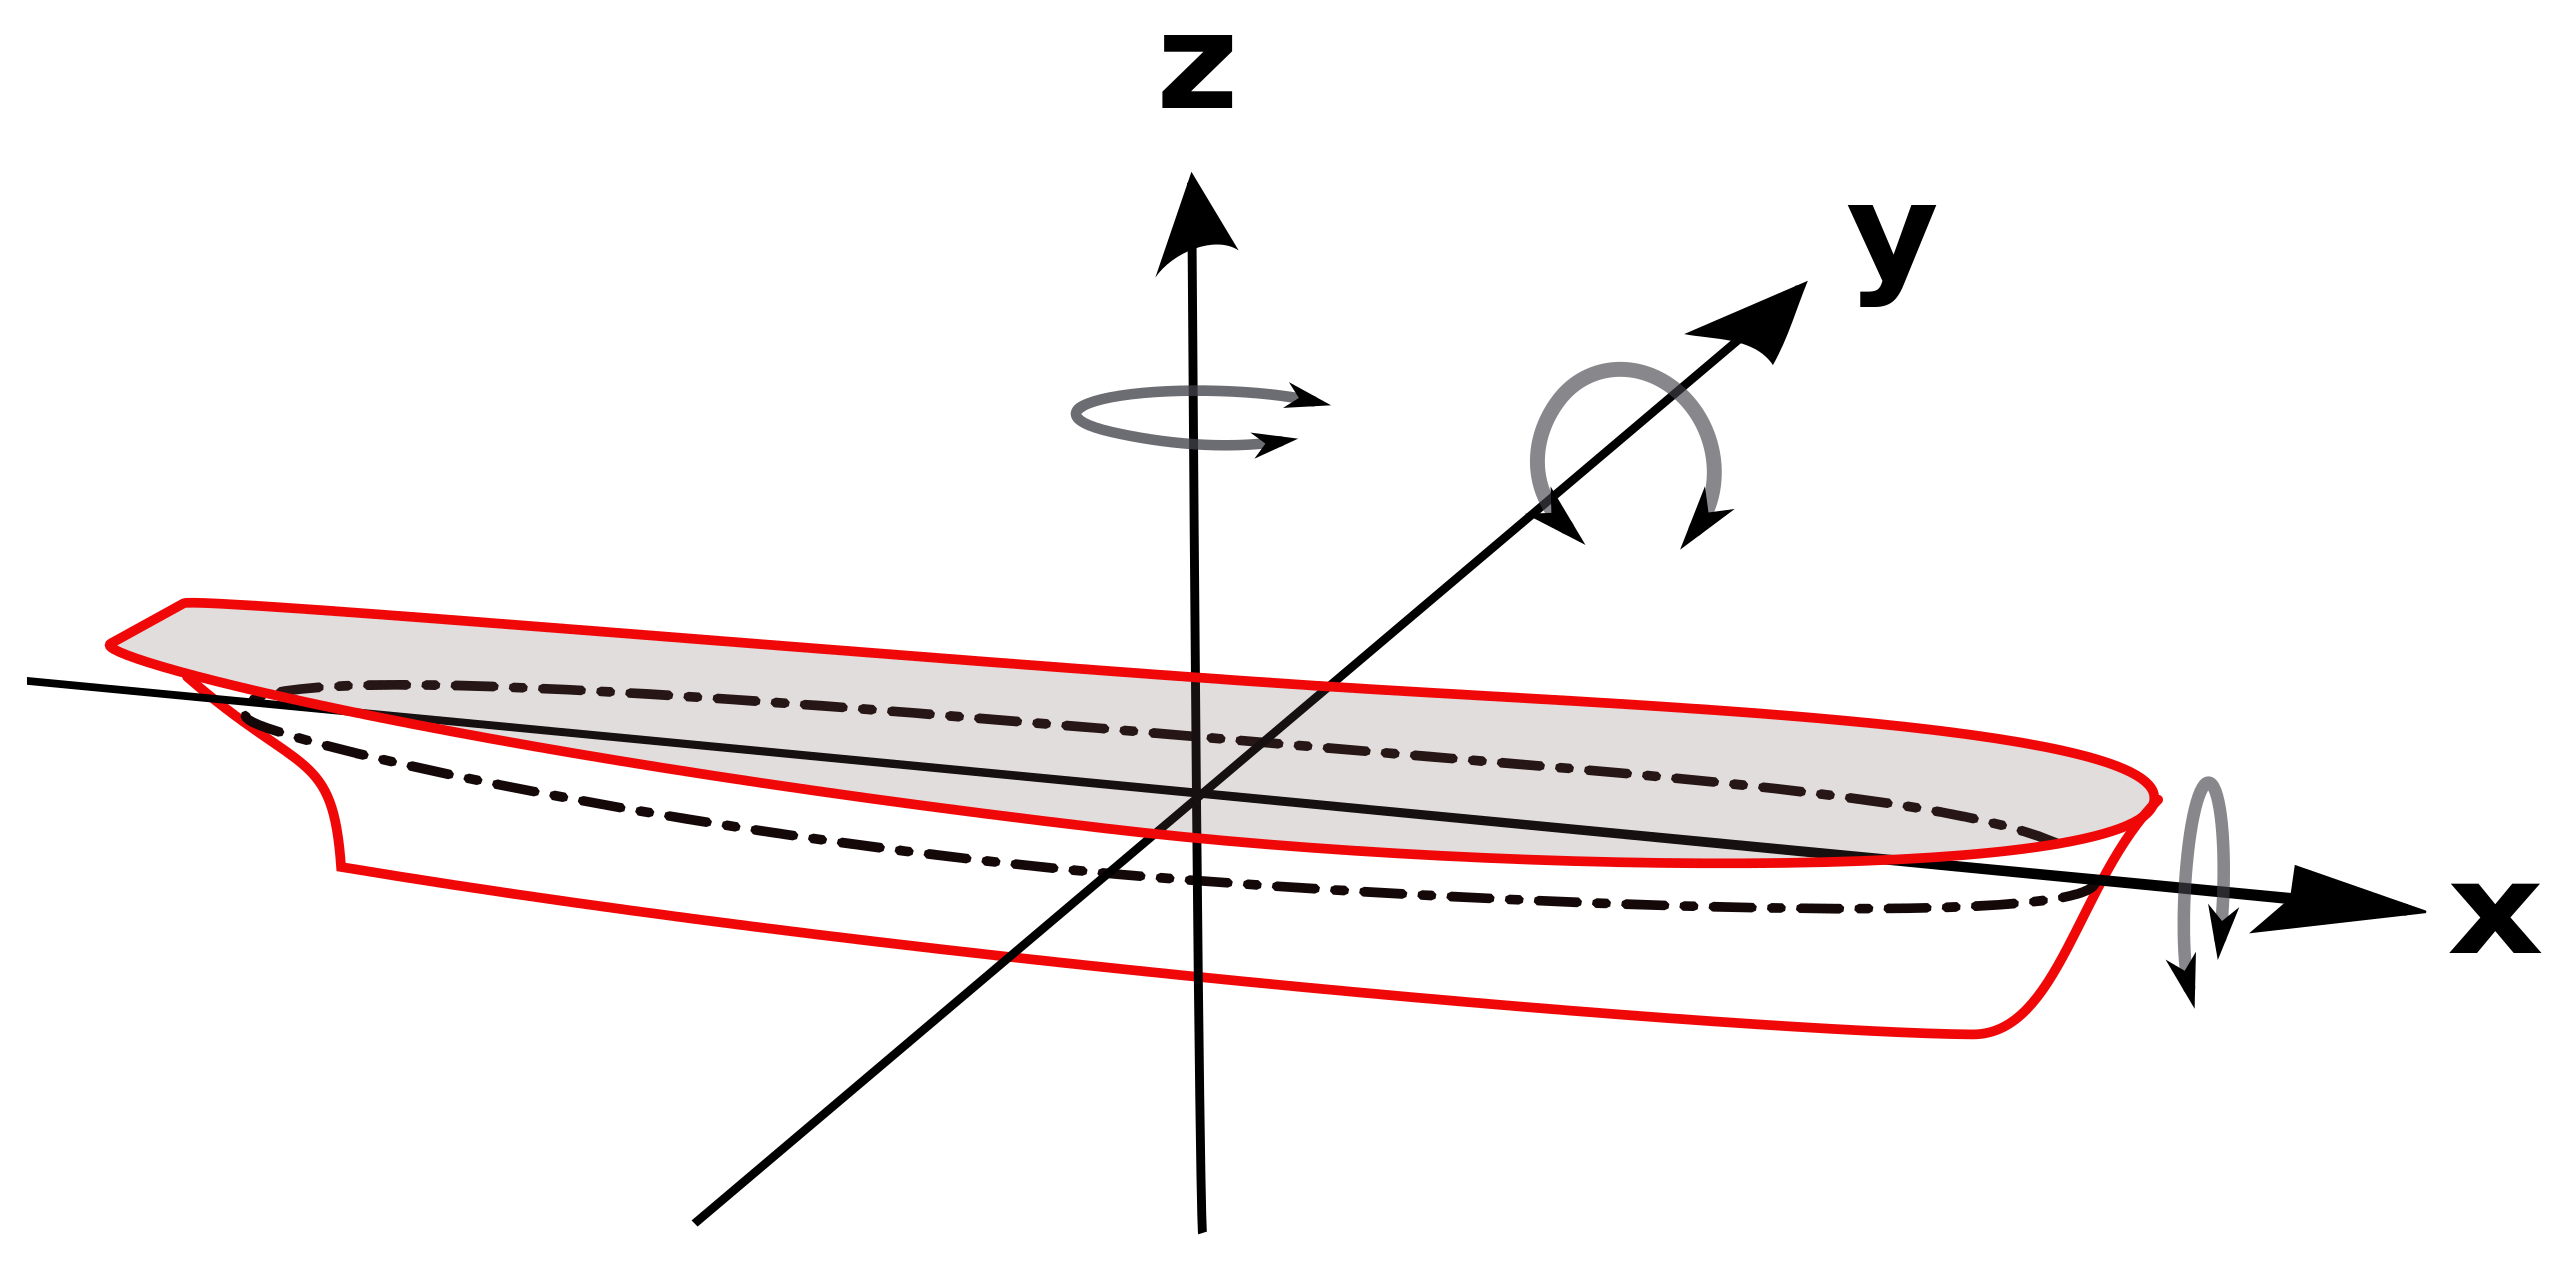
\includegraphics[width=0.5\linewidth]{assets/Achsen_Schiffsbewegung.svg.png}
    \caption{Krängung}
    \label{fig:enter-label}
\end{figure}
Die Stabilität eines Bootes wird durch die drei Parameter Gewichtsschwerpunkt, Auftriebsschwerpunkt (auch Form- oder Verdrängungsschwerpunkt genannt), sowie die sich aus ihnen ergebende sogeannte metazentrische Höhe bestimmt. \cite{noauthor_stabilitat_2023-1}  
\\Der Gewichtsschwerpunkt steht für die gesamte in einem Punkt konzentrierte nach unten wirkende Gewichtskraft des Bootes. Seine Lage innerhalb des Bootes  verändert sich bei einer Krängung nicht, solange alle Massen im Boot unverändert an ihrem Ort verharren. \\
Der Auftriebsschwerpunkt steht für die gesamte in einem Punkt konzentrierte nach oben wirkende Gewichtskraft des verdrängten Wassers. Seine Lage ändert sich bei einer Krängung, weil sich durch die Rumpfform auch die „Form“ des verdrängten Wassers ändert.\\
Bei aufrechter Schwimmlage des Schiffes liegt der Gewichtsschwerpunkt exakt vertikal über dem Auftriebsschwerpunkt. Führt ein äusserer Einfluss aber zu einer Krängung des Bootes, verändert sich die Lages des  stehen Gewichtsschwerpunkt auf der horizontalen Achse. Gewichtsschwerpunkt und Auftriebsschwerpunkt stehen  damit nicht mehr senkrecht übereinander. Dadurch entsteht ein aufrichtendes Drehmoment, welches das Boot bei Wegfall des krängenden Einflusses in seine Ausgangslage zurückführt. 
\begin{figure}
    \centering
    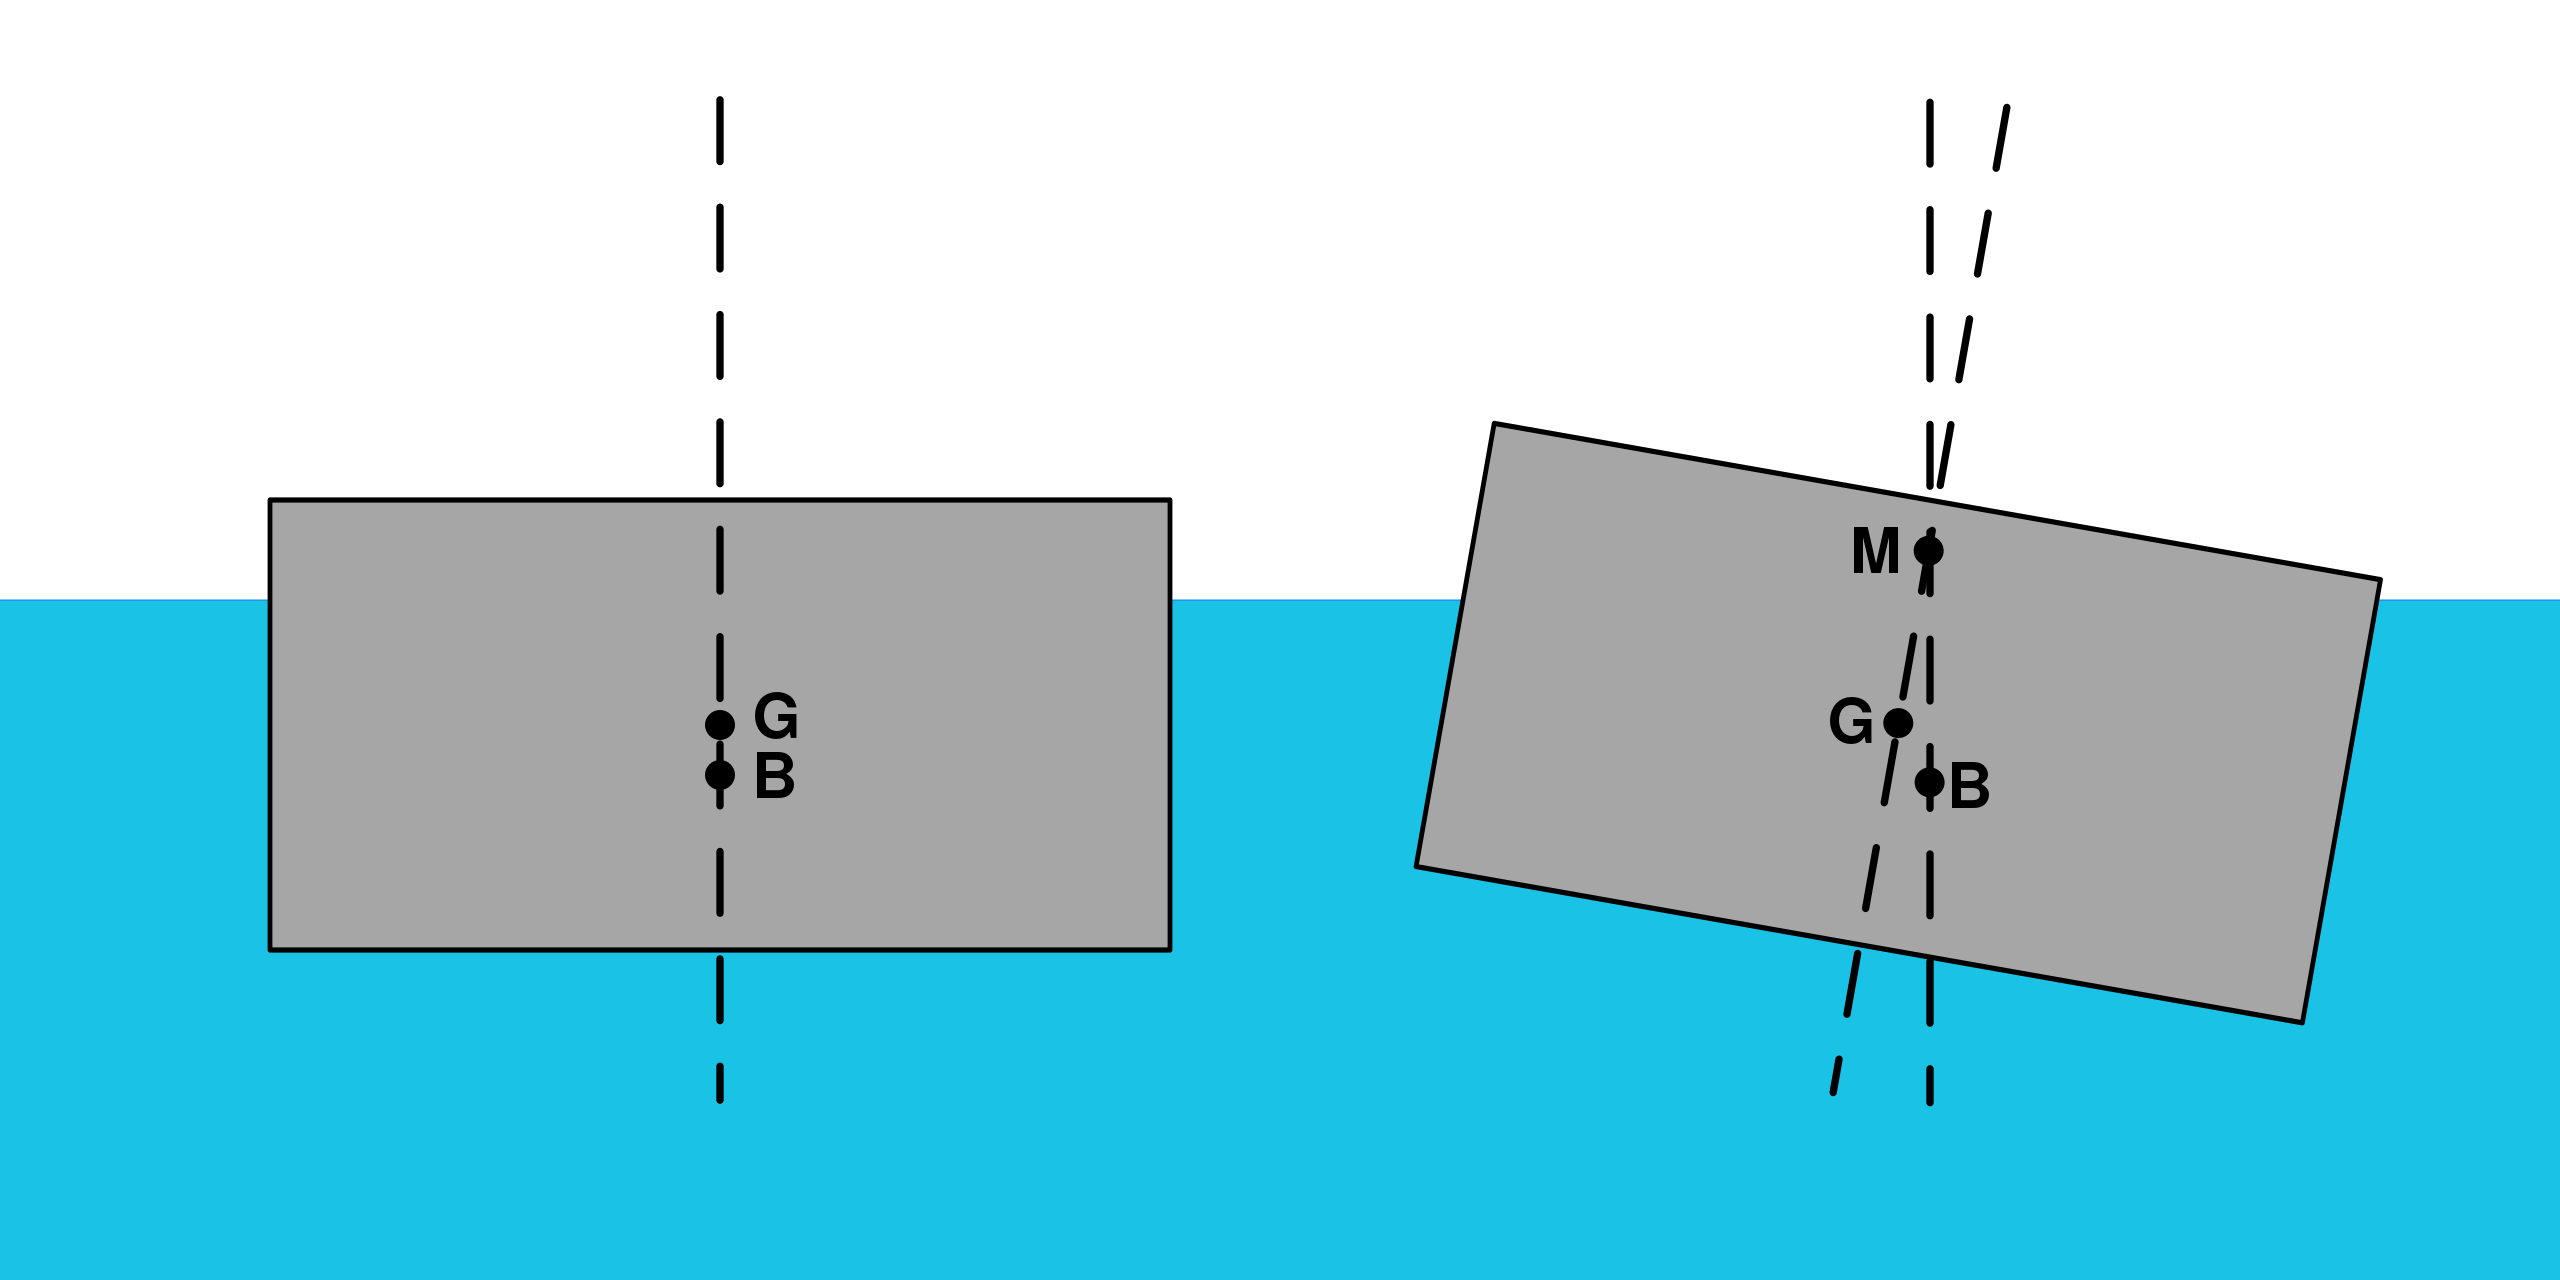
\includegraphics[width=0.5\linewidth]{Metacentriskhojd-svg.svg.png}
    \caption{Lage des Gewichtsschwerpunkt (G), Auftriebsschwerpunkt (B) und Metazentrum (M) bei aufrechtem, sowie gekrängtem Boot }
    \label{fig:enter-label}
\end{figure}
Zur Bewertung der Stabilität eines Schiffes müssen die folgenden drei Parameter bekannt sein: (i) die Anfangsstabilität (die sogeannte metazentrische Anfangshöhe), (ii) der Stabilitätsumfang und (iii) die Fläche unter der Hebelarmkurve. Die metazentrische Höhe ist der Parameter für den aufrichtenden Hebelarm. Mit dem Stabilitätsumfang wird die rechnerische Krängung des Schiffes in Winkelgraden bis zum Kenterpunkt bezeichnet und mit der Hebelarmkurve wird der jeweilige aufrichtende Hebelarm über den vollen Krängungsbereich bis zum Kenterpunkt des Bootes grafisch dargestellt. Der Hebelarm wächst bei zunehmender Krängung zunächst steil an, dann immer flacher an und wird bei noch stärkerer Krängung wieder geringer, bis er schließlich den Kenterpunkt (C) erreicht. Dieser liegt da, wo der Gewichtsschwerpunkt über den Auftriebsschwerpunkt hinauswandert. Mit der Fläche unter der Hebelarmkurve (A) lässt sich die Erfüllung der geplanten Mindeststabilität belegen.  \cite{noauthor_stabilitat_2023}

\begin{figure}
    \centering
    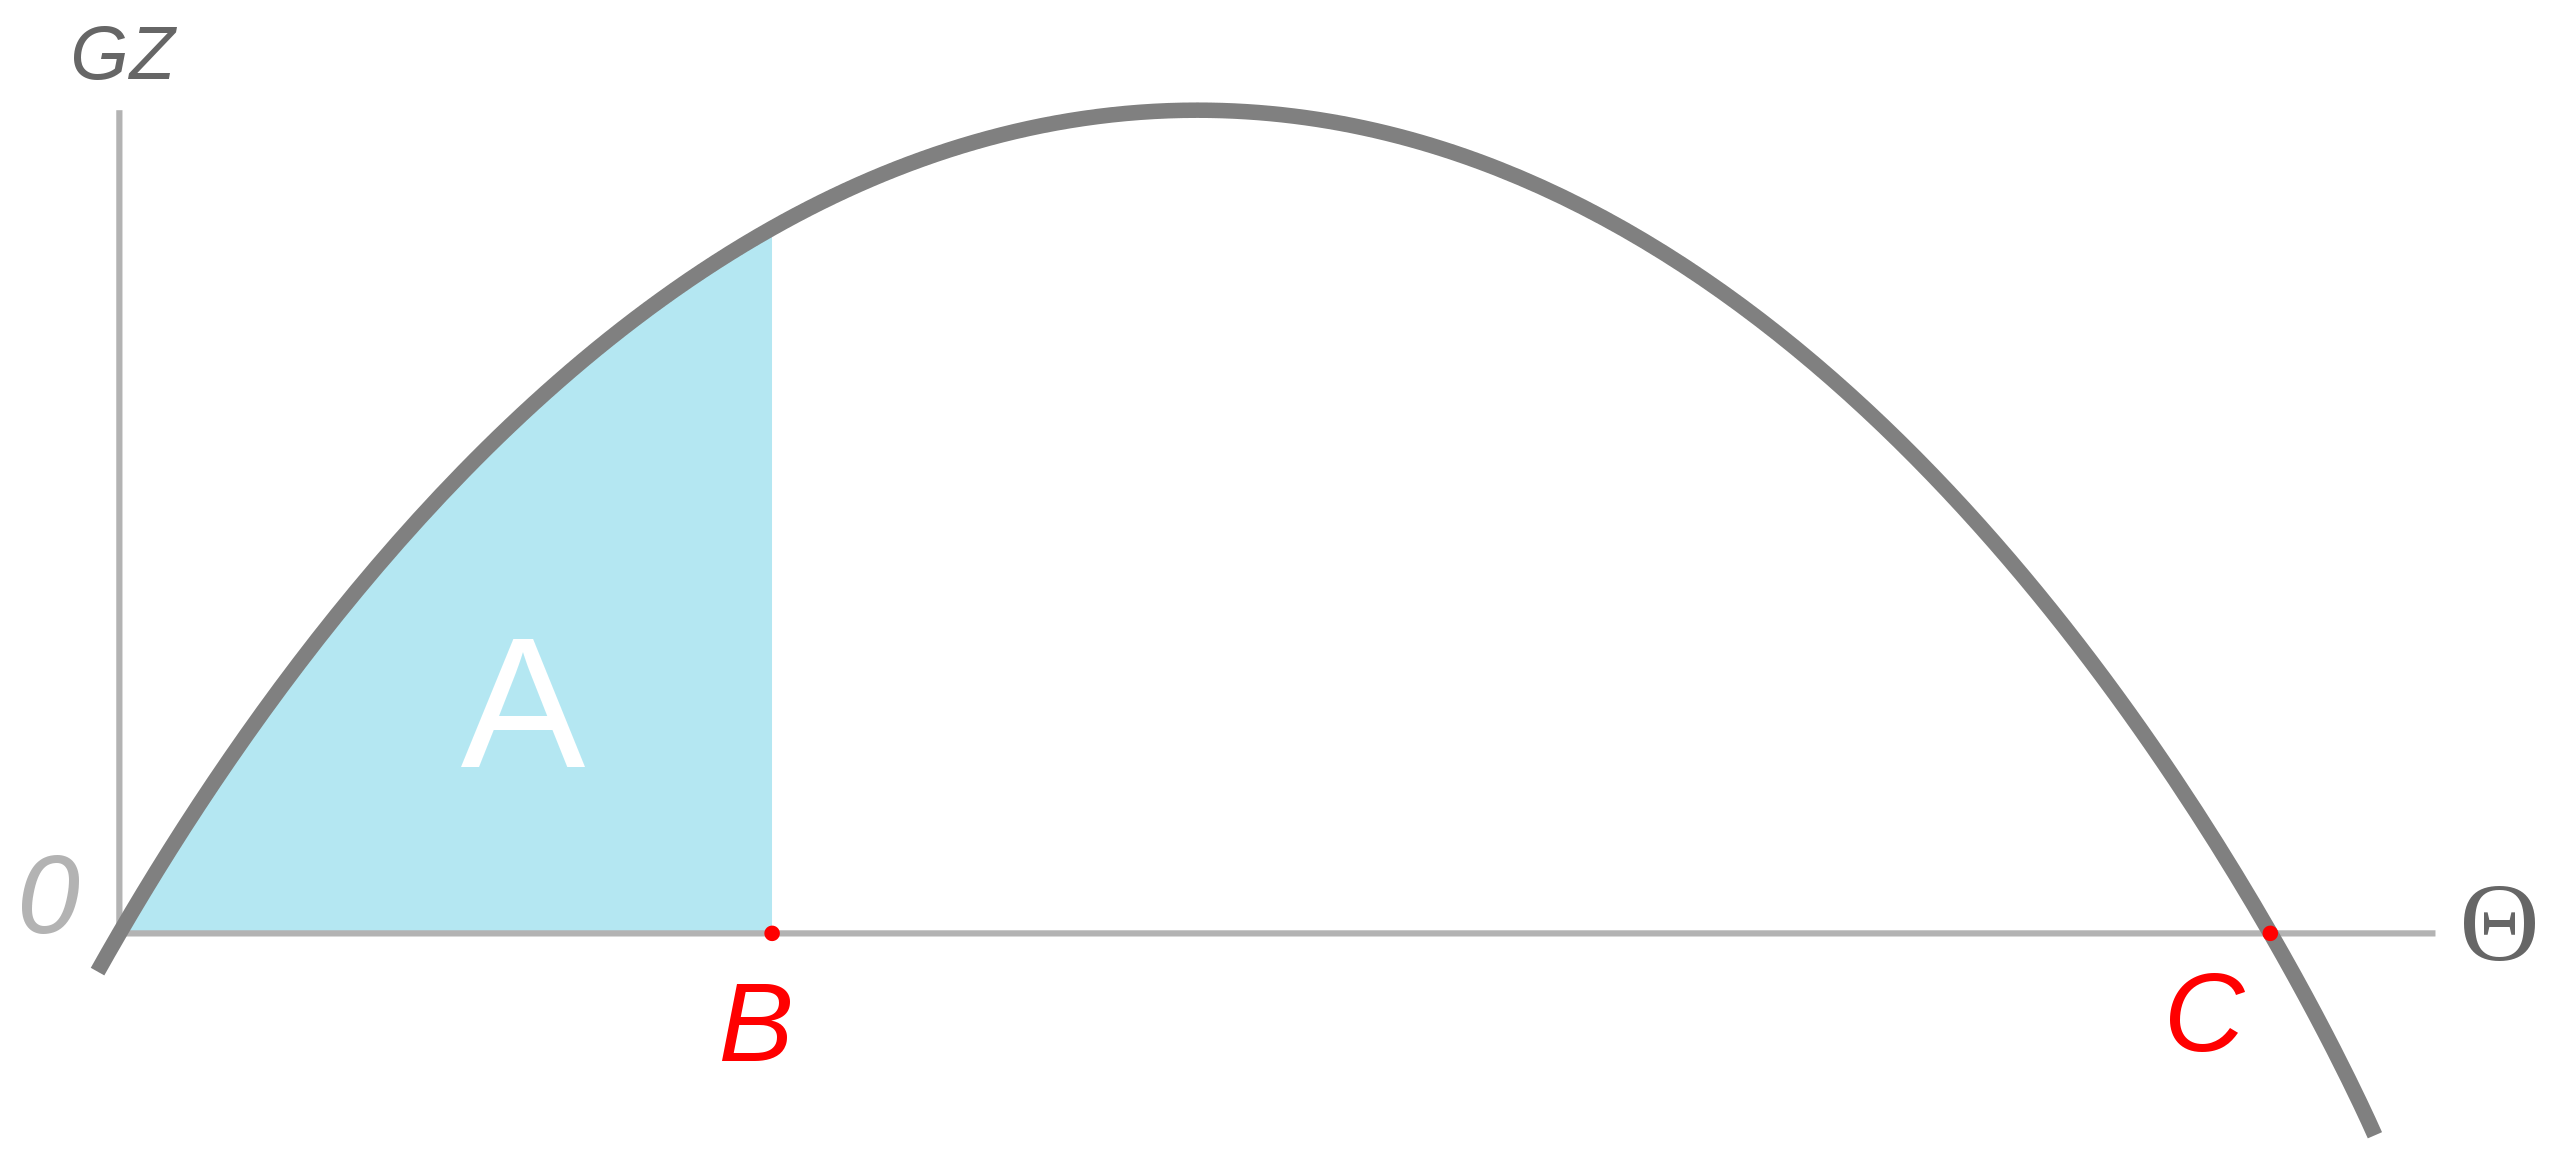
\includegraphics[width=0.5\linewidth]{Stability_curve_NT.svg.png}
    \caption{Hebelarmkurve}
    \label{fig:enter-label}
\end{figure}
Bei Segelbooten sind die Überlegungen zur Stabilität besonders wichtig, da sie mit ihren Segel für den Wind eine sehr grosse Angriffsfläche bieten. Ohne geeignete Gegenmassnahmen kippen sie schon bei geringen Windstärken um. Entscheidnd für die Stabilität eines Segelbootes sind dabei die Rumpfform und Gewichtsverteilung des Bootes. Die Krängung kann durch zwei Massnahmen wieder ausgeglichen und damit die Stabilität erhöht werden: 
\begin{itemize}
    \item Gewichtsstabilität – ein tief liegender Ballastkiel zwingt das Boot wieder in die aufrechte Lage (sogenanntes Stehaufmännchen-Prinzip).
    \item Formstabilität – die Form des Rumpfes begünstigt eine Rückkehr in die Ausgangslage.
\end{itemize}

\paragraph{Gewichtsstabilität}
Gewichtsstabilität durch Ballastkiel
Bei \href{https://de.wikipedia.org/wiki/Segelschiff}{Segelschiffen} wirkt ein \href{https://de.wikipedia.org/wiki/Kiel_(Schiffbau)}{Ballastkiel} als Gegengewicht der \href{https://de.wikipedia.org/wiki/Kr\%C3\%A4ngung}{Krängung} entgegen. Dieser enthält bis zu 50\% der Masse des Schiffes und bewirkt so ein aufrichtendes Moment. Eine gewisse Krängung unter Segeln – je nach Bauart des Schiffes von 20 bis 45° – ist bei diesen Schiffen normal und stellt keine Gefahr für das Schiff dar. Im untenstehenden Bild ist G der \textit{\href{https://de.wikipedia.org/wiki/Gewichtsschwerpunkt}{Gewichtsschwerpunkt}} (Schwerpunkt des Bootes) und A der \textit{\href{https://de.wikipedia.org/wiki/Formschwerpunkt}{Formschwerpunkt}} (Schwerpunkt der verdrängten Wassermasse). Für mechanische Betrachtungen kann man sich die Gewichtskräfte als im Punkt G vereinigt denken und die Auftriebskräfte als im Punkt A. Mit zunehmender Krängung wandert der Gewichtsschwerpunkt weiter nach außen und es erhöht sich damit das aufrichtende \href{https://de.wikipedia.org/wiki/Drehmoment}{Drehmoment}. Manche Segelschiffe richten sich daher selbst bei einer Krängung von mehr als 120° noch selbstständig wieder auf. Erst durch sehr hohen \href{https://de.wikipedia.org/wiki/Seegang}{Wellengang} können sie mit dem Kiel nach oben gedreht werden und gelten daher als \href{https://de.wikipedia.org/wiki/Kentern}{kentersicher}. Dringen allerdings größere Mengen Wasser ins Bootsinnere, sinken sie wegen des hohen Ballastgewichts. Verliert ein solcher Rumpf, beispielsweise nach einer Grundberührung, seinen Ballastkiel, so ist kaum mehr Stabilität vorhanden und das Kentern faktisch nicht mehr zu verhindern. 
\begin{figure}
    \centering
    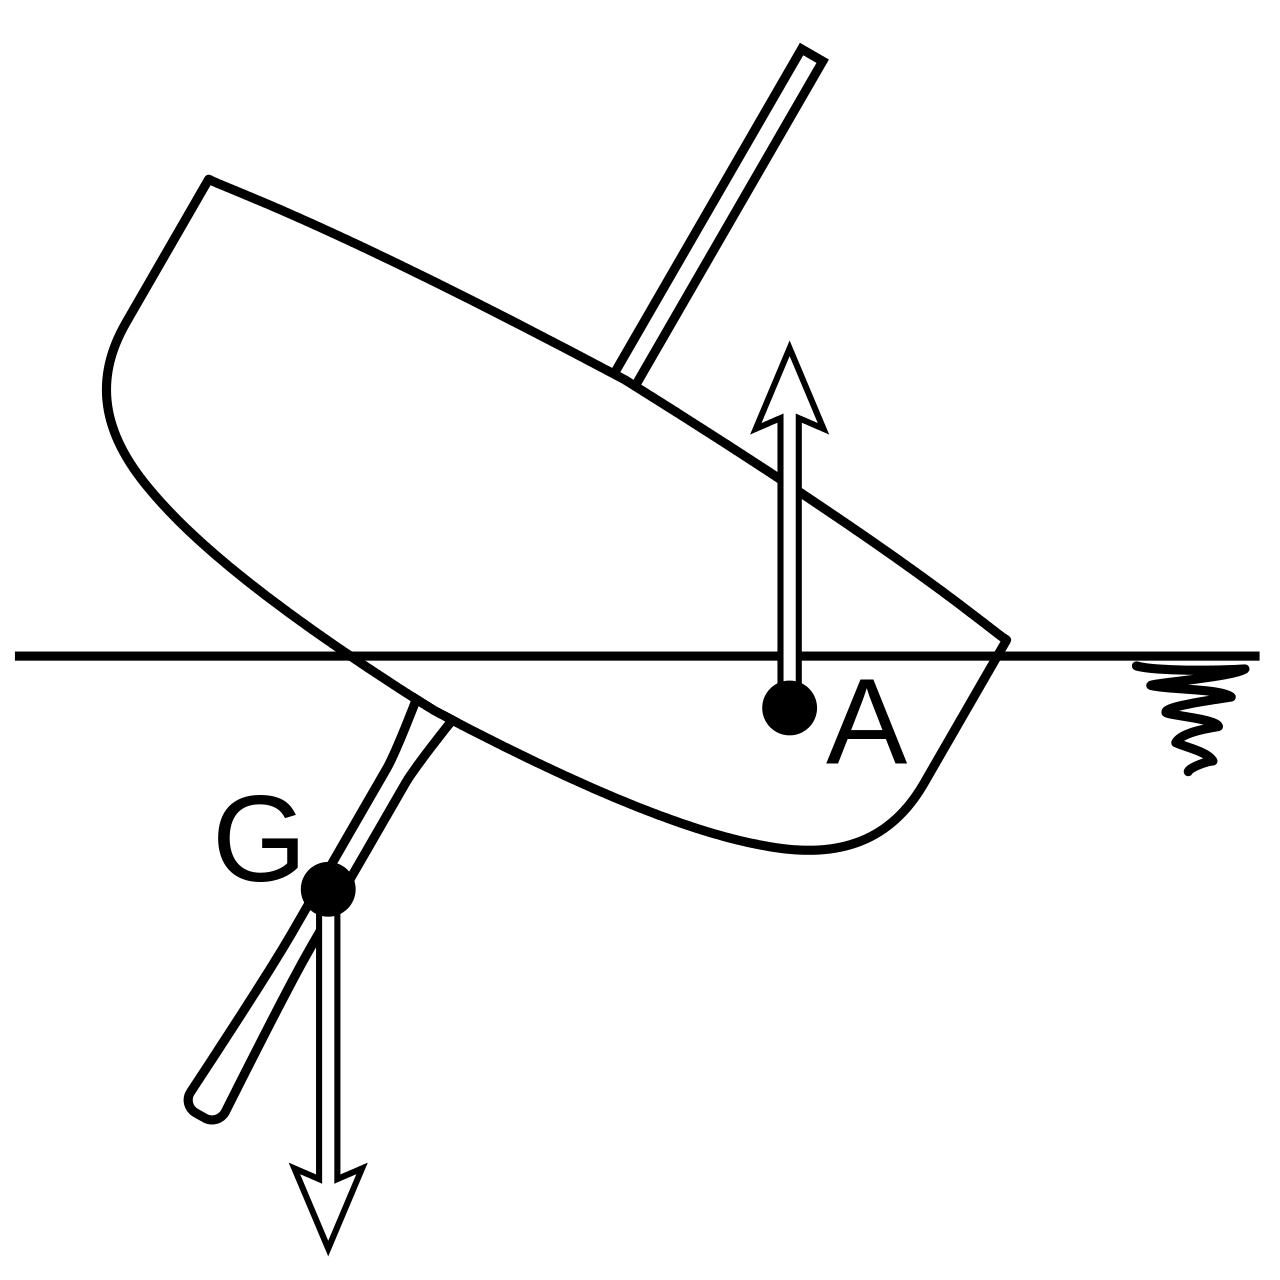
\includegraphics[width=0.5\linewidth]{Segeln_Gewichtsstabilitaet.svg.png}
    \caption{Gewichtsstabilität durch Ballastkiel }
    \label{fig:enter-label}
\end{figure}

\paragraph{Formstabilität}
Im Unterschied zu Kielyachten sind die meisten \href{https://de.wikipedia.org/wiki/Jolle}{Jollen} überwiegend formstabil. Das (meist ausklappbare) leichte Schwert einer Jolle hat keinen nennenswerten aufrichtenden Effekt. Auch \href{https://de.wikipedia.org/wiki/Segelkatamaran}{Katamarane} oder \href{https://de.wikipedia.org/wiki/Trimaran}{Trimarane} haben aufgrund ihrer Breite eine hohe Formstabilität. 
Im untenstehenden Bild ist G der Gewichtsschwerpunkt (Schwerpunkt des Bootes) und A der Formschwerpunkt (Schwerpunkt der verdrängten Wassermasse). In diesen Punkten kann man sich die Gewichts- bzw. Auftriebskräfte vereinigt denken. Für die Formstabilität ist die Lage von A ausschlaggebend. 

Bei aufrechter Lage des Bootes wird auf beiden Seiten des Rumpfes gleich viel Wasser verdrängt. A befindet sich dann mittig im Rumpfquerschnitt, es entsteht kein Drehmoment. Mit zunehmender Krängung (siehe Bild) wird Wasser vor allem auf einer Seite des Rumpfes verdrängt. Dadurch wandert A nach außen, es entsteht ein Drehmoment. Je breiter das Boot ist, desto weiter wandert A nach außen und desto stärker ist das aufrichtende Drehmoment. Wenn die Krängung zu groß wird, nimmt das Drehmoment allerdings wieder ab, weil dann der breite Rumpf gekippt ist und A wieder näher zur Mitte liegt. Eine leichte Krängung wird daher durch das kräftige aufrichtende Drehmoment kompensiert („Wasserwiderstand“), während eine zu starke Krängung zum Kentern des Bootes führt. Katamarane kentern, wenn die Krängung 90° erreicht.\textsuperscript{\href{https://de.wikipedia.org/wiki/Stabilit\%C3\%A4t_(Schiffsk\%C3\%B6rper)\#cite_note-Seemannschaft,_Seite_163-1}{[1]}} 

Es gibt sogar Beispiele für komplett formstabile Bootstypen mit negativer Anfangsstabilität. Diese haben im Ruhezustand keine aufrechte Schwimmlage. 
\begin{figure}
    \centering
    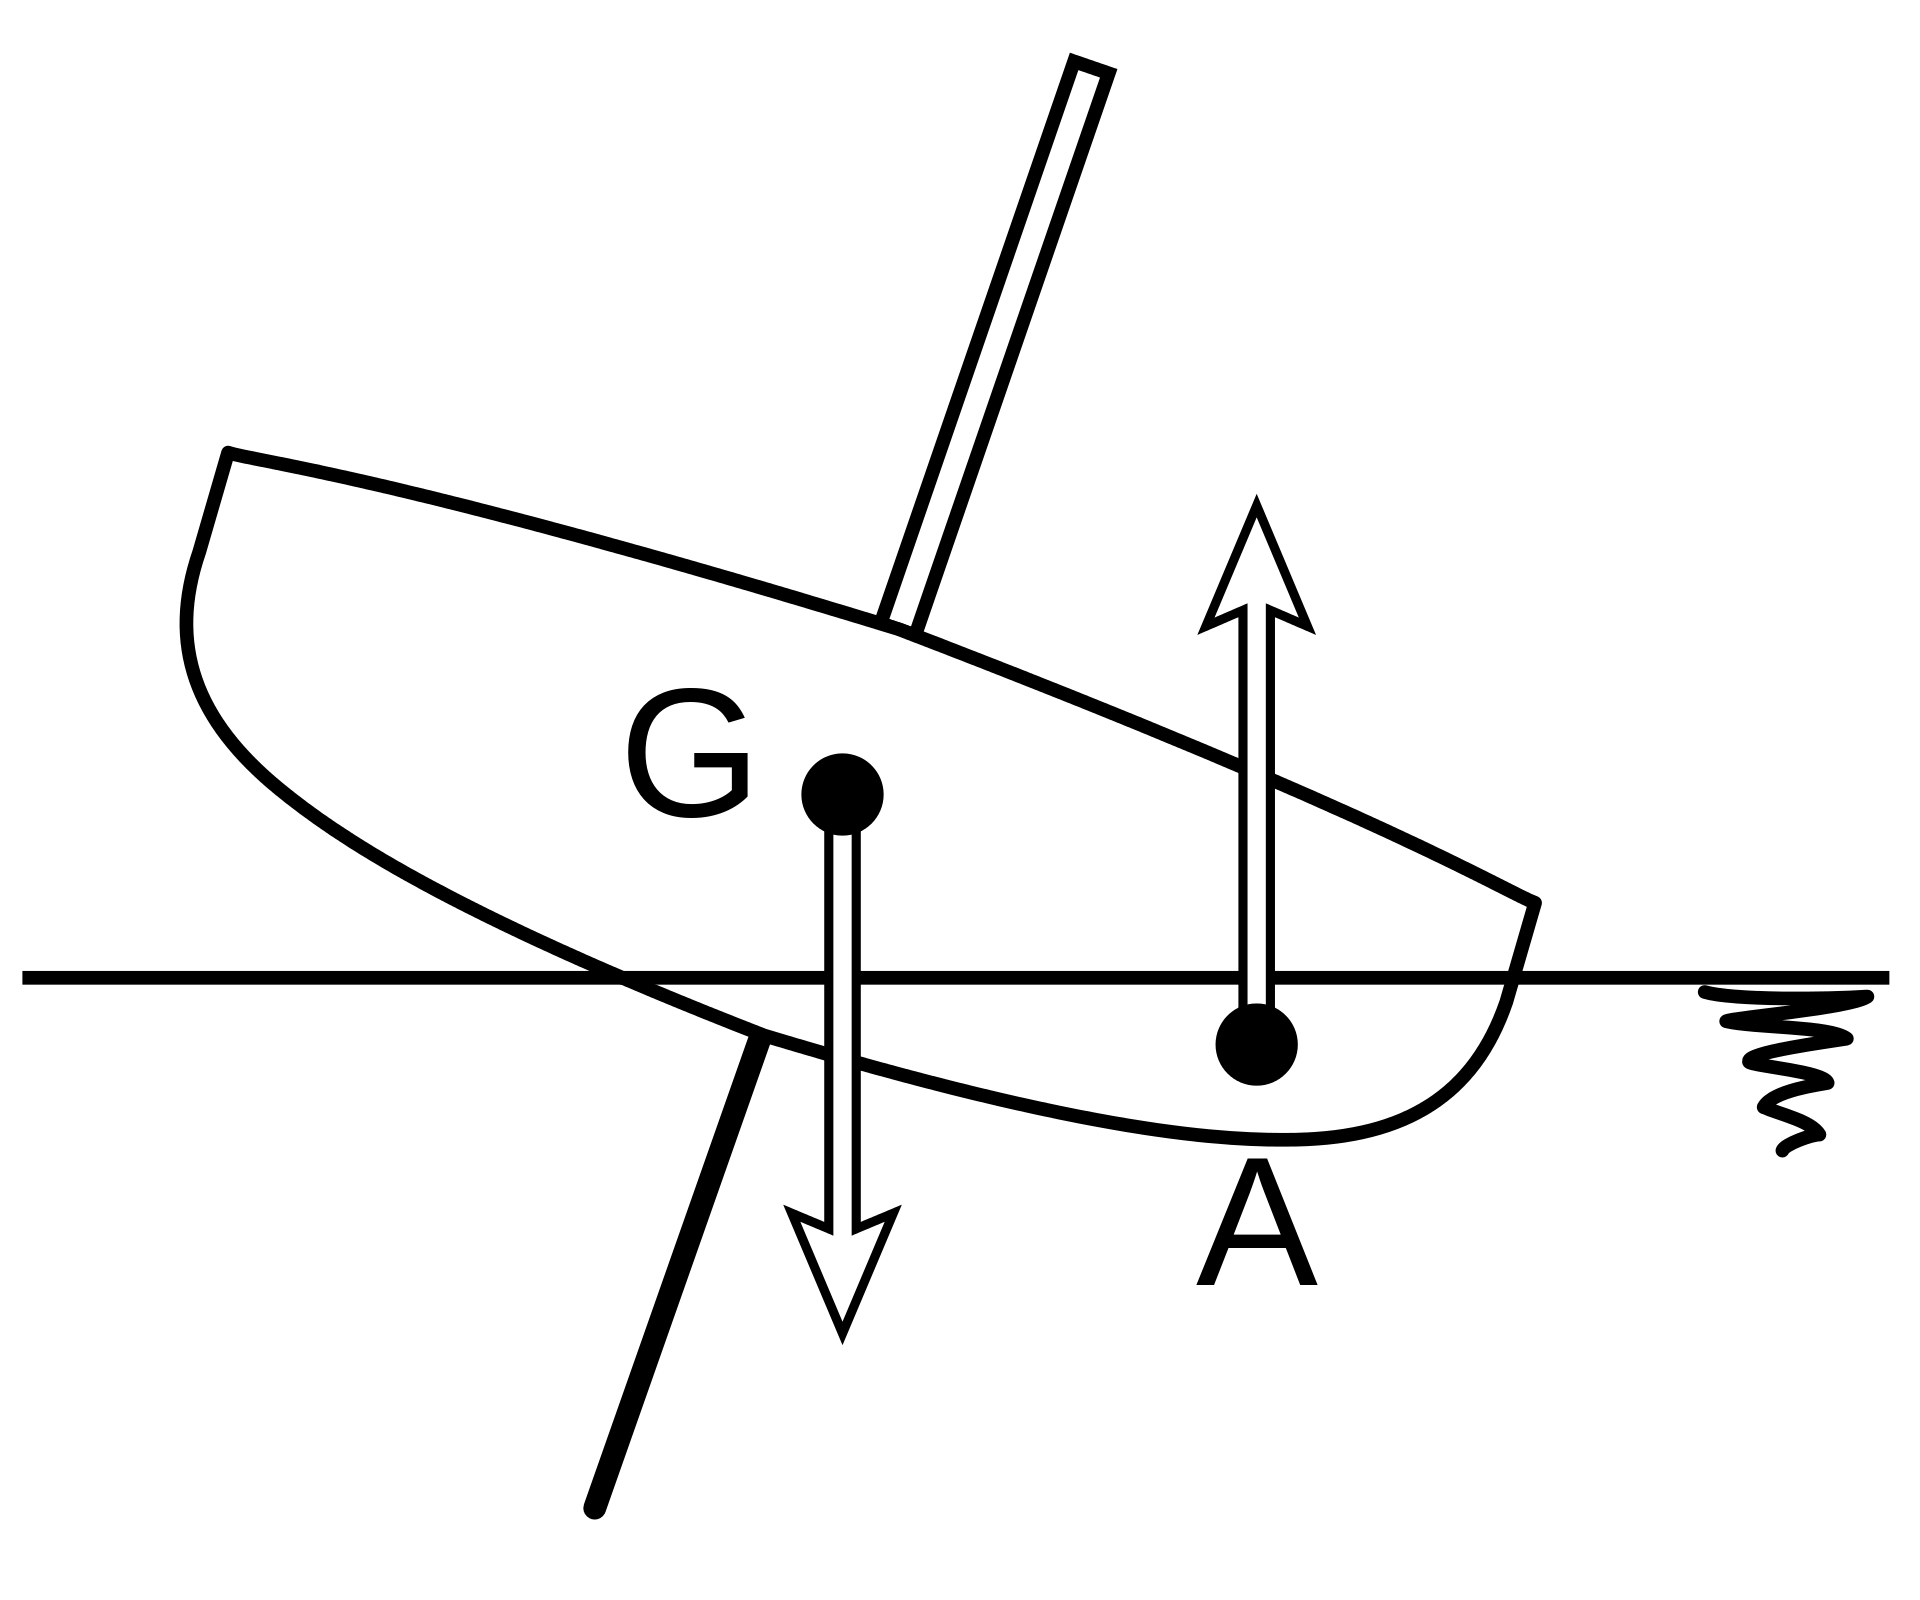
\includegraphics[width=0.5\linewidth]{Segeln_Formstabilitaet.svg.png}
    \caption{Formstabilität }
    \label{fig:enter-label}
\end{figure}

\paragraph{Gegenmaßnahmen bei großer Krängung}

Ein Segler hängt im Trapez, um den Katamaran auszubalancieren.Sowohl bei Kielbooten als auch bei Katamaranen oder Jollen kann die Krängung reduziert werden, indem sich die Crew „auf die hohe Kante setzt“, das heißt sich im \href{https://de.wikipedia.org/wiki/Luv_und_Lee}{Luv} an die Reling setzt, oder die Segelfläche reduziert wird (\href{https://de.wikipedia.org/wiki/Reffen}{Reffen}). Bei sportlich gesegelten \href{https://de.wikipedia.org/wiki/Jolle}{Jollen} hängt sich die Crew in ein \href{https://de.wikipedia.org/wiki/Trapez_(Segeln)}{Trapez}, um weiter nach Luv ausreiten zu können.\textsuperscript{\href{https://de.wikipedia.org/wiki/Stabilit\%C3\%A4t_(Schiffsk\%C3\%B6rper)\#cite_note-2}{[2]}} Beim sportlichen Segeln von Jollen kann eine Kenterung schon mal vorkommen. Sie sind im Gegenzug mit Schwimmkörpern ausgerüstet, so dass sie trotz Kenterung nicht sinken. Jollen sind dennoch nicht für die Hochsee geeignet und selbst gute Jollensegler werden bei angekündigten \href{https://de.wikipedia.org/wiki/Beaufort-Skala}{Windstärken} von mehr als 6 nicht mehr ablegen. 

Durch die Krängung wird automatisch die wirksame Segelfläche reduziert, auch die Form des Rumpfes bevorzugt einen bestimmten Krängungswinkel, bei dem das Schiff die höchste Geschwindigkeit erreichen kann. Daher wird durch starke Krängung das Schiff langsamer, zudem wird der Aufenthalt an Bord ungemütlicher. Auch steigt die Gefahr, dass es durch zu starke Krängung zu einem sogenannten \href{https://de.wikipedia.org/wiki/Sonnenschuss}{Sonnenschuss} kommt und das Schiff „aus dem Ruder läuft“\textsuperscript{\href{https://de.wikipedia.org/wiki/Stabilit\%C3\%A4t_(Schiffsk\%C3\%B6rper)\#cite_note-3}{[3]}} und „in den Wind schießt“.\textsuperscript{\href{https://de.wikipedia.org/wiki/Stabilit\%C3\%A4t_(Schiffsk\%C3\%B6rper)\#cite_note-4}{[4]}} Noch schlimmer ist es, wenn die Nock des \href{https://de.wikipedia.org/wiki/Baum_(Segeln)}{Großbaums} ins Wasser eintaucht, was zu schweren Schäden am \href{https://de.wikipedia.org/wiki/Takelage}{Rigg} führen kann. Daher kann durch rechtzeitiges Reffen – trotz verkleinerter Segelfläche – die Geschwindigkeit zunehmen. 

 Schwertboote haben \href{https://de.wikipedia.org/wiki/Formstabilit\%C3\%A4t}{formstabile} \href{https://de.wikipedia.org/wiki/Schiffsrumpf}{Rümpfe}. Ihr aufrichtendes \href{https://de.wikipedia.org/wiki/Drehmoment}{Drehmoment} wird nicht wie bei \href{https://de.wikipedia.org/wiki/Kielboot}{Kielbooten} durch einen \href{https://de.wikipedia.org/wiki/Kiel_(Schiffbau)\#Flossenkiel}{Ballastkiel}, sondern durch entsprechende Formgebung des Rumpfquerschnittes erreicht. Schwertboote sind im Allgemeinen relativ breit. Die \href{https://de.wikipedia.org/wiki/Schiffsmast}{Masthöhe} und die gefahrene \href{https://de.wikipedia.org/wiki/Segelfl\%C3\%A4che}{Segelfläche} sind im Verhältnis zur Rumpfgröße geringer als bei Kielbooten. Schwertboote besitzen bei leichter \href{https://de.wikipedia.org/wiki/Kr\%C3\%A4ngung}{Krängung} (Neigung) ein sehr hohes aufrichtendes Moment aufgrund ihrer Formstabilität. Dieses aufrichtende Moment nimmt jedoch mit zunehmender Krängung stark ab, so dass es zur \href{https://de.wikipedia.org/wiki/Kenterung}{Kenterung} kommen kann. Bei Kielbooten ist es umgekehrt, bei leichter Krängung ist das aufrichtende Moment gering und nimmt bei zunehmender Krängung zu, sodass sie kaum kentern können bzw. sich nach einer Kenterung von alleine wieder aufrichten.  (https://de.wikipedia.org/wiki/Schwertboot)


\section{Der Kiel bei Segelbooten} 

Bei Segelbooten erfüllt der Kiel zusätzlich zwei weitere Funktionen: 

\begin{enumerate}
    \item Er dient der Vergrößerung des \href{https://de.wikipedia.org/wiki/Lateralplan}{Lateralplans}, der die seitliche \href{https://de.wikipedia.org/wiki/Abdrift}{Abdrift} des Fahrzeugs vermindert und Auftrieb Richtung Luv erzeugt. Dies ermöglicht Segelfahrzeugen, hoch \href{https://de.wikipedia.org/wiki/Kurse_zum_Wind}{am Wind} zu segeln (schräg entgegen den Wind voranzukommen).
    \item Er sorgt für \href{https://de.wikipedia.org/wiki/Stabilit\%C3\%A4t_(Schiffsk\%C3\%B6rper)\#Gewichtsstabilit\%C3\%A4t}{Gewichtsstabilität}, die das Fahrzeug vor dem \href{https://de.wikipedia.org/wiki/Kentern}{Kentern} (Umkippen) bei starker \href{https://de.wikipedia.org/wiki/Kr\%C3\%A4ngung}{Krängung} (Schräglage) schützt.
\end{enumerate}
Für maximale Wirkung und gute Segeleigenschaften sollte das Kielgewicht so tief und so schwer wie möglich sein. Besonders in flachen Binnengewässern führt das allerdings zu erheblichen Einschränkungen bei der Wahl der möglichen Anlegehäfen, weshalb man hier vermehrt auf Hubkiele setzt oder anderweitige Kompromisse eingehen muss. Segelschiffe mit festem Kiel haben einen deutlich größeren \href{https://de.wikipedia.org/wiki/Tiefgang}{Tiefgang} als vergleichbare Motorschiffe. 

Schiffsmodelle aus über 50 Jahren Yachtbau. Gut erkennbar ist die Veränderung des Unterwasserschiffs über die Jahrzehnte (im Bild beispielhaft die diversen Yachten des deutschen Seglers \href{https://de.wikipedia.org/wiki/Hans-Otto_Sch\%C3\%BCmann}{Hans-Otto Schümann})Der hydrodynamische Auftrieb des Unterwasserschiffs wirkt in Richtung Luv und hält so das Schiff auf Kurs (siehe \href{https://de.wikipedia.org/wiki/Physik_des_Segelns}{Physik des Segelns}). Erkenntnisse aus der Strömungslehre ermöglichen es, effiziente Kielformen am Computer zu bestimmen. Die Wirksamkeit des Kiels als Auftriebsflosse ist in erster Näherung lediglich vom Quadrat des Tiefgangs, nicht aber von der Fläche des Unterwasserschiffs abhängig. Deshalb haben sich die Formen der Kiele in den letzten 50 Jahren deutlich verändert. Waren zu Beginn des modernen Yachtbaus noch lange Kiele üblich, sind sie heute sehr schmal und tief. 

 


\section{Wahl des Bootstypus}
\subsection{Wahl der Segelart}
Ausgangspunkt für die Wahl des Bootstypus für das vorliegende Projekt bildet der Entscheid über das zu verwendende Segel. Da sich das Segelboot autonom bewegen können muss, fällt dieser Entscheid leicht. Nur mit einem Festsegel lässt sich die Neigung flexibler Segel zu flattern vermeiden. 
Die Verwendung eines flexiblen Segels würde den Einbau einer sehr aufwändigen und auch fehleranfälligen Mechanik zur automatischen Trimmung des Segels mit Leinen und Rollen erfordern. 
Selbst wenn die Entwicklung einer Trimmmechanik gelingen würde, müsste das Segelboot zusätzlich in die Lage versetzt werden, ein loses (also ein flatterndes) oder zu stramme Segel selbständig zu erkennen und entsprechende Steuerbefehle an die Segeltrimmmechanik zu senden. Idealerweise müsste das Segelboot aber nicht nur jedes Abweichen von der idealen Segelform selbständig erkennen, sondern es müsste die negativen Auswirkung von Ruderbewegungen, Windböhen oder starkem Wellenschlag auf die ideale Segelform selbständig antizipieren können. Das würde erfordern, dass entweder direkt im Segel Sensoren verbaut würden oder dass das Segel optisch mittels einer oder mehrere Kameras erfasst würde. Aus diesen Daten würde dann in Echtzeit in einem ersten Schritt der Ist-Zustand des Segels berechnet, dieser in einem zweiten Schritt mit dem Idealzustand vergleichen, in einem dritten Schritt der Anpassungsbedarf berechnet, in einem vierten Schritt die notwendige Massnahme ermittelt (eine Verlängerung oder eine Verkürzug der Leinen (Schotten) und/oder ein Steuereingriff am Ruder) und in einem letzten Schritt der entsprechende Befehl an die Trimm- und/oder Steuermechanik übermittelt. Die Entwicklung einer solchen Trimmautomatik für eine flexibles Segel sprengt den Rahmen einer Maturaarbeit bei weitem, selbst wenn sie als selbständige Arbeit vorgesehen würde. 
Bei einem autonomen Segelboot dieser Klasse muss daher der Entscheid zwingend zugunsten eines Fixselgels lauten.
\subsection{Wahl der Rumpfzahl}
Ein Festsegel kann sowohl mit Einrumpfern als auch mit Mehrrumpfern eingesetz werden, womit der Entscheid über die Rumpfzahl nicht durch den Entscheid über die Segelart antizipiert wird.  
Für das vorliegende Projekt wird eine Einrumpfkonstruktion vorgezogen, da diese einfacher zu realisieren ist. Doppelrumpfboote verfügen über keinen Kiel und bieten damit keine Gewichtsstabilität. Nur Trimaranene können mit einem Kiel versehen werden, womit sie wie alle Kielboote Gewichts- und Formstabiltät bieten.  ist  Mehrrumpfboote zwar einen hohen Schutz gegen eine Kentern bieten, aber 

Festsegel Die erste und einfachste Kriterium für die Unterscheidung von verschiedenen Segelboot Typen ist die Anzahl der  Rümpfe. Wenn man sich ein Segelboot vorstellt, denkt man meist an ein Einrumpfboot, ein sogenanntes ”mono hull” Boot. Es gibt daneben aber auch Mehrrumpfboote (”multi hull”). Die berümtesten Vertreter dieses Rumpftypes sind die Kathamarane und die Trimarane.

Der Rumpf an sich kann jedoch auch innerhalb von einer von diesen Kategorien komplett unterschiedlich geformt sein.

\subsubsection{Segel}
Prinzipiell unterscheidet man zwischen zwei Segeltypen. Den Textilsegeln und den Hartsegel.
Textilsegel sind in der Segelwelt weit verbreitet, da sie viele Möglichkeiten zum Trimmen bieten,  vergleichseise einfach herzustellen und zu reparieren sind, eine flexible Veränderung der Segelfläche erlauben und bei Nichtgebrauch einfach verstaut werden können. Ausserdem sind sie deutlich günstiger als Hartsegel. 
\\
Für dieses Projekt werden dennoch Hartsegel vorgezogen, da dieser Segeltyp gerade für ein autonomes Segelboot bedeutende Vorteile aufweist. 


Weniger Komplex
da diese in der Regel einfach zu steuern sind und keine Trimmungen vorgenommen werden müssen. 
Bei einem Textilsegel, muss stets drauf geachtet werden, dass das Segel nicht flattert. Dieses Problem existiert bei einem Hartsegel schlicht und weg nicht.

\subsubsection{Kiel}
Kielboote vs. Jollen

Grundsätzlich muss entschieden werden, ob das Segelboot einen Kiel oder ein Schwert gegen den Abtrieb haben sollte. Ein Schwert und ein Kiel unterscheiden sich darin, dass ein Kiel eine gewisse Masse unten am Boot befestigt hat. Somit liegt der Massemittelpunkt tiefer und das Boot ist stabilier.
Ein Schwert hingegen funktioniert rein nach dem Prinzip des Wasserwiederstands, was das Boot daran hindert zu kippen.

 
Der Entwicklungsprozess des Kiels ist aufgrund der kaum vorhandenen Literatur zu dieser Frage sehr aufwendig. [???KANNST DU DIESE AUFFÜHREN????]\\ 

Die erste Fragestellung in diesem Bereich, ist ob ein Kiel oder ein Schwert verwendet werden soll. Der Unterschied zwischen Kiel und Schwert besteht darin, dass ein Kiel über ein beträchtliches Eigengewicht verfügt, das in der Regel durch die Verwendung von Balast  erreicht wird, während  ein Schwert lediglich den Wasserwiederstand nutzt und in der Regel aufholbar ist. Kiele werden hauptsächlich bei Jachten verwendet; Schwerter bei Jollen. 

 um das Boot aufrecht zu halten
Aufrichtendes Moment


Ein Kiel ist ein Teil des Rumpfes eines Bootes, der dafür sorgt, dass das Boot aufrecht bleibt und sich nicht auf die Seite legt. Er ist normalerweise das tiefste Teil des Bootes und erstreckt sich vom Bug bis zum Heck. Der Kiel ist sehr wichtig, um das Boot stabil zu halten und es steuerbar zu machen 

Neben der tragenden Funktion hat der Kiel bei Wasserfahrzeugen auch eine hydrodynamische Funktion. Er vergrößert den \href{http://en.wikipedia.org/wiki/de:Lateralplan}{Lateralplan} des Schiffes und erhöht damit seinen Querwiderstand im Wasser, verringert also die Abdrift durch Seitenwind. Dies ist für \href{https://www.modellbau-wiki.de/wiki/Segel}{Segelschiffe} besonders wichtig, um am Wind oder gegen den Wind (sogenanntes Kreuzen) zu segeln. Bei \href{https://www.modellbau-wiki.de/wiki/Segel}{Segelbooten} und kleinen Segelschiffen (z.B. \href{http://en.wikipedia.org/wiki/de:Ewer}{Ewer}) wird diese Funktion des Kiels durch \href{https://www.modellbau-wiki.de/wiki/Schwert_(Schiffbau)}{Schwerter} ergänzt, die in der Mitte des Kiels (Zentralschwert) oder seitlich des Rumpfes (Seitenschwert) angebracht sein können. Zudem ist der \textbf{Kiel} für die Gewichtsstabilität des Schiffes verantwortlich, verringert somit die \textit{Krängung} (Schräglage) und verhindert ein Kentern des Schiffes.  

Ein Kiel ist bei den meisten Wasserfahrzeugen zu finden, egal ob sie durch Wind oder Motor angetrieben werden. Es wird allgemein als eine feststehende Unterwasserverlängerung verstanden, die aus dem Boden eines Bootes herausragt, obwohl einige Versionen beweglich sind. Diese Verlängerung bietet Stabilität und widersteht seitlichen Bewegungen oder Drift. Seitwärtsbewegungen werden durch Wind oder Querströmungen verursacht und werden nicht nur durch Form und Tiefgang (Tiefe) einer Kielkonstruktion, sondern auch durch ihr Gewicht (oder Ballast) entgegengewirkt. 

Ein Schwert ist eine parallel zur Fahrtrichtung angebrachte senkrechte Platten und dient zur Verminderung der Abdrift beziehungsweise zur Umsetzung der Abdrift in Vortrieb. 
\\
Für dieses Boot wurde sich für ein Kiel entschieden, da es auf dem Boot keine möglichkeit gibt, Gewicht zu verschieben. Bei Jollen ist in der regel ein Segler auf dem Boot, welcher sehr viel mit seinem eigenen Körpergewicht steuert. Bei den meisten Jachten spielt das Körpergewicht der Segler keine oder nur eine untergeordnete Rolle.



\section{Entscheid für ein Kielboot}
Jollen, bzw. Schwertboote werden vorallem mit dem Eigengewicht des Seglers gesegelt. Seine Positiotion und seine Bewegungen Spigelen sich direkt in der Segelleistung wieder. Kentern gehört zum alltag von Jollnseglern genauso wie das Nasswerden.

Kielboote, bzw Yachten sind da etwas anders.Die Position der Mannschaft spielt keine bedeutende Rolle. Kielboote Kentern unter normalen Bedingungen nicht. Da ein Autonomes Segelboot über keine sich Bewegende Manschaft verfügt, noch irgendwelche Möglichkeiten zur verschiebung von Gewichten hat, ist ein Kielboot viel die einfachere Lösung.





%->	Baupläne werden generiert als Resultat



\section{Materialauswahl und -begründung }
% Turn around 
\subsection{Weichholz}
Die strukturell tragenden Elemente sind Hauptsächlich aus Holz gebaut. Dies hat den entscheidenden Vorteil der einfachen Verarbeitung. Ebenso hat Holz den Vorteil, dass es an sich schon schwimmt da es weniger Dicht als Wasser ist. Konkret werden zwei Holzarten verwedet. Zum einen Tannenholz und zum anderen Balasaholz. Das Tannenleimholz wird mit einer Stärke von 18mm verbaut und ist das kostengünstigste Holz was in dieser Kategorie im Baumarkt zu finden ist.
Alternativen zu Holz wären diverse Kunststoffe wie PLA, ABS, PETG, ect. welches durch 3D Druck geformt werden können. Jedoch wären die Kosten bei dieser Methode deutlich höher und eine gleiche Stabilität wie bei Holz zu erreichen wäre eine Herausforderung.
Ebenfalls möglich sind Rippenelemente aus Metallen, wie zum Beispiel Aluminium. Die Materialkosten sind bei Metallen jedoch weitaus höher und die Bearbeitung um ein vielfaches Komplizierter weshalb sich dagegen entschieden wurde.
\\
Für die Beplankung wird Balsaholz verwendet, da dieses sehr weich, biegsam und einfach zu be- und verarbeiten ist. Es ist im Modellbau weit verbreietet und in diversen Stärken verfügbar. In geringen Stärken von 1mm laässt es sich gut an die Form des Bootes anpassen.
% Balsaholz ABschnitt hinzufügen

\subsection{Fiberglas}
Da Balsaholz sehr porös ist, darf es unbehandelt nicht Wasser ausgesetzt werden. Selbst wenn es mit Lack gegen Feuchtigkeit geschützt wird, ist eine Balsaholzuhülle zu wenig robust, um die Aussenhülle des Bootes zu bilden.

Für die äussere Hülle werden Fiberglasmatten verwendet. Diese sorgen für eine stabile Hülle und schützen das Boot zusätzlich vor seitlichen Zusammenstössen. Ebenfalls sorgen sie dafür, dass das Boot dicht ist und kein Wasser hineinfliesst. Alternativ hätte man das Boot lediglich mit Epoxidharz abdichten können. Dies hätte aber dazu geführt, dass das Boot um ein vielfaches weniger stabil wäre. 

\section{Prozess der Konstruktion}
Bei der Konstruktion geht es um die Erstellung von Plänen. Das erfolgt bei komplexeren Konstruktionen immer computergestützt mittels sogenannten \ac{cad} Programmen. 

\subsection{Applikation}
Computer Aided Design (CAD) ist eine Form des technischen Zeichens, welches einem ermöglicht Modelle in Drei dimensionalen Raum zu gestalten. Somit lässt ist es verhältnissmässig einfach Technische Zeichnungen anzufertigen. Es gilt als eines der Wichtigsten Werkzeuge zur Planung von Maschienen und Geräten da sie so einfacher Vorstellbar sind und der Materialbedarf geplant werden kann. Die Konstruktion dieses Projekt beginnt mit dem erlernen von den Programmen Autodesk Inventor und Autodesk Fusion 360. 
Beide Programme verfolgen einen ähnlichen Ansatz und sind ähnlich Aufgebaut. Im Vergleich zu Inventor ist Fusion deutlich nutzerfreundlicher und ermöglicht es Projekte über eine Cloud einfacher zu speichern und von Unterwegs zu Bearbeiten. Die Programme von Autodesk wurden gewählt, da diese für den Persönlichen oder Bildungsgebrauch kostenlos sind. Open Source Programme wie FreeCAD wurden nicht gewählt, da diese weniger Intuitiv zum lernen sind und meist über weniger Funktionen verfügen. Programme welche als deutlich Leistungsstarker gelten wie NX Siemens oder Solidworks sind aufgrund der Lizensierungskosten für dieses Projekt nicht in Frage gekommen. 

\subsection{Konstruktionsvorgang des Rumpfes}
Da eine ebene Fläche für die Positionierung der Solarpanels benötigt wird, wird das Deck flach ausgelegt. Es bildet den Ausgangspunkt des Entwurfs. In einer Skizze wird die spätere Bootsform mithilfe gezeichnet. Da das Boot Wellen und Wetterbeständig sein sollte, muss das Boot über genügend Auftrieb verfügen. Daher wird eine Länge von 2.2m gewählt. \\
Für die maximale Breite werden 0.55m verwendet. Dies entspricht einem Viertel der Länge. Das Verhältnis zwischen der Länge und der Breite ist der Einflussreichste Faktor welcher über  Stabilität und die Manövrierfähigkeit. Ein Verhältnismässig Breites Boot ist deutlich stabiler als ein schmaleres, jedoch weniger Manövrierfähig. \cite{Seemannschaft} \\
\begin{figure}[H]
    \centering
    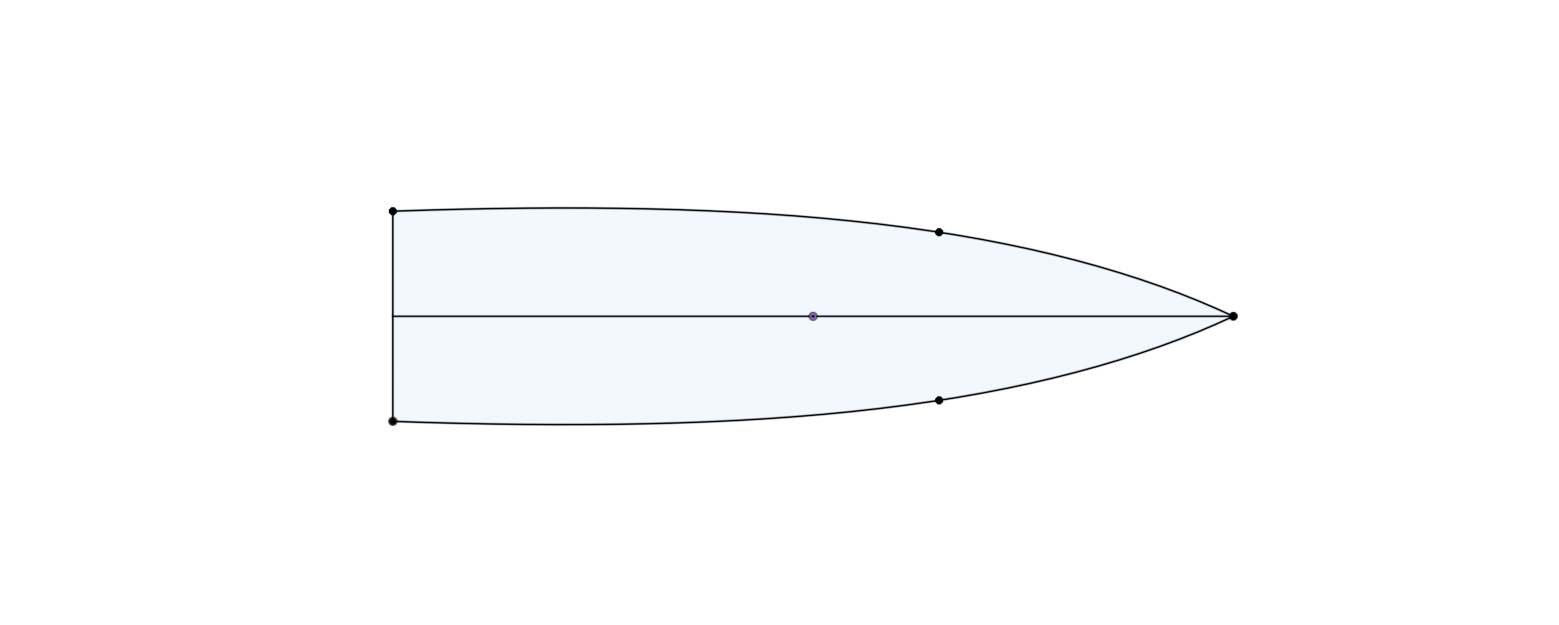
\includegraphics[width=1\linewidth]{assets/boot sketch top.png}
    \caption{Topansicht des Boots}
   
\end{figure}
In einem nächsten Schritt wird die Seitenansicht des Bootes konstruiert. Dieses Boot verfügt über einen angewinkelten Vorsteven und ein flaches Heck. Das Flache Heck wird gewählt, da die Befestigung des Ruders so am einfachsten ist und der Bug nach Hinten angewinkelt.

\begin{figure}[H]
    \centering
    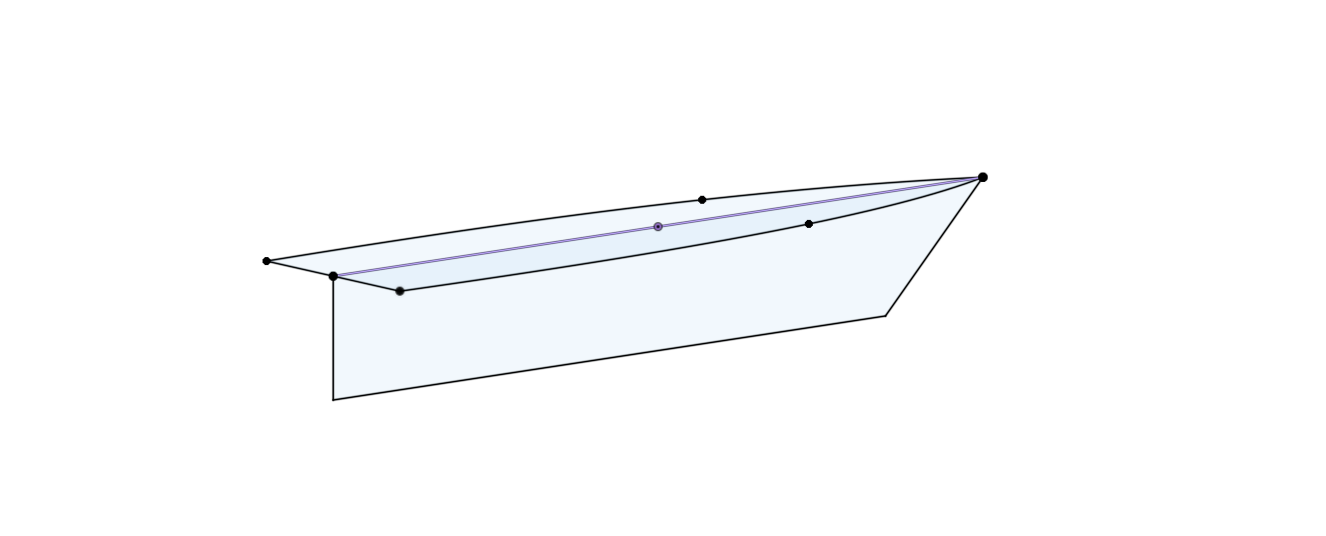
\includegraphics[width=1\linewidth]{assets/boot_skizze_2.png}
    \caption{Seitenansicht mit Steven}
    
\end{figure}

Als Heckform wurde eine leicht eingebeulte Form verwendet, welche dem Boot verhilft, senkrecht im Wasser zu stehen.

\begin{figure}[H]
    \centering
    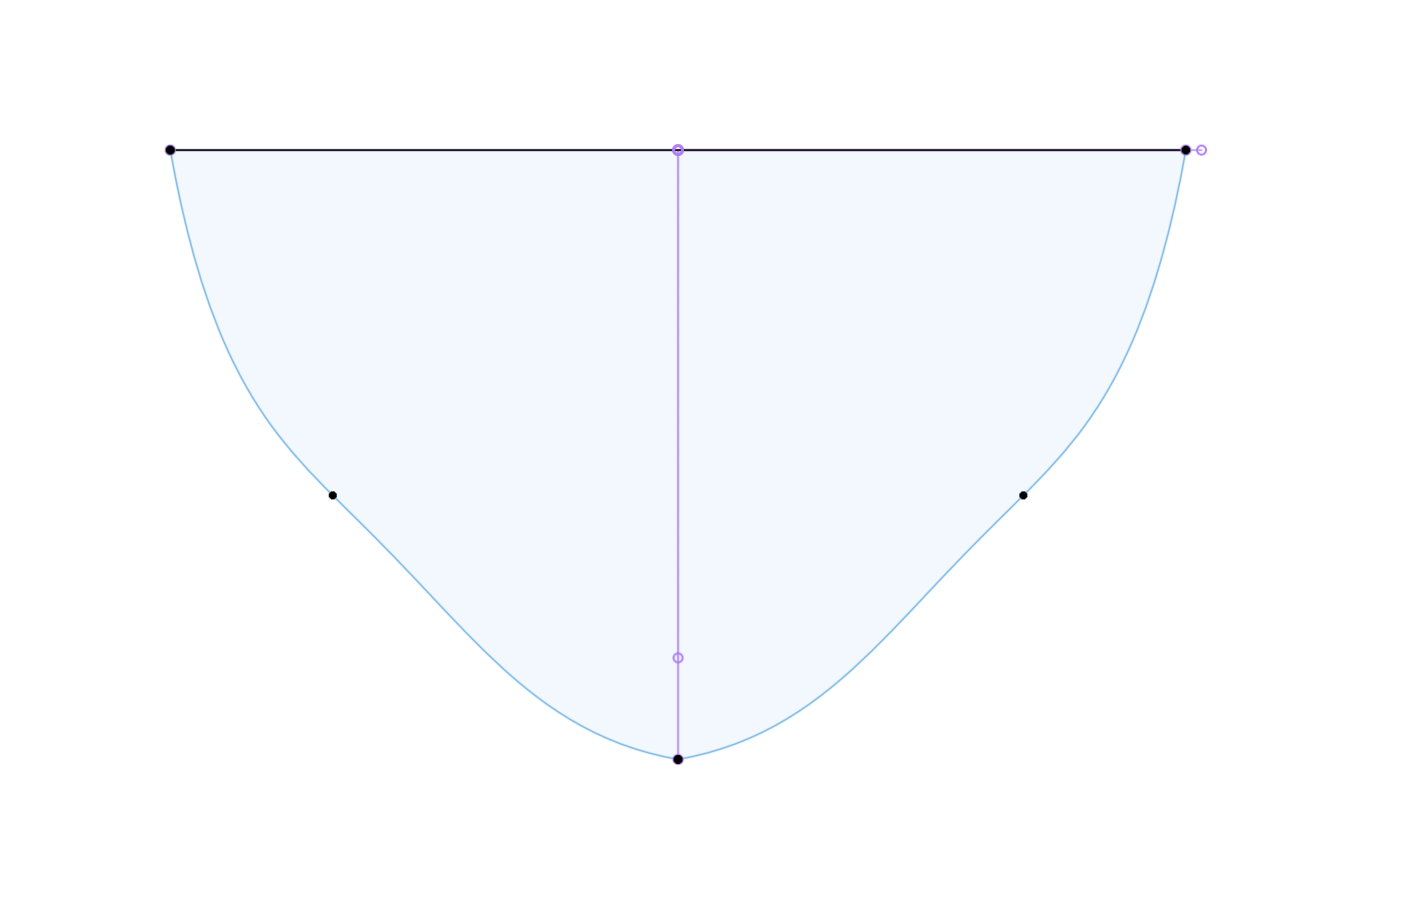
\includegraphics[width=0.6\linewidth]{assets/Heck_boot.png}
    \caption{Heckansicht}
   
\end{figure}

Mit dem Erhebungswerkzeug (Loft Tool) wird im Anschluss aus den Skizzen ein Körper berechnet. Unten am Rumpf wird zudem eine Begradigung hinzugefügt welche es ermöglicht den Kiel senkrecht am Boot zu montieren.
\begin{figure}[H]
    \centering
    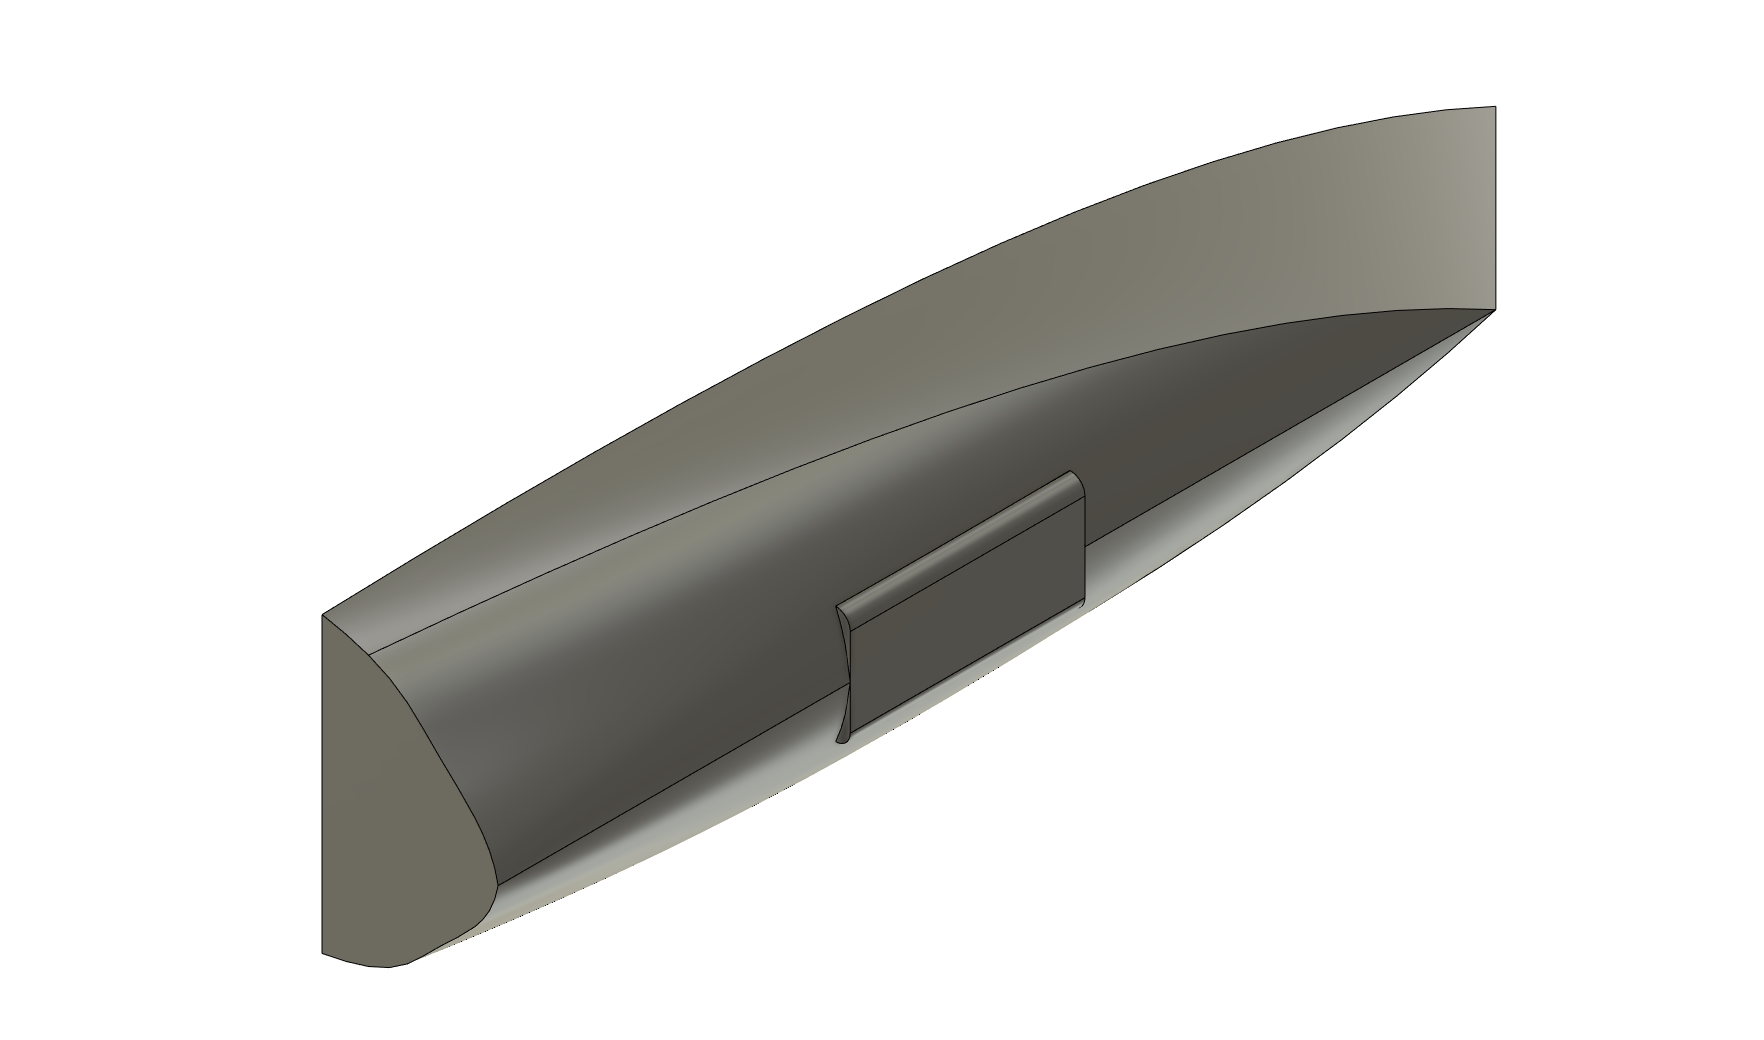
\includegraphics[width=0.75\linewidth]{assets/kielbefestigung2image.png}
    \caption{Fläche zur Montierung es Kiels}
    \label{fig:enter-label}
\end{figure}

Im Anschluss wird die Form mit einer Randstärke von 4 cm innen ausgehölt. 
\begin{figure}[H]
    \centering
    \includegraphics[width=1\linewidth]{assets/Hohlkörper.png}
    \caption{Schnittbild Hohlkörper}

\end{figure}
Im nächsten Schritt wird der bereits ausgehöhlte Körper auf zwölf Spanten mit einem einheitlichem Abstand 14 cm reduziert. Die Spanten haben eine Stärke von 18 mm. Die Masse der Spanten verjüngen sich von der Mitte zum Bug und Heck hin.

\begin{figure}[H]
    \centering
    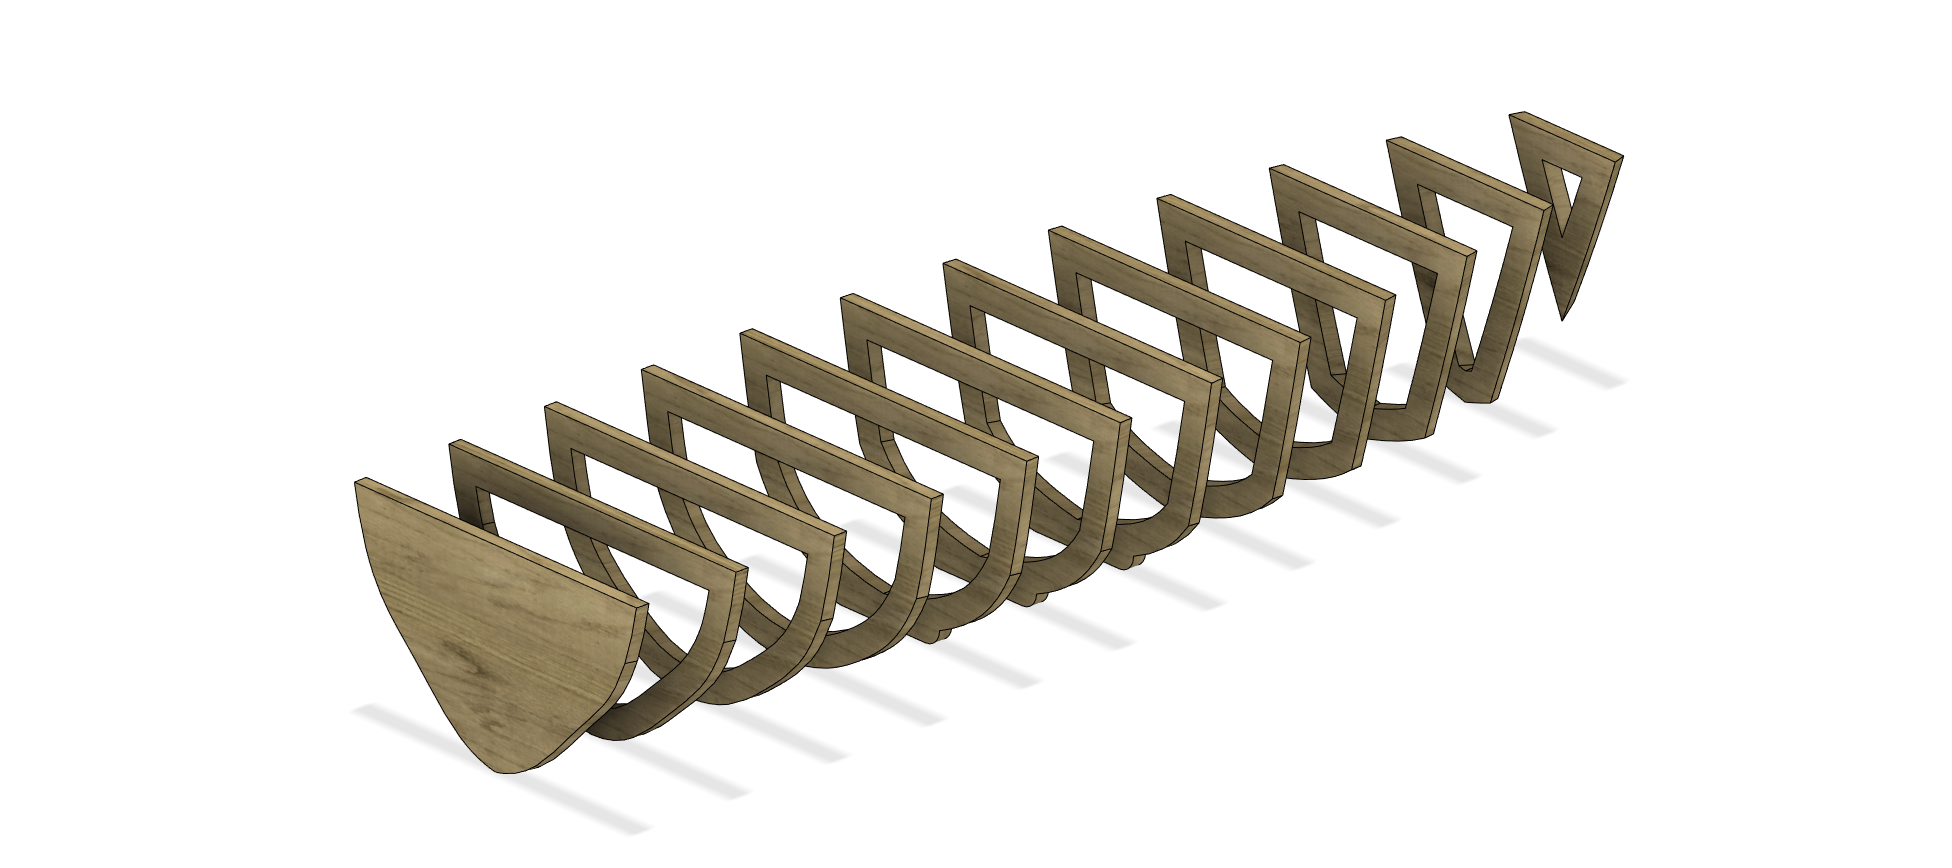
\includegraphics[width=1\linewidth]{assets/rippen_cad.png}
    \caption{Spantenansicht}
    
\end{figure}
Die letzte Spannte, der Achtersteven genannt wir, ist nicht hohl, weil sie sich am Ende des Hohlkörpers befindet und diesen abschliesst.  \\

Mit Ausnahme der Spanten 5, 6 und 7 laufen die Spanten unten spitz zu. Die Spanten 5, 6 und 7 sehen einen flachen Boden von  ??????? cm vor, der dazu dient, später den Kiel des Bootes sicher befestigen. 

Bild von Spanten 5, 6, und 7unten einfügen !!!!!!!!

Der Bug des Bootes läuft spitz zu. Diese Form der Spitze ist in Holz schwierig zu bauen. Es wird daher auf die klassische Konstruktion mit einer Bugspante verzichtet. An ihrer Stelle wird die gesamte Spitze im 3D Druckverfahren aus Kunststoff als ein einziges Werkstück gedruckt. Es wird mit der vordersten Spante verklebt. Der Bugspitz ist nicht in Massivbauweise vorgesehen, sondern als Hohlkörper vorgesehen.
\begin{figure}[H]
    \centering
    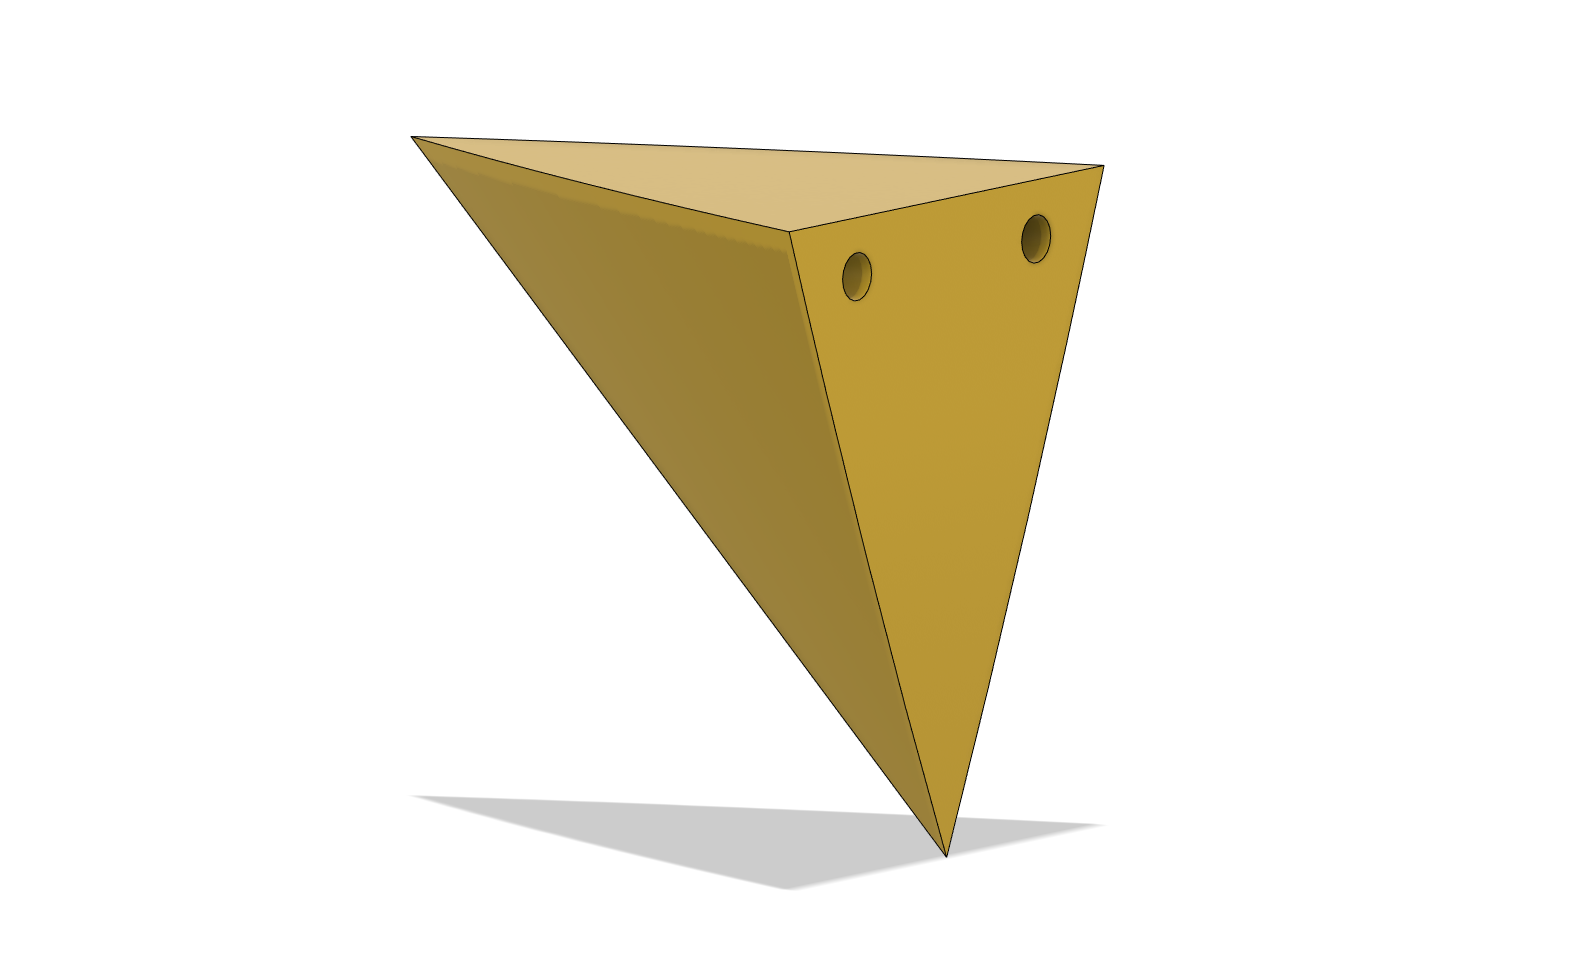
\includegraphics[width=0.8\linewidth]{assets/bug_spitz.png}
 \caption{Bugspitz}
    
\end{figure}
Die meisten Boote und Schiffe verfügen über einen mittschiffs im Boden angebrachten Längsverband, der das Rückgrad des Bootes bildet. An ihm sind die querstabilisierenden Spanten befestigt. Dieser Längsverband bildet zusammen mit einer vertikalen Unterwasserverlängerung den Kiel und mündet am Anfang und Ende in den Steven. 
\\
Da für die vorliegende Konstruktion ein Flachdeck vorgesehen ist, der Boden des Schiffskörpers aber gewölbt ist, wird von dieser klassischen Kielkonstruktionsweise abgewichen. Die Längsverbindung der Spanten wird nicht am Boden des Schiffes, sondern direkt unter dem Deck vorgesehen. Sie besteht auch nicht aus einem  einem einzigen mittschiffs angebrachten Längsverband, sondern aus zwei Längsverbänden, die in einem  Abstand von 10 cm von der Mittelachse parallel über die ganze Bootslänge horizontal angebracht werden. Sie bestehen aus zwei Alluminiumröhren mit einem Durchmesser von je 16 mm. Die beiden Röhren werden durch die Spanten geführt, in welchen im oberen Holm je zwei runde Löcher im Abstand von 10 cm gebohrt werden. Am vorderen Ende des Bootes werden die beiden Röhren in zwei dafür vorgesehene Hohlöffnungen des gedruckten Bugspitzes geführt und verklebt.
\\
Diese Konstruktion ist viel einfacher zu bauen als ein klassischer Kielaufbau.  Sie ist bei  bemannten Booten nicht verbreitet, weil die beiden Längsverbindungen direkt unter dem Deck dem Einbau eines Cockpits im Weg stehen würden. Möglich wäre allein das Cockpit auf dem Deck aufzubauen, was sowohl die Stabilität als auch den Komfort stark beeinträchtigen würde. Auch ein  Zugang zu einer Kajüte würde verunmöglicht. 
\begin{figure}[H]
    \centering
    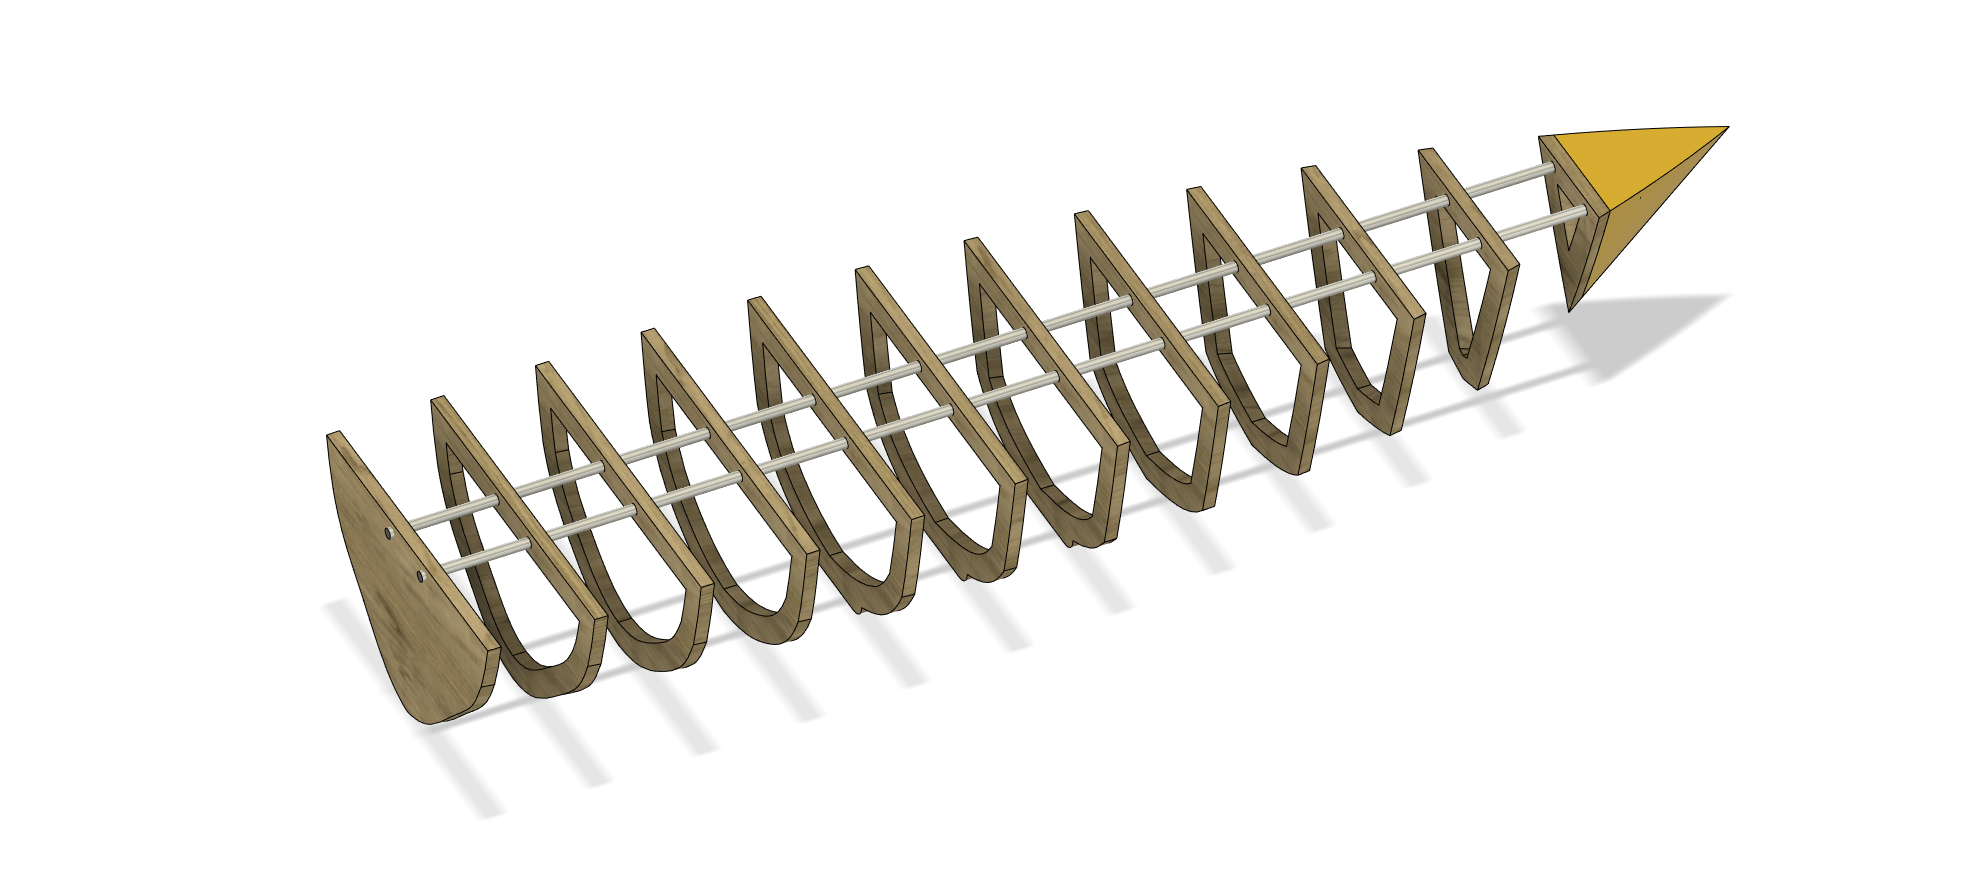
\includegraphics[width=1\linewidth]{assets/full_skellet.png}
    \caption{Abbild der Spanten und des Spitzes in Verbindung}
    
\end{figure}

%\begin{figure}[H]
%  \centering
%  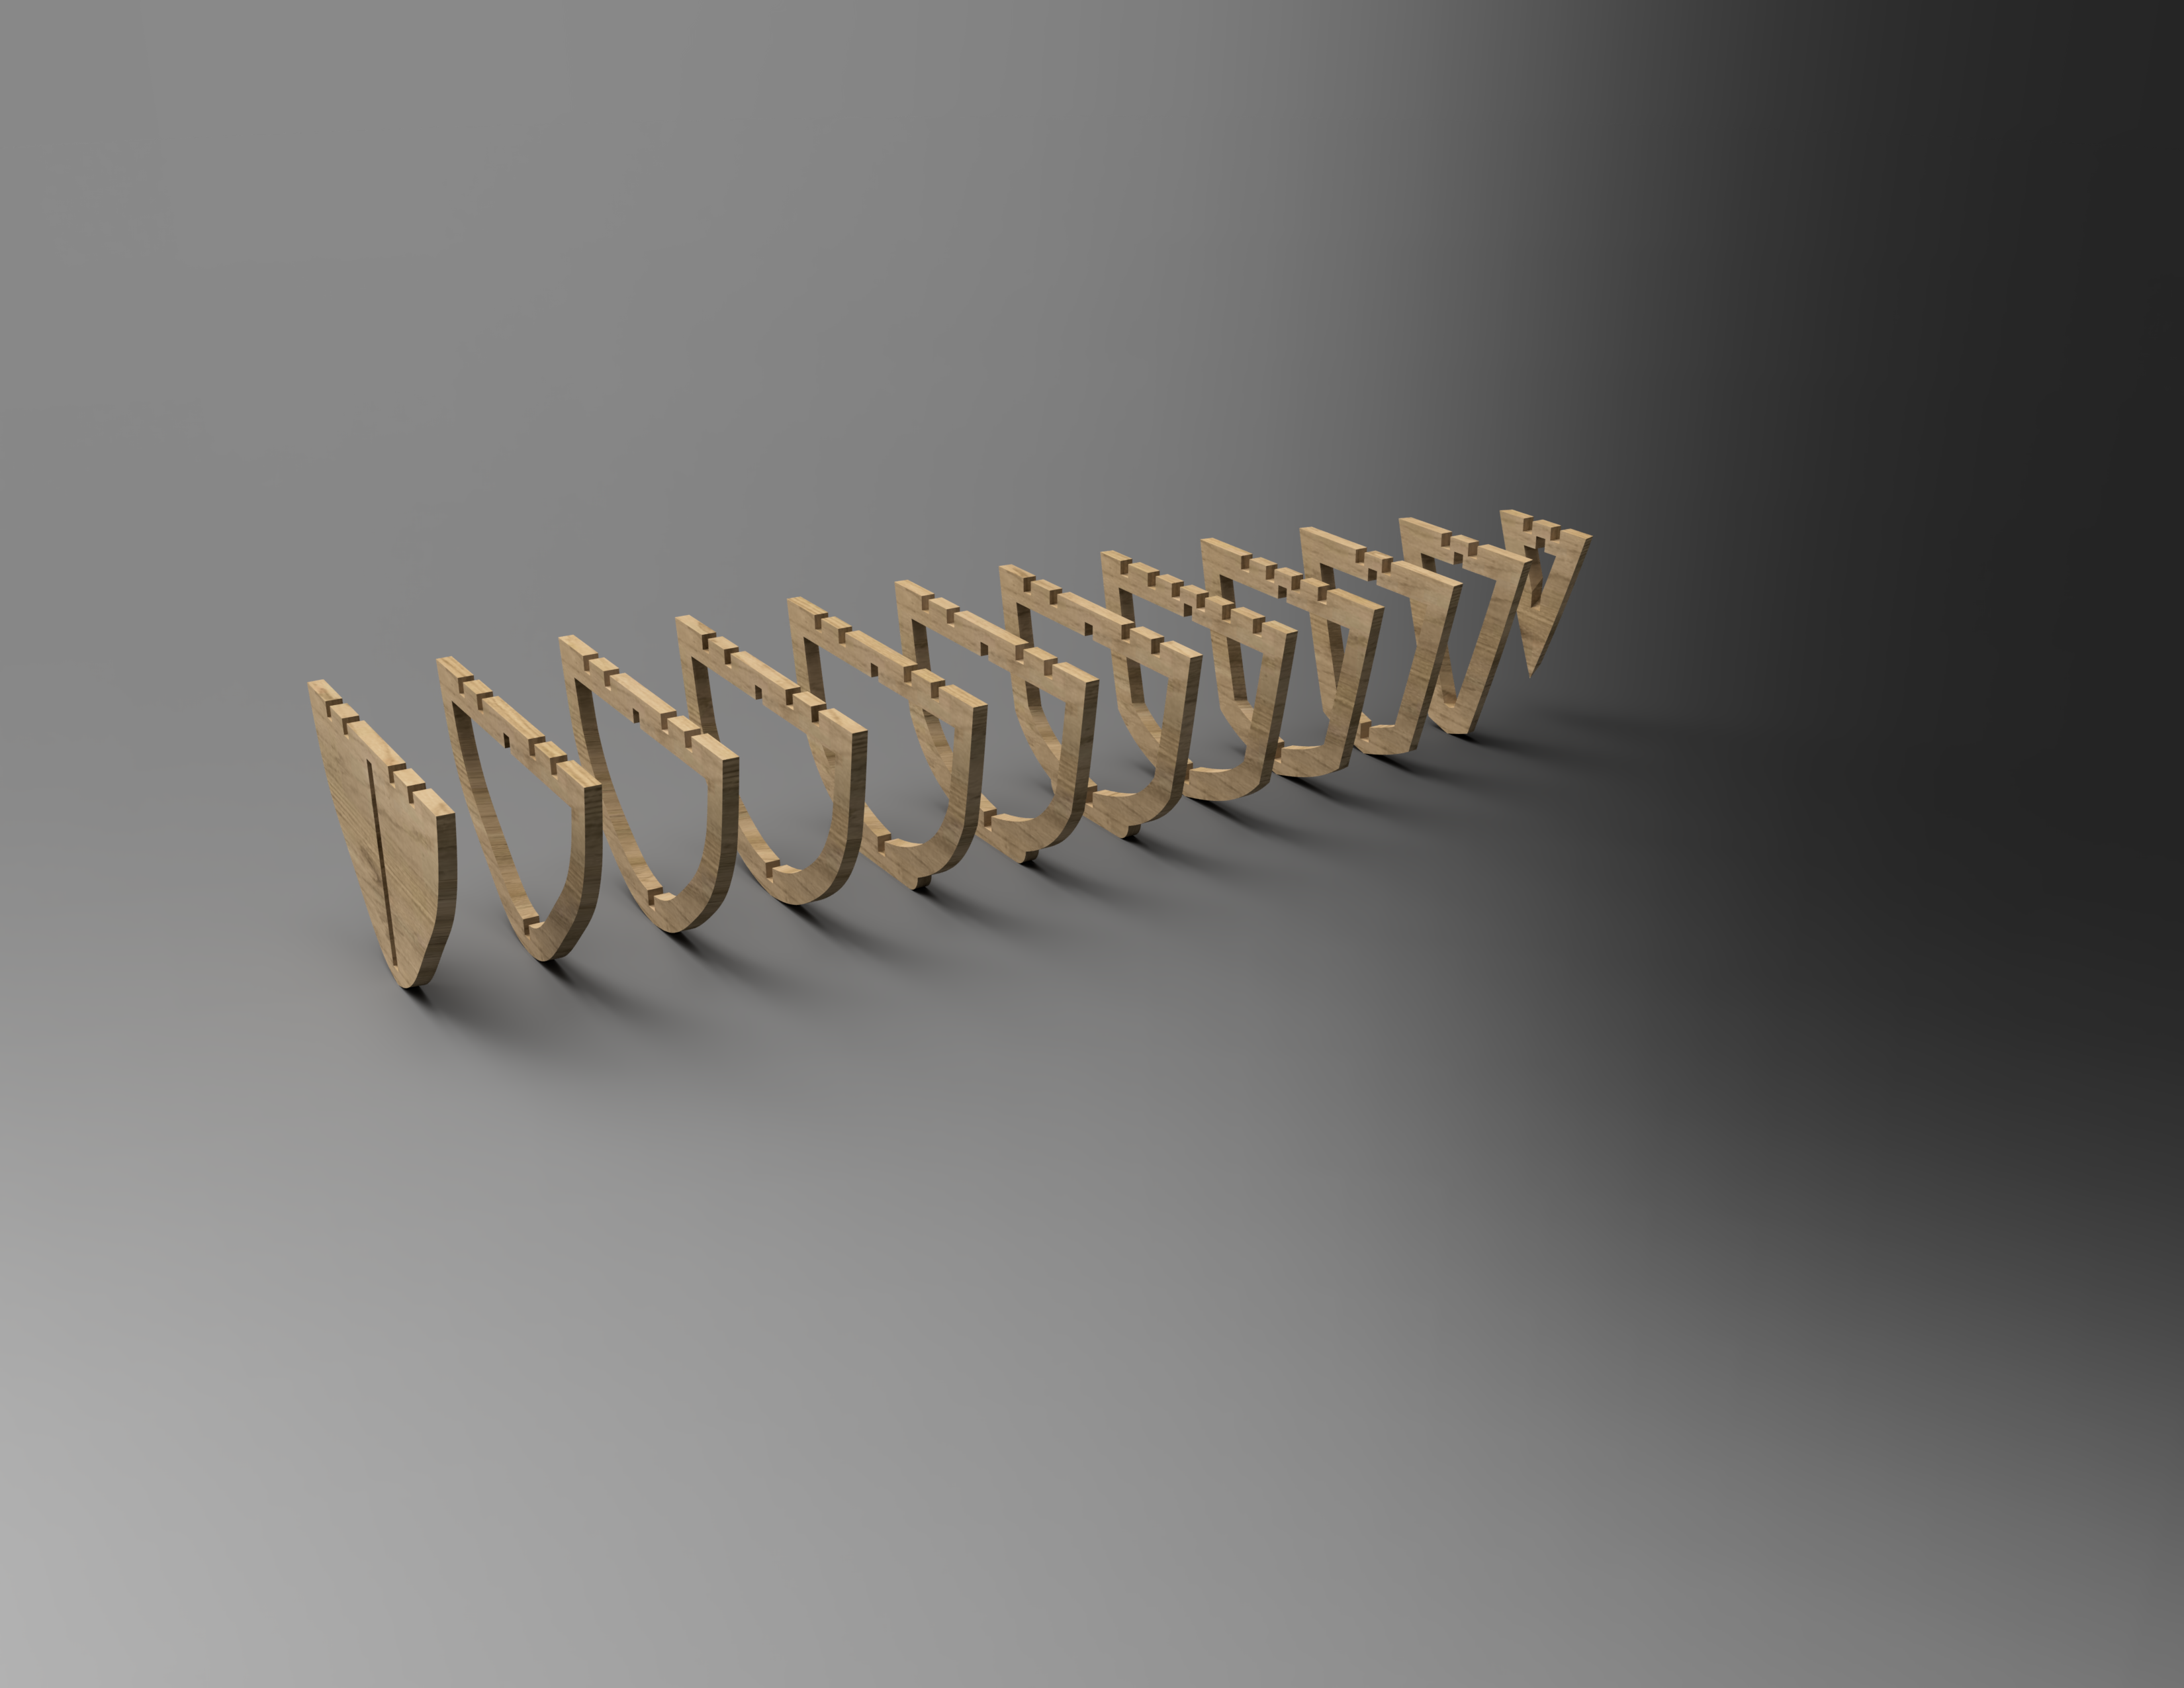
\includegraphics[width=\textwidth]{assets/rippenv1.png}
%  \caption{Render einer ersten Version des Rippenmusters (nicht Final) }
%  \label{fig:rippenv1}
%\end{figure}



\section{Segel und Sailflap}
Die Grundlegende Form des Segels wurde von Tretow  übernommen, aus seiner breiets erwähnten Arbeit "Design of a free-rotating wing sail for an autonomous sailboat" \cite{Tretow2017DesignOA}
Übernommen wurde jedoch lediglich die Aerodynamische Grundform und nicht der gesamte Segelaufbau.

\begin{figure}[H]
    \centering
    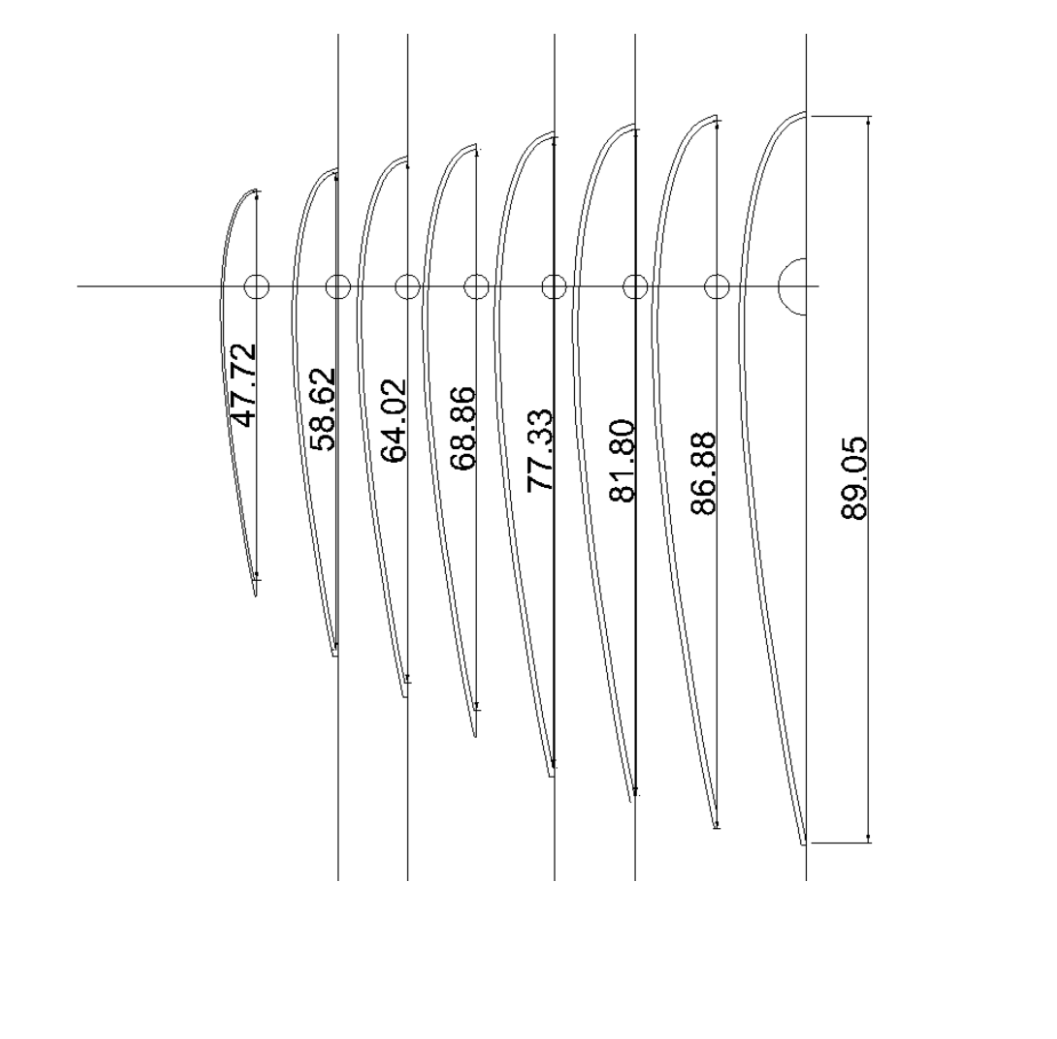
\includegraphics[angle=270,width=0.5\linewidth]{assets/sail_form_foam.png}
    \caption{Segelform von Tretwo aus Design of a free-rotating wing sail for an autonomous sailboat}
    \label{fig:enter-label}
\end{figure}

Das Segel welches in dieser Arbeit behandelt wird, behaltet seine Grösse und wird nicht kleiner um den Herstellungsprozess zu vereinfachen. Dies bringt auch Nachteile, vor allem, da durch die Hebelkraft, der Obere Teil des Segels deutlich mehr Drehmoment auf das Boot bringt, was zu einer stärkeren Schräglage führen könnte. Da die Segelfläche jedoch eher gering ist, wird dies als kein grosses Problem erwartet.

\section{Entwicklungsprozess des Kiels}

Bei der  Konstruktion des Bootes wird auf eine klasssische Kielkonstruktion verzichtet, dieses aus Stabilitätsgründen aber zwingend mit einem Balastkiel ausgestatet werden muss, kann dieser nicht wie üblich an der an der Der Kiel hat die Form eines Kurzkiels. Er  wird aus  5  Teilen zusammengesetzt. 


Die meisten Boote und Schiffe verfügen über einen mittschiffs im Boden angebrachten Längsverband, der das Rückgrad des Bootes bildet


Oben wird bei der Beschreibung der Konstruktion des Bootskörpers ausgeführt, dass von der klassischen Bauweise mit einem über die gesamte Länge des Bootes reichenden Kiel abgewichen wird.\\
Der Kiel dient bei Booten aber nicht als Rückgrad der Rumpfkonstruktion, sondern vor allem auch der Stabilisierung des Bootes im Wasser, der Erhöhung der Kursstabilität, sowie, gerade bei Segelbooten sehr wichtig, der Verringerung der seitlichen Abdrift. \\






\chapter{Elektronik}
Für die Elektronik ist Iterativ implementiert.
Anfangs wird mit einzelnen "Break out boards" gearbeitet. Diese sind einfach zu verbinden und können so relativ schnell zu einer funktionierenden Implementierung führen.

Diese haben jedoch das Risiko, dass das die Schaltungen sehr unübersichtlich werden. Daher wird im verlauf des Projektes eine Platine entwickelt. Das Kapitel zur ersten Implementierung ist im Anhang zu finden. Im weiteren wird die finale Bordelektronik beschrieben mit jeweiligen Anmerkungen und Verbesserungen.


\section{Grundanforderungen an die Elektronik}
Das Segelboot sollte über die nötigen mittel verfügen, eigenständig einen Kurs zu berechnen. Dafür wird ein Mikrocontroller benötigt.
Dieser muss mit Strom versorgt werden. Daher ist auch ein Energiesquelle notwendig. Um Autonomie zu gewährleisten muss diese durchgehend sein. Daher wird ein Energiepuffer bzw. eine Batterie benötigt. Der Gesamtenergieverbrauch des Bootes sollte im schnitt nicht mehr 0.8 W betragen. 

Damit der Mikrocontroller einen Kurs berechnen kann, müssen Umweltdaten bekannt sein. Diese sollen über Sensoren gemessen werden. Um den Kurs auch anzuwenden muss mit der Umwelt interagiert werden. Dafür sind Aktuatoren vorgesehen.






 \subsection{Grundaufbau der Platine}
Um eine übersichtliche Implementierung der Bordelektronik zu gewährleisten wurde eine Platine entwickelt.


\begin{figure}[H]
    \centering
    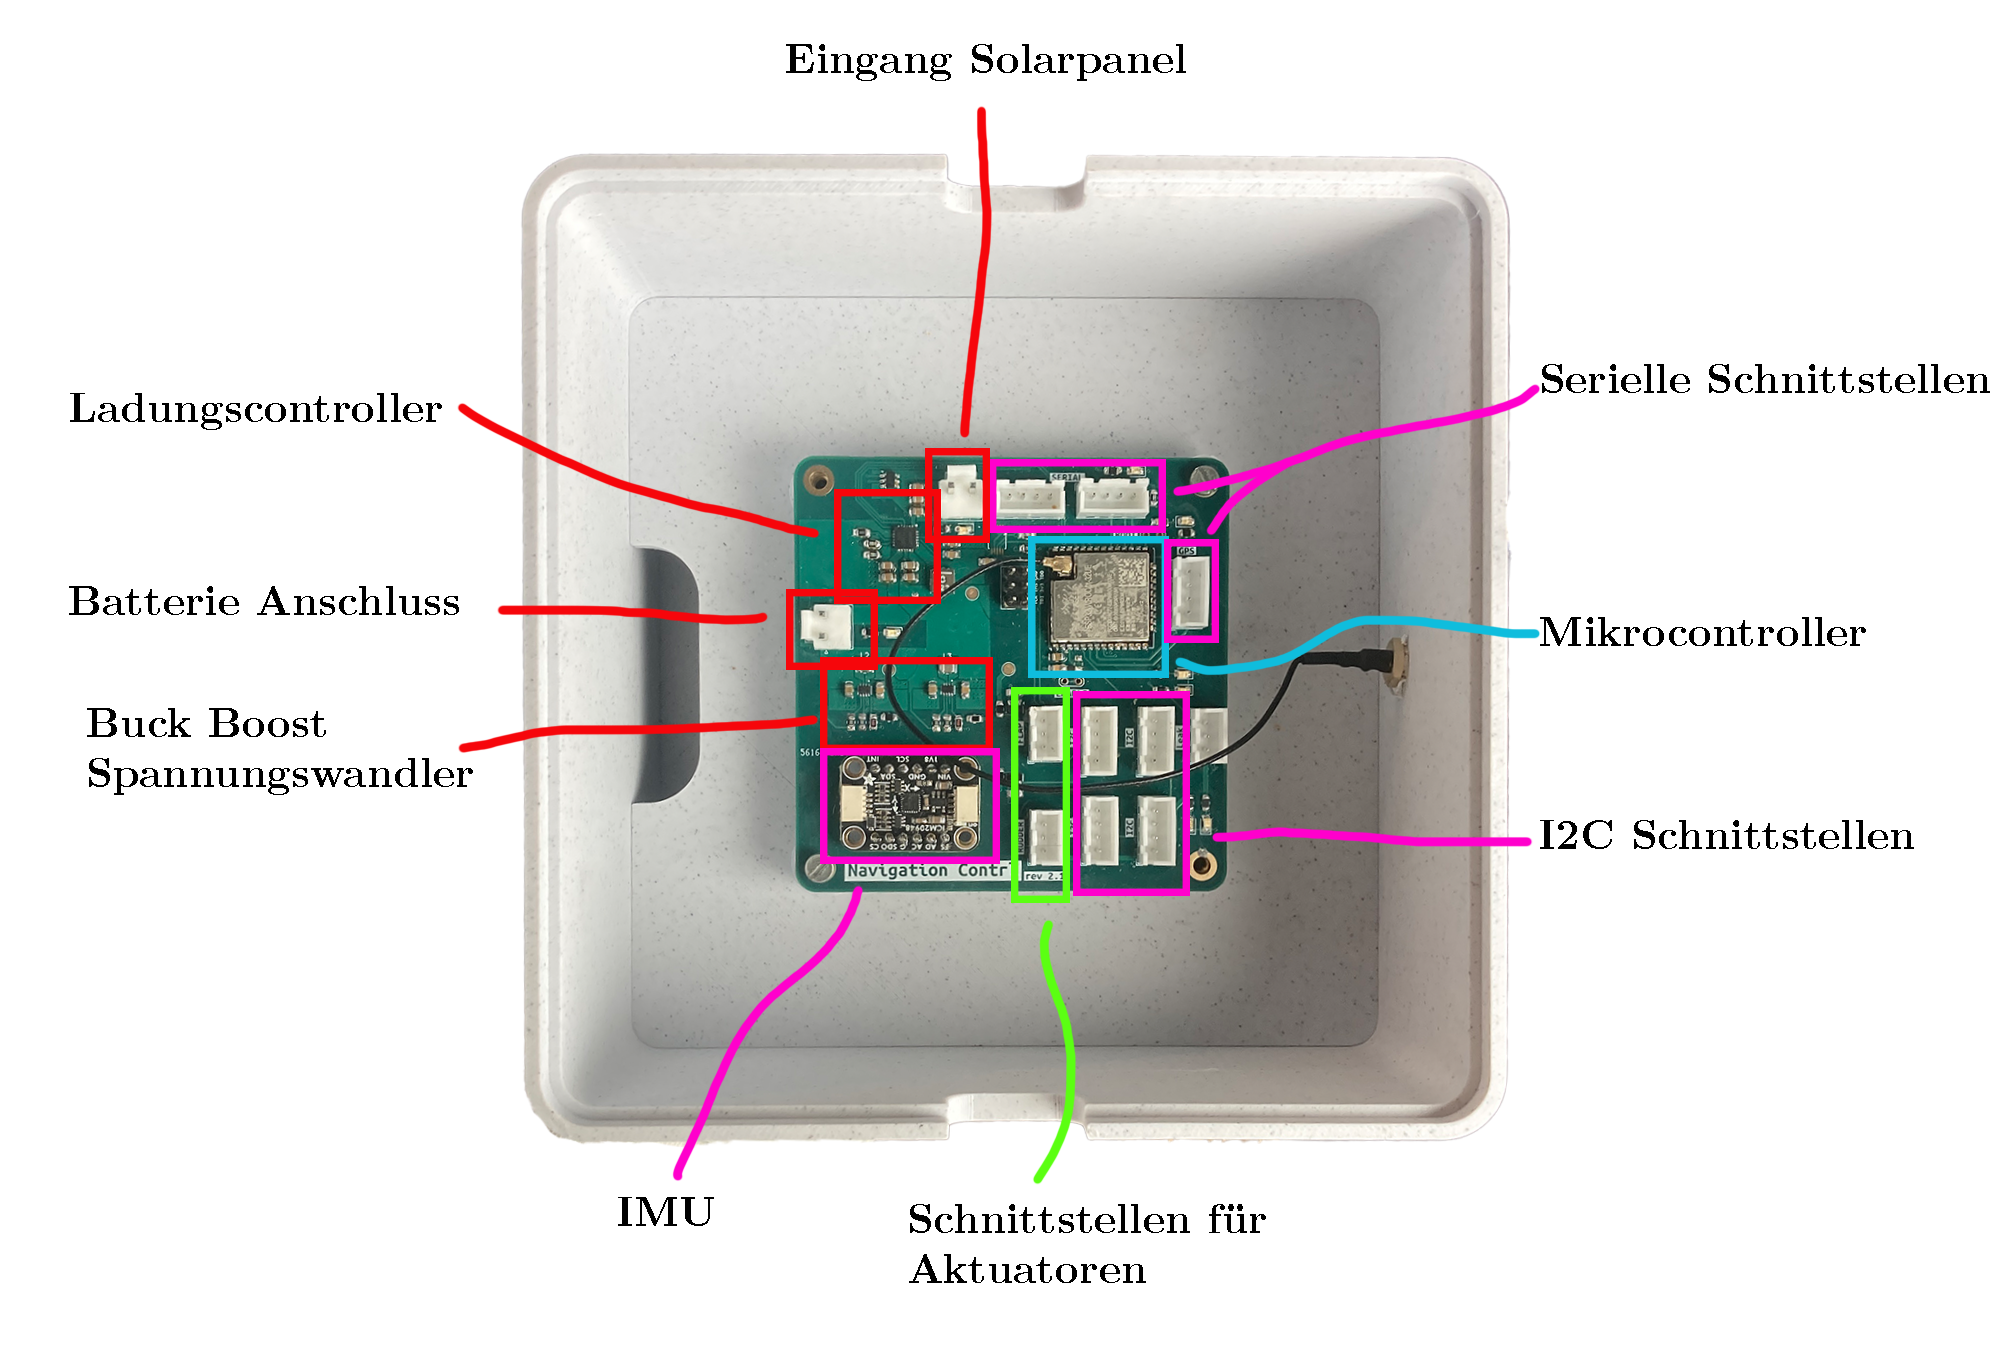
\includegraphics[width=1\linewidth]{Overview PCB_colored.png}
    \caption{Grundkomponenten der Platine}
    \label{fig:core_pcb}
\end{figure}
 
\begin{figure}[H]
    \centering
     \begin{subfigure}[b]{0.38\linewidth}
        \centering
        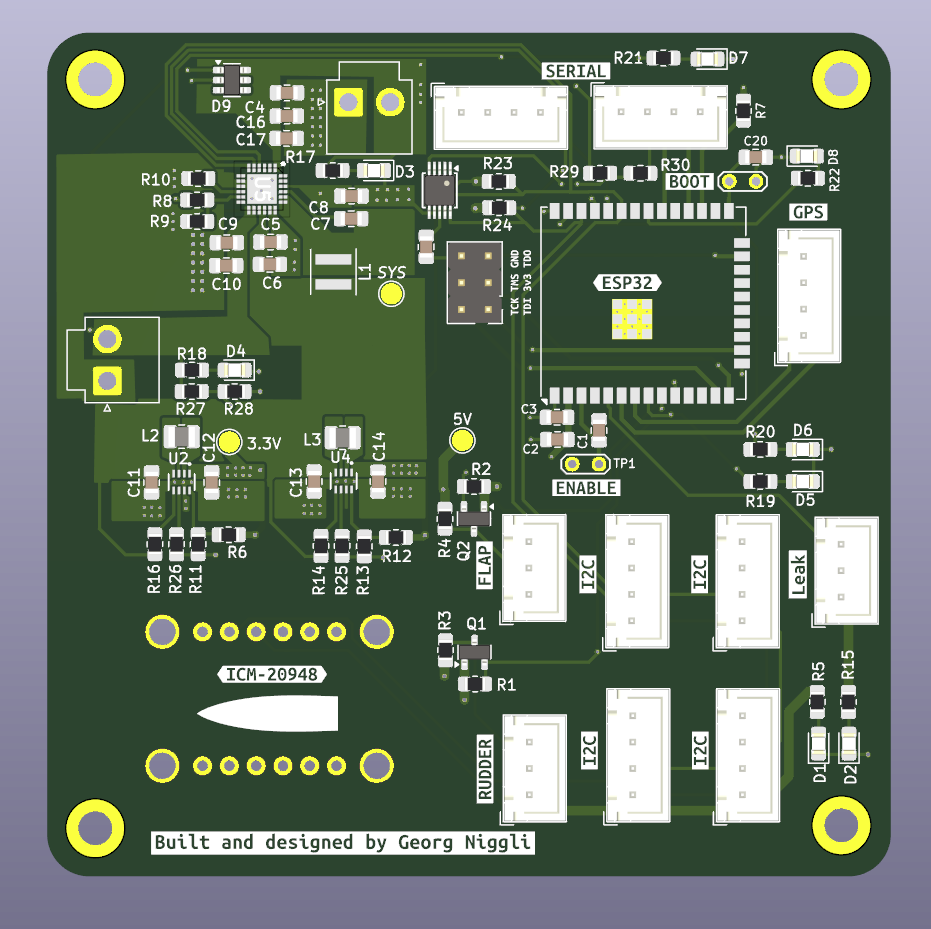
\includegraphics[width=\linewidth]{assets/pcb_2.png}
        \caption{Platine – Ansicht 3D}
        \label{fig:pcb_2}
    \end{subfigure}
    \hfill
      \begin{subfigure}[b]{0.38\linewidth}
        \centering
        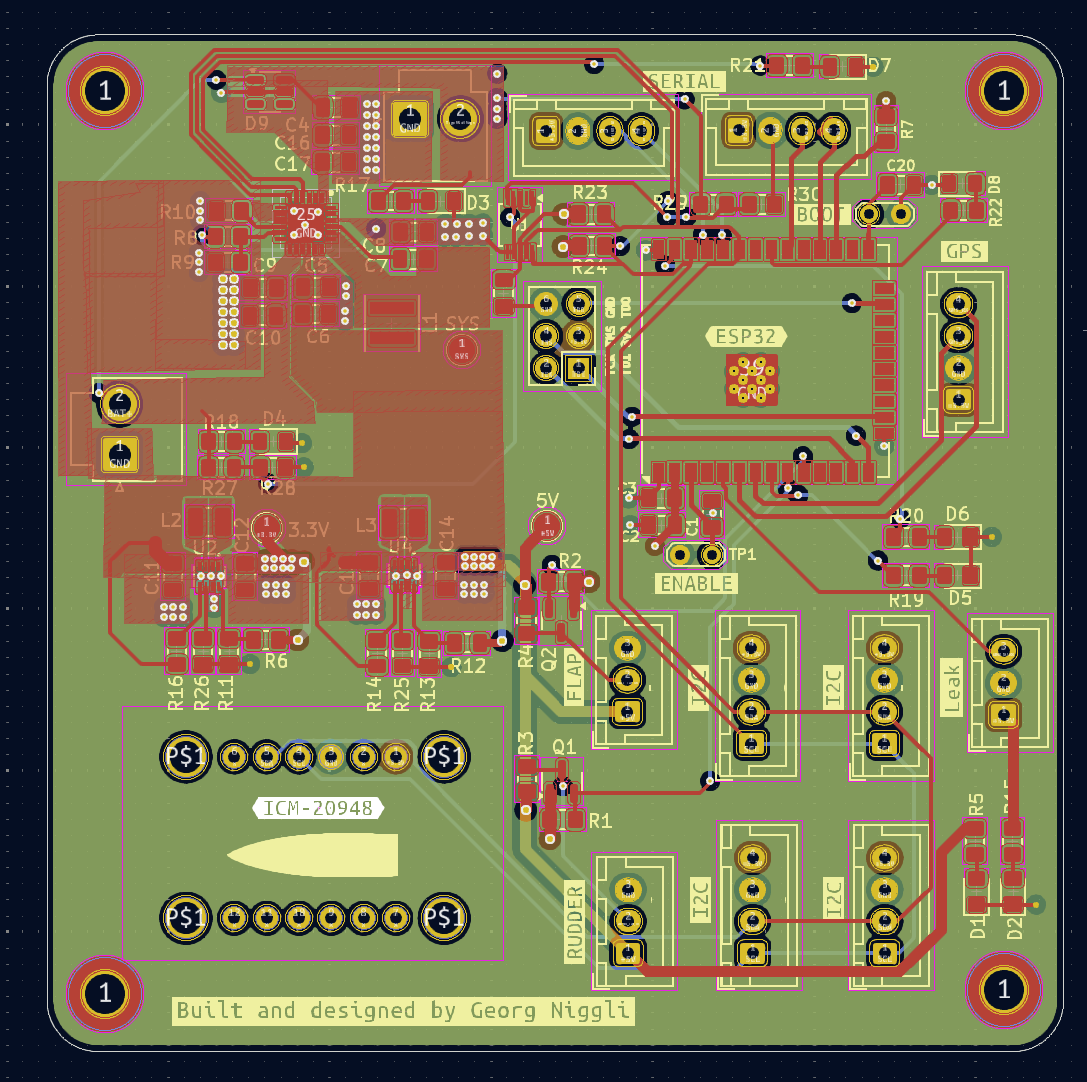
\includegraphics[width=\linewidth]{assets/pcb_1.png}
        \caption{Platine – Ansicht KiCad}
        \label{fig:pcb_1}
    \end{subfigure}
    \caption{Zwei Ansichten der entwickelten Leiterplatte}
    \label{fig:pcb_views}
\end{figure}


Die Grundkomponenten lassen sich wie in Abbildung \ref{fig:core_pcb} farblich dargestellt, in vier Kategorien aufteilen.
\begin{itemize}
    \item Mikrocontroller: Blau
    \item Energie und Leistungselektronik: Rot 
    \item Sensoren: Pink
    \item Aktuatoren: Grün 
\end{itemize}


\subsection{Mikrocontroller}

Ein ESP32-WROOM-32UE-N8R2 Modul von Espressif wird als Mikrocontroller verwendet. Module dieser Form werden aus einer zusätzlichen Platine hergestellt die alle essenziellen Funktionsschaltungen integriert haben. Somit könnend diese einfacher in neue Schaltungen integriert werden.\ref{ESP32Datasheet}

ESP32 Mikrocontroller sind sehr beliebt für ihre einfache Programmierung in der Arduino Umgebung. Zudem sind die Drahltloskommunikationsprotokolle WLAN und Bluetooth Low Energy (BLE) von Haus aus eingebaut. Im folgenden wird BLE verwendet.

Gewählt wird dieser Mikrocontroller aufgrund seiner relativ einfachen Programmierung im Vergleich zu anderen eingebetteten Systemen. Seine Rechenleistung reicht für die gewählte Implementierung des Navigationsalgorithmus aus. Der ESP32 ist nicht der Energiesparendste Mikrocontroller. Mit einem Energieverbrauch von 130 mA beim kommunizieren über Bluetooth Low Energy (BLE) liegt dies mit 0.4W noch deutlich unter der angepeilten Wattstunde und läst noch viel Raum übrig für die restlichen Bauteile.

Ein Raspberry Pi, der in der vorherigen Iteration verwendet wird, hat sich in der Implementierung als schwieriger dargestellt. Die Interaktion mit Sensoren über den eigentlich unterstützten I2C Bus hat nicht immer zuverlässig Funktioniert. Da die zusätzlichen Funktionen die eine Linux Umgebung bieten nicht benötigt werden, wird die einfachere und zuverlässigere Alternative gewählt.


\subsection{Batterieladung}
Zur geregelten Ladung des Akkumulators wird ein 5-A-Modul mit dem Lade-IC BQ25895 von Texas Instruments eingesetzt.  
Lithium-Ionen-Akkumulatoren dürfen nicht ausschliesslich mit konstantem Strom geladen werden. In Abbildung~\ref{fig:battery-curve} ist ein Diagramm aus dem Datenblatt des Lade-ICs dargestellt, das den typischen Verlauf eines Ladevorgangs zeigt. Dieses Ladeverfahren gewährleistet einen sicheren und Akkuschonenden Betrieb.

\subsubsection{Ladeprozess von Li-Ionen-Akkumulatoren}

\begin{figure}[H]
    \centering
    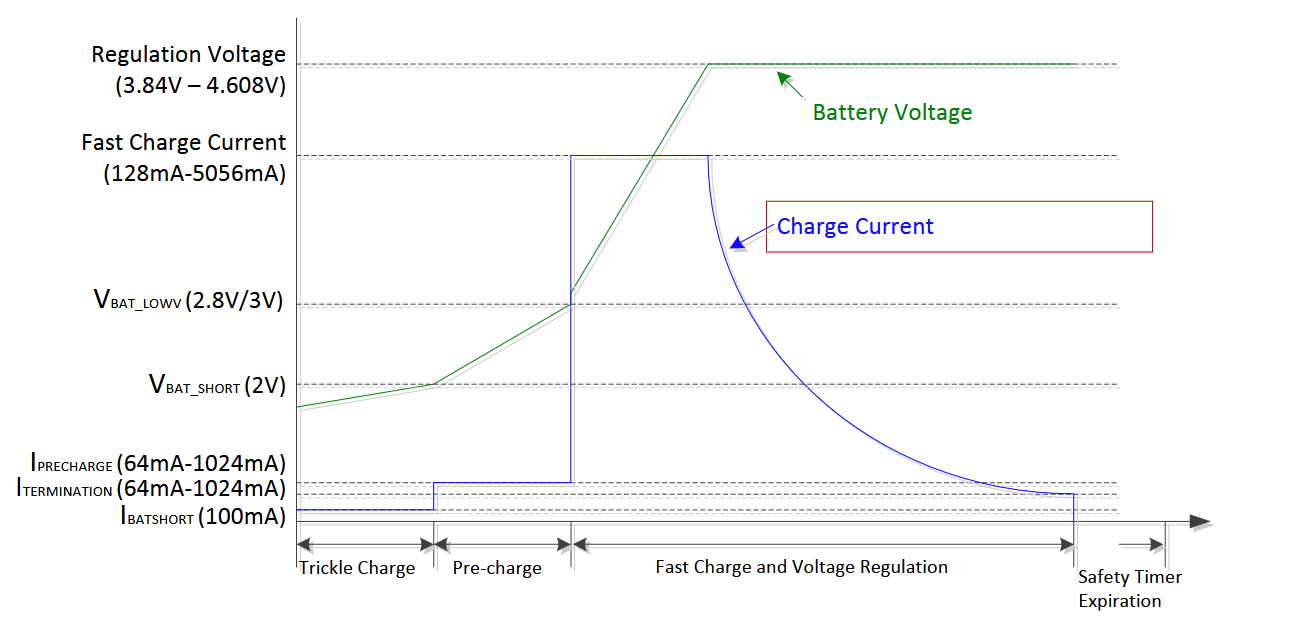
\includegraphics[width=0.7\linewidth]{batteryChargeCurve.png}
    \caption{Batterie Lade Kurve}
    \label{fig:battery-curve}
\end{figure}

Der Ladevorgang eines Lithium-Ionen-Akkumulators erfolgt in zwei Hauptphasen gemäss dem \textbf{CC-CV-Verfahren} (Constant Current – Constant Voltage):

\begin{itemize}
    \item \textbf{Konstantstromphase (CC):}  
    Zu Beginn des Ladevorgangs wird der Akku mit einem konstanten Strom geladen. Dabei steigt die Zellenspannung kontinuierlich an, bis sie den maximal zulässigen Wert erreicht (typischerweise 4{,}2\,V pro Zelle). Diese Phase dient dem schnellen Auffüllen der Zellkapazität und dauert etwa 60--70\,\% der gesamten Ladezeit.

    \item \textbf{Konstantspannungsphase (CV):}  
    Nach Erreichen der maximalen Zellspannung wird die Spannung konstant gehalten, während der Strom allmählich abnimmt. In dieser Phase erfolgt die vollständige Sättigung der Zelle mit Ladungsträgern.
\end{itemize}

Der Lade-IC BQ25895 erkennt das Ladeende automatisch anhand des sogenannten Terminationsstroms (\textit{I\_TERM}). Sobald der Ladestrom in der Konstantspannungsphase unter diesen Schwellwert fällt, beendet der IC den aktiven Ladevorgang. Der Terminationsstrom ist über das Register \texttt{CHARGE\_TERMINATION\_CURRENT} (Adresse \texttt{0x05}) konfigurierbar und beträgt standardmssig \textbf{180\,mA} 

Nach Erreichen dieses Punktes wechselt der IC in den Standby-Modus. Sollte die Zellenspannung später unter einen definierten Schwellenwert (typisch ca. 4{,}1\,V) fallen, wird der Ladevorgang automatisch erneut gestartet. Diese automatische Ladeende-Erkennung schützt den Akku vor Überladung.

Durch die Kombination der beiden Ladephasen sowie der intelligenten Ladeüberwachung wird eine sichere, vollständige und akkuschonende Ladung erreicht.


\subsection{Aufbau der Batterie}
Es ist vorgesehen, dass die Energiereserve einen Betrieb während zwei Tagen (48 h) erlauben soll. Der genaue Energieverbrauch des Rechners, der Sensoren und vor allem der Aktuatoren hängt stark davon ab, wie oft Steuereingriffe vorgenommen werden müssen und Messdatenerfassungen Neuberechnungen erfolgen. Es lässt sich daher nicht präzis berechnen, sondern nur abschätzen. 

Der Richtwert für den Gesamtenergieverbrauch pro Stunde beträgt maximal 0.8 Watt. Das ergibt einen Energieverbrauch von 19.2 Wattstunden pro Tag (24 h). Zur Überbrückung der vorgesehenen zwei Tagen ohne Energiezufuhr muss der Speicher daher über eine Kapazität von 38.4 Wattstunden verfügen. 

Eine völlige Erschöpfung des Energiespeichers kann diesen schädigen. Sie muss daher verhindert werden. Aber bereits ein Absinken der Ladung auf unter 20 Prozent verkürzt dessen Lebensdauer. Die Kapazität muss daher erhöht werden. Um über Reserven zu verfügen, wird daher eine Kapazität von 46.25 Wattstunden vorgesehen.

Für den Energiespeicher sollen 5 günstige wiederaufladbare EVE ICR18650 Litium-Ionen Zellen der chinesischen EVE Energy CO., LTD verwendet werden. Die Zellen haben eine Kapazität von 2'550 mAh un eine für Li-Ion übliche Nennspannung von 3.7 V.

\begin{figure}[H]
    \centering
    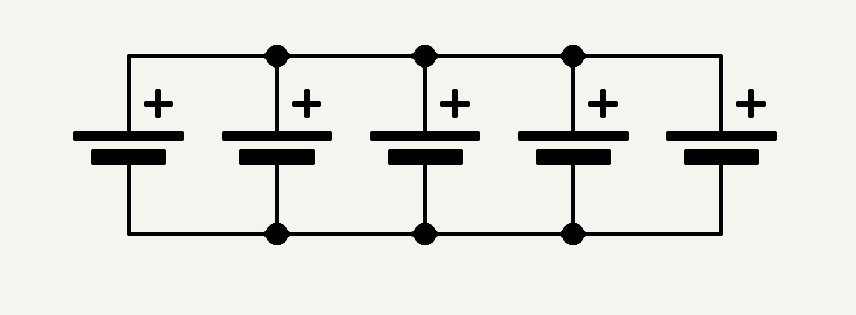
\includegraphics[width=0.5\linewidth]{assets/batterie_5p.png}
    \caption{Batterie 5 Parallel}
    \label{fig:bat5p}
\end{figure}

Es werden 5 Zellen parallel zusammengeschweisst. Hierfür wird ein übliches verfahren aus der Batterieherstellung verwendet. Das Punktschweissen. Es wäre an sich möglich, die Nikkelbänder mit denen die Zellen verbunden sind, zu verlöten. Dabei besteht aber die ernste Gefahr, dass die Zellen mit dem Lötkolben zu lange und zu stark erhitzt werden. Sie können dabei nicht nur unrettbar beschädigt werden, sondern sich auch entzünden.


Der Ladecontroller verfügt zudem über PowerPath was für die Anwendung in Autonomen Gefährten essenziell ist. PowerPath beschribt den Vorgang, bei dem das System durchgehend mit Enegerie versorgt wird. Auch dann, wenn die Batterie geladen wird. Somit kommt es zu keinen Unterbrüchen welche in dieser Anwendung verehrende Folgen haben könnten. 


\subsection{Energieversorgung}

Rechner, Sensoren und Aktuatoren werden mit elektrischer Energie betrieben. Weil das Segelboot autonom funktionieren soll, muss diese auf dem Schiff selbst gewonnen werden. Infrage kommen dabei grundsätzlich drei Energiequellen, nämlich Wasserenergie, Windenergie und Sonnenenergie.

\subsubsection{Wasserturbine}
Da sich das Boot im Wasser bewegt, könnte eine kleine Wasserturbine am Bootskörper befestigt und die Strömung zu deren Antrieb genutzt werden. Da sich das Boot relativ zum Wasser bewegt, gelten die gleichen Prinzipien wie bei Generierung elektrischer Energie durch Wasserkraft in Fliessgewässern.

Diese Methode hat jedoch gewichtige Nachteile. Segelboote erreichen, abgesehen von speziellen Konstruktionen wie sog. Foilingboote, bei denen der Bootskörper bei Fahrt vollständig aus dem Wasser gehoben wird, nur bescheidene Geschwindigkeiten. Da die Leistung einer Turbine in einer Flüssigkeit bei gleicher Fläche kubisch zur Strömungsgeschwindigkeit ansteigt, erlaubt diese Methode selbst bei idealen Segelbedingungen nur eine geringe Energieausbeute. Zudem würde das Segelboot durch die Turbine empfindlich abgebremst. 

\subsubsection{Windturbine}
Auch die Generierung von elektrischer Energie mithilfe einer Windturbine unter Nutzung der Windkraft ist nicht praktikabel. Um die Windenergie in Bewegungsenergie umzusetzen, aus der dann elektrische Energie generiert werden kann, muss ein Windrad in den Wind gedreht werden. Ein Segelboot kann keinen Kurs gegen den Wind segeln. Der Kurs vor dem Wind (also ein Kurs, bei dem der Wind von hinten auf das Boot trifft) ist zwar möglich, aber wenig effizient. Ein Windrad könnte folglich nicht fix mit dem Boot verbunden werden, sondern müsste drehbar ausgelegt werden, damit es unabhängig vom Kurs des Bootes in den Wind gedreht werden kann. Es müsste so platziert werden, dass nicht nur eine Berührung des Segels, sondern auch eine Berührung der Wasseroberfläche bei einer Kränkung (Schieflage) des Bootes ausgeschlossen ist. Damit müsste es am äussersten Bug, am äussersten Heck oder auf dem Mast platziert werden. Alle Positionen verbieten sich, da damit die Balance des Bootes akut gefährdet wäre. 

Schliesslich würde eine Positionierung am Bug oder Heck je nach vorherrschendem Wind, zu einer vollen oder teilweisen Abschattung des Windrades durch das Segel oder des Segels durch das Windrad führen. Eine Positionierung auf dem Mast würde selbst im Fall eines Vertikalwindrades zu Verwirbelungen führen, welche die Segeleigenschaften des Bootes negativ beeinträchtigen würden.

\subsubsection{Fotovoltaik}
Für die Nutzung der Sonnenenergie auf dem autonomen Segelboot kommt nur die Methode der Fotovoltaik infrage. Die für den Betrieb von Wärme-Kraft-Maschinen erforderlichen Temperaturen lassen sich auf einem beweglichen Boot mit Sonnenenergie nicht erreichen.

Die Energieerzeugung mit Fotovoltaikanlagen ist auf Segelbooten beliebt und verbreitet. Solche Anlagen haben keinen Einfluss auf die Segeleigenschaften des Bootes. Die Energieausbeute hängt aber stark vom Sonnenstand und dem vorherrschenden Wetter ab. Im Gegensatz zu stationären Anlagen lassen sich Fotovoltaikanlagen auf Booten nicht ideal auf die Sonne ausrichten und können je nach Kurs sogar vom Segel beschattet werden. Da während der Nachtstunden überhaupt keine Energie gewonnen werden kann, muss das Boot zur Überbrückung zwingend mit einem Energiespeicher ausgerüstet werden.

Das Solarpanel kann auf dem Deck oder am Festsegel befestigt werden. Die Befestigung auf dem Deck hat den Vorteil, dass die Verbindungsleitung zum Energiespeicher nicht durch den Schleifring geführt werden muss. Sodann ist die sichere Befestigung am flachen Deck einfacher als am gewölbten Festsegel. Schliesslich müssten bei einer Montage am Segel zwei Panels verwendet werden, damit beide Seiten des Festsegels damit ausgerüstet werden können. Andernfalls bestünde die Gefahr, dass sich das Panel bei einem ungünstigen Kurs längere Zeit auf der Schattenseite des Festsegels befindet.  

Der Selbstbau eines Panels wird nach einer längeren Erkundungsphase verworfen, da komplette, für den mobilen Einsatz entwickelte Panels kostengünstiger sind.   

Es wird das portable und faltbare Pi Juice Solar Panel - 22 Watt der britischen Pi Supply (Nebra Ltd) verwendet. Es ist gegen Spritzwasser geschützt (IP4X-Kennzeichnung), misst im entfalteten Zustand 83x23 cm und wiegt 520 g. Die vier einzelnen Panels sind von einer Textilhülle umfasst, die vier Befestigungsösen aufweist. Mit diesen wird das Panel vor dem Mast auf der flachen Deckplatte des Segelboots befestigt.

Bei den Solarzellen handelt es sich um monokristalline Siliziumzellen. Diese zeichnen sich durch einen hohen Wirkungsgrad sowie eine lange Lebensdauer aus und sind aufgrund ihrer gleichmässigen Kristallstruktur besonders effizient bei direkter Sonneneinstrahlung.

Ein wesentliches Problem bei der Verwendung von Solarzellen ist die Teilverschattung. Unter Teilverschattung versteht man die teilweise Abschattung einzelner Zellen oder Zellbereiche innerhalb eines Solarmoduls.

Das elektrische Verhalten von Solarzellen unter Teilverschattung ist nicht linear. Da Solarzellen innerhalb eines Moduls meist in Reihe geschaltet sind, bestimmt die am stärksten verschattete Zelle den Stromfluss im gesamten Strang. Wird eine einzelne Zelle teilweise verschattet, so sinkt deren Stromproduktion lokal erheblich. Aufgrund der Reihenschaltung wirkt die verschattete Zelle wie ein elektrischer Widerstand oder sogar als Last, was zu einem Leistungsabfall im gesamten Modul führen kann.

Da die Energieausbäute  des Solapanels jedoch genug sein sollte, kann auf Phasen mit weniger Ausbäute verzichtet werden.

Ebenfalls nicht implementiert ist ein Maximum Power Point Tracking (MPPT) jedoch verfügt der Batterieladungscontroller über Input Current Optimizer (ICO)

\textbf{Unterschied zwischen ICO und MPPT:}
Der ICO und das MPPT sind zwei unterschiedliche Verfahren zur Leistungsoptimierung bei Energiequellen wie Solarpanels. Während MPPT darauf abzielt, den Arbeitspunkt des Panels so zu regeln, dass die abgegebene Leistung (Produkt aus Spannung und Strom) maximal ist, konzentriert sich ICO auf die Optimierung des Eingangsstroms. MPPT ist komplexer, reagiert dynamisch auf Umweltbedingungen und wird meist in grösseren Solaranlagen eingesetzt. ICO hingegen wird typischerweise in integrierten Power-Management-ICs verwendet, wie dem verwendeten BQ25895, und bietet eine einfachere Möglichkeit, die Quelle vor Überlastung zu schützen, indem es den optimalen Eingangsstrom einstellt.


Die maximale regulierte Ausgangsleistung beträgt 20 W bei 5 V. Es verfügt über zwei 5 V/ 2.4 A USB Ausgänge, wobei die maximale Ausgangsleistung pro USB Buchse auf 12 W beschränkt ist. Die zwei USB Buchsen können simultan benutzt werden.
\begin{figure}[H]
\centering
    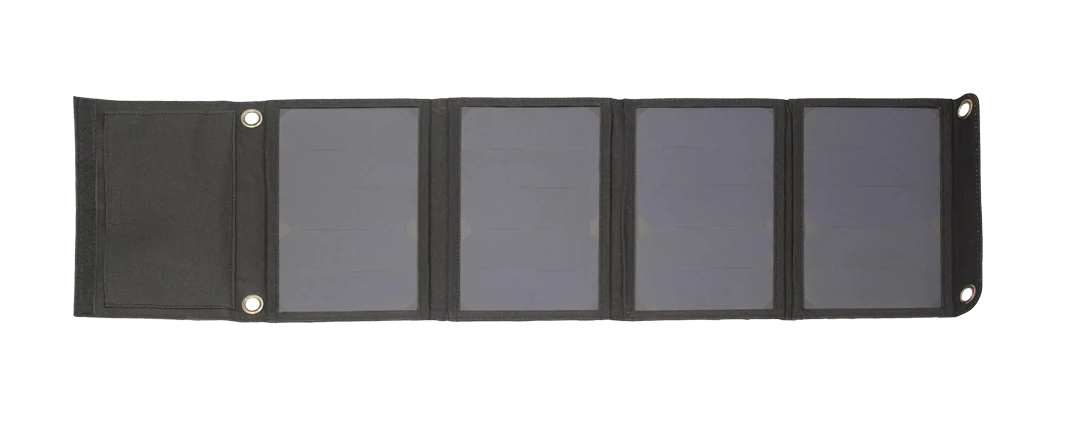
\includegraphics[width=1\linewidth]{assets/Pi juce.png}
    \caption{Pi Juce Solarpanel}
    \label{fig:enter-label}
\end{figure}

\subsection{Leistungselektronik}
Da sich auf dem Boot verschiedene Spannungen befinden, sind Spannungswandler notwendig. Der Mikrocontroller und alle Sensoren benötigen 3.3 V. Die Aktuatoren zur Steuerung des Ruders und des Segels benötigen 5V. Das Solarpanel hat eine Spannung von 5V und die Batterie eine Nennspannung von 3.7. Dieser Wert kann jedoch zwischen 3.3 V und 4.2 V variieren. Abhängig von der Ladung der Batterie.

Um nun geregelte Spannungen zu erzeugen werden zwei Buck Boost Konverter verwendet. 

Ein Buck-Boost-Konverter ist eine Gleichspannungswandler-Schaltung, die eine Eingangsspannung \( V_{\text{in}} \) in eine Ausgangsspannung \( V_{\text{out}} \) umwandelt, die entweder grösser oder kleiner als die Eingangsspannung sein kann. 

Der Buck Boost wurde hier im Gegensatz zum Regulären Buck Konverter gewählt, da die Batteriespannung sehr nahe oder sogar unterhalb von den benötigten 3.3 V liegen kann. Es ist essenziell, das dass System auch dann weiter funktioniert.

Verwendet werden zwei TPS631000DRLR vom Unternehmen Texas Instruments. Beide haben eine Effizienz von $\approx$ 90\%.

Die Schaltung ist der "Typical Application" aus dem Datenblatt nachempfunden.
\section{Sensoren und Aktuatoren}
\subsubsection{Positionsbestimmung (GPS)}
Zur Positionsbestimmung, also der Bestimmung des aktuellen Standorts des Segelboots, werden Funksignale des bekannten US-amerikanischen satellitenbasierten Global Positioning Systems (GPS) (deutsch Globales Positionsbestimmungssystem) offiziell NAVSTAR GPS verwendet. Dafür wird das Empfängermodul Whadda Neo 7M der belgischen Velleman Group nv verwendet, welches alternativ Signale des entsprechenden russischen Systems GLONASS empfangen kann.
Das Modul wird wie allen anderen sensoren über JST Stecker mit dem PCB verdrahtet und kommuniziert über eine serielle Verbindung. Das Modul wird mit 3.3 V betrieben.
\begin{figure}[H]
    \centering
    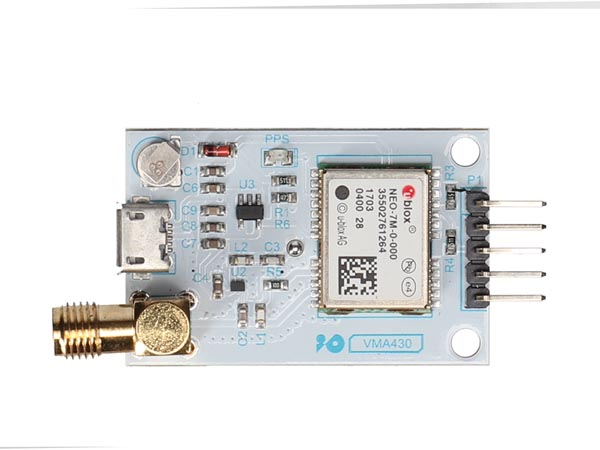
\includegraphics[width=0.75\linewidth]{vma430_front-1.jpg}
    \caption{GPS Modul - Oberseite}
    \label{fig:enter-label}
\end{figure}
Das Modul wird auf dem Deck im des Bootes platziert. Weil das Kunststoffgehäuse sehr dünn ist, kann auf eine externe Empfangsantenne verzichtet werden. Die vorhandene SMA Antennen Steckbuchse bleibt damit unbenutzt. Es wird die eingebaute keramische Patchantenne verwendet. In der unten stehenden Abbildung \ref{fig:GPS} ist diese als rosa Fläche mit einem metallenen Knopf auf einem beigen Körper sichtbar.
\begin{figure}[H]
    \centering
    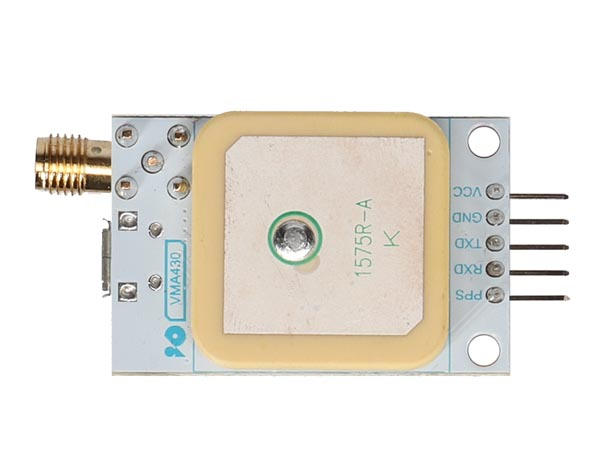
\includegraphics[width=0.5\linewidth]{vma430_back-1.jpg}
    \caption{GPS Modul}
    \label{fig:GPS}
\end{figure}

\subsubsection{Gyro und Magnetometer}

Zur Bestimmung der Richtung des Segelboots dient ein Magnetometer. Ein Magnetometer ist eine sensorische Einrichtung zur Messung magnetischer Flussdichten \cite{noauthor_magnetometer_2023}. Im vorliegenden Projekt wird das Magnetometer dafür eingesetzt, um damit einen Magnetkompass zu realisieren, indem das erdmagnetische Feld dreidimensional erfasst wird, um daraus die Bootsrichtung abzuleiten. Dieses Verfahren wird auch in Smartphones zur Richtungsbestimmung angewendet.

Im vorliegenden Projekt wird dafür das Sensormodul ICM-20948 der Firma Adafruit vorgesehen. Das Modul ist zusätzlich mit einem Gyroskop und einen Beschleunigungsmesser ausgestattet. Auch damit kann die Bewegung des Segelbootes erfasst werden. Ausserdem erlaubt es die Bestimmung der Schräglage des Segelbootes. Im vorliegenden Projekt wird dieser Wert erfasst jedoch nicht ausgewertet.

Das Sensormodul wird mit einer Eingangsspannung von 3.3 V betrieben und über den im PCB verbauten I2C Bus angehängt.



\section{Eigenentwicklung des Windrichtungssensors}
Der Windrichtungssensor muss selbst entwickelt und gebaut werden, da die am Markt angebotenen Windrichtungsmesser entweder zu gross und zu schwer oder unerschwinglich teuer sind.

Windrichtungssensoren lassen sich in zwei unterschiedliche Typen einteilen. Der erste Typ verwendet ein Potenziometer zur Richtungsbestimmung. Solche Messgeräte sind mechanisch sehr leicht umzusetzen, da dazu lediglich ein kleiner Flügel an der Achse eines Potenziometers befestigt werden muss. Die Position des Flügels kann damit über einen analogen Input Pin mit einem Mikrocontroller eingelesen und daraus die Richtung des Windes abgeleitete werden. Der Nachteil dieses Typs ist, dass die freie Drehung der Achse durch die Reibung das Potenziometers stark abgebremst wird. Dieser Typ wird daher nicht weiter verfolgt.

Der andere Typ verwendet Hallsensoren, welche den Hall-Effekt zur Messung von 
Magnetfeldern nutzen \cite{noauthor_hall-sensor_2023}. Sie sind passive Sensoren, die den Spannungsunterschied messen, der an einem elektrischen Leiter erzeugt wird, wenn ein Magnetfeld senkrecht zur Fliessrichtung eines elektrischen Stroms steht \cite{noauthor_alles_nodate}. Um die Rotation eines Objektes mittels Hallsensoren zu messen, gibt es die folgenden zwei Möglichkeiten:

Bei der ersten Variante wird um ein abwechselnd magnetisch positiv und magnetisch negativ geladenes rundes Objekt mehrere Hallsensoren platziert. Damit kann dann die Drehung des Objektes gemessen werden. Diese Variante ist praktisch schwierig umzusetzen, weil viele Hall Sensoren präzis kreisförmig um eine Achse angeordnet werden müssen. Diese Variante ist jedoch sehr umständlich im Vergleich zur zweiten Variante.

Die zweite Variante ist praktisch einfacher umzusetzen. Statt normale Hall Sensoren werden dabei spezielle, sogenannten Rotary Hall (deutsch rotierende magnetische Hall) Encoder verwendet. Ein Encoder (oder Messwertgeber) dient in der Antriebstechnik zur Signalbildung aus mechanischen Bewegungen. Er erkennt die Position einer Antriebseinheit (Welle) und gibt diese als elektrisches Signal aus. \cite{noauthor_was_nodate} Rotary Hall Encoder sind komplexe Bauteile, die fast immer als System-on-Chip gefertigt, in dem integrierte Hall-Elemente, analoges Frontend und digitale Signalverarbeitung in einem einzigen Gerät integriert sind. Zur Messung des Winkels wird nur ein einfacher zweipoliger Magnet benötigt, der sich der sich über oder unter der Mitte des Chips dreht.

Zur Funktionsweise von Rotary Hall Encodern: Josef Janisch, Understanding Integrated Hall Effect Rotary Encoders, Nov 1, 2006 1:00am, auf Fierce Electonics \cite{janisch_understanding_2006}.

Für das vorliegende Projekt wird ein Windsensor auf der Basis eines Rotary-Hall-Encoders vorgezogen. Dabei wird der auf einem Adapterboard gelötete AS5600 der österreichischen ams-OSRAM AG verwendet. Das ist ein berührungsloser Rotary Hall Encoder für genaue Winkelmessung über eine volle Umdrehung von 360$^\circ$.  Die absolute Winkelmessung liefert eine sofortige Anzeige der Winkelposition des Magneten mit einer Auflösung von 0.0879$^\circ$ = 4096 Positionen pro Umdrehung. Diese digitalen Daten stehen als I2C Bus zur Verfügung. Für das vorliegende Projekt wird der Sensor an den allgemeinen I2C bus der Platine angeschlossen. Somit kann die absolute position abgelesen werden. 

Der Encoder kann mit 3,3 V oder 5 V betrieben werden. Quellen für beide Spannungen sind auf dem Segelboot vorhanden. Da er I2C Bus aber auf 3.3V basiert wird auch dies zum betrieb des Rotary encoders verwendet.

Die restlichen Teile des Windrichtungssensors werden von Grund auf selbst entworfen und gebaut. Es handelt sich dabei um die Bodenplatte, das Gehäuse, die Welle und den Windflügel. Die vier Teile wurden mit dem CAD Programm entworfen und mit dem 3D Drucker gedruckt.

Der drehbare Windflügel verfügt am Ende über ein Segel, damit er sich selbständig in den Wind dreht. Er ist 15 cm lang.
\begin{figure}[H]
    \centering
    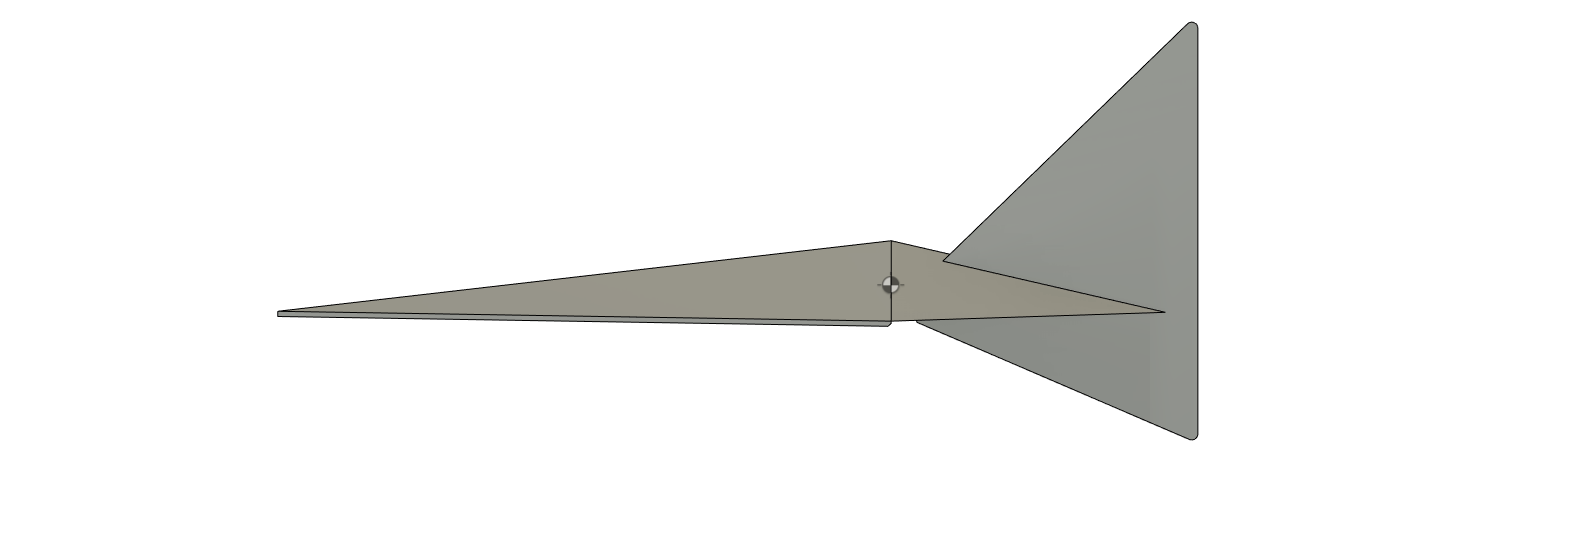
\includegraphics[width=0.75\linewidth]{assets/windsensor_top.png}
    \caption{Windflügel}
    
\end{figure}

Der Windflügel wird fest mit der Welle verbunden. Diese wird dann von oben ins leere Gehäuse geführt. Das Gehäuse weist dafür eine Öffnung auf, in welcher ein Kugellager verleimt wird, damit sich die Welle frei drehen kann. Die Konstruktion ist so ausgelegt, dass der Massemittelpunkt unabhängig von der Lage des Segelboots genau auf dem Drehpunkt des Windflügels liegt. Damit ist sichergestellt, dass auch bei den häufigen Schräglagen korrekte Werte ermittelt werden.

Das Gehäuse steht auf einer am Deck des Segelbootes gefestigten Grundplatte. Es hebt den Windflügel in den Wind und schützt die Adapterplatte mit dem Rotary-Hall-Encoder vor der Witterung und Wellen.


Der Windrichtungssensor wird an der Spitze des Bootes mit der Deckplatte verklebt.
\begin{figure}[H]
    \centering
    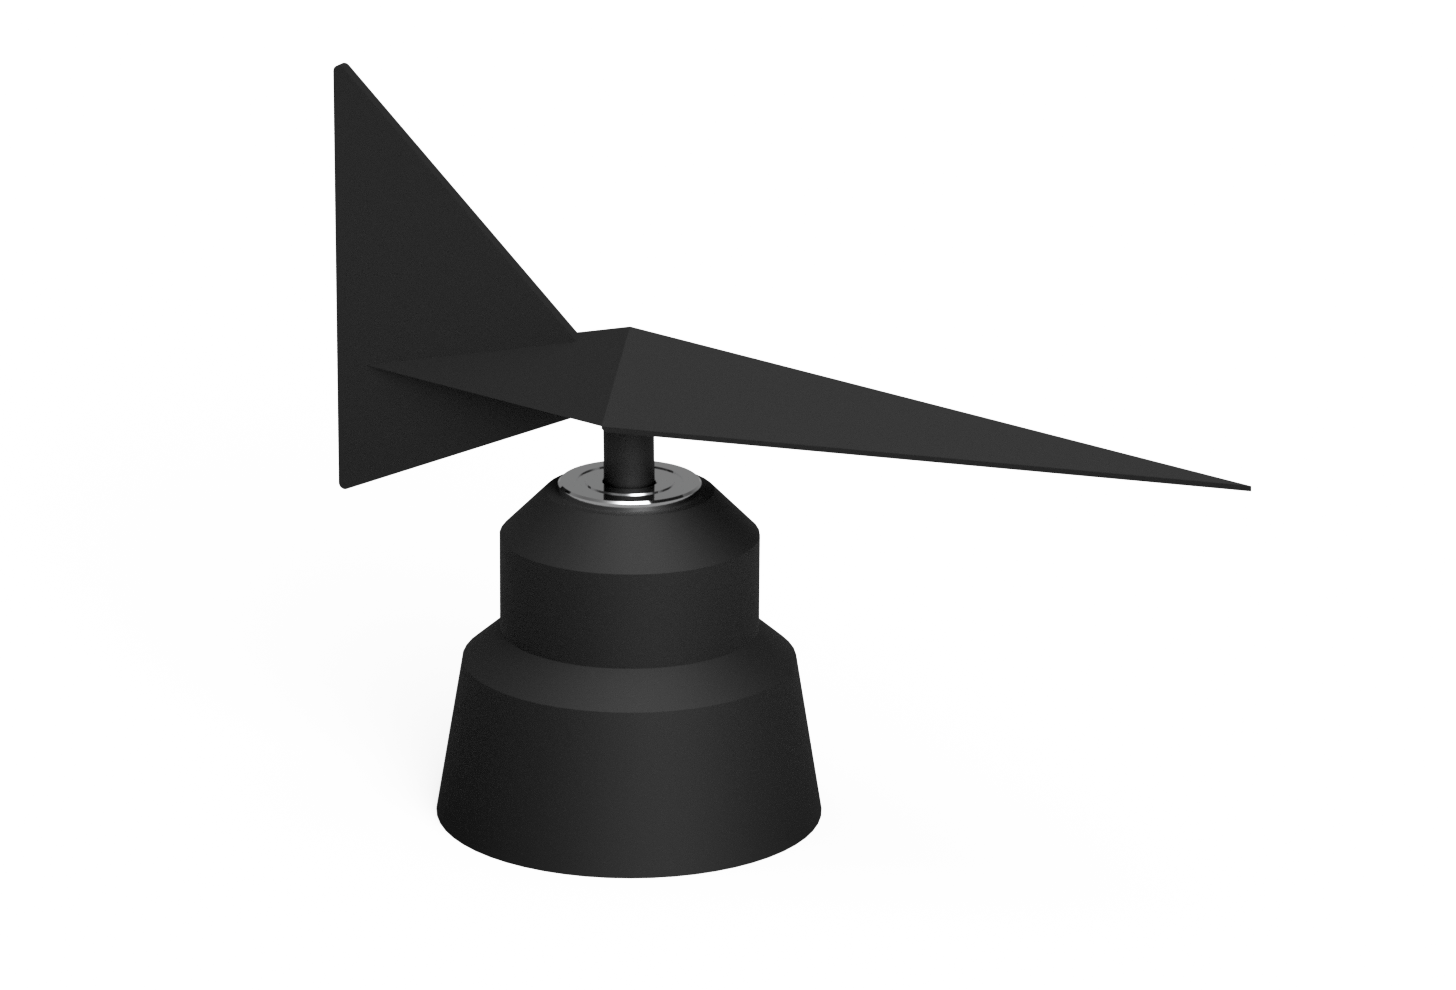
\includegraphics[width=0.75\linewidth]{assets/full_wind_sensor.png}
    \caption{Kompletter Windrichtungssensor}
    \label{fig:enter-label}
\end{figure}

\subsubsection{Aktuatoren}
Für die Bewegung des Ruders und des Sailflaps werden Aktuatoren verwendet. Aktuatoren (auch als Aktoren bezeichnet) sind das signalwandlerbezogene Gegenstück zu Sensoren. Sie setzen bei einem Bewegungsregelungsvorgang Signale durch mechanische Arbeit in Wirkungen um \cite{noauthor_aktor_2023}. Zur Bewegung von Ruder und Sailflaps werden elektrische lineare Aktuatoren benötigt. Ein elektrischer Linearantrieb ist ein Gerät, das die Drehbewegung eines Wechsel- oder Gleichstrommotors in eine lineare Bewegung umwandelt. Er kann sowohl Schub- als auch Zugbewegungen ausführen.

Für das vorliegende Projekt werden zwei L16-100-63-6 Serie R Aktuator der kanadischen Actuonix Motion Devices Inc. verwendet. Diese sind für den Einsatz in der Robotik und im Modellbau entwickelt worden und wasserdicht. Damit sind sie für den Einsatz auf Segelbooten prädestiniert.

Die Aktuatorwelle aus Aluminium verfügt über einem Maximalhub von 100 mm. Die Maximalgeschwindigkeit liegt ohne Last bei 20 mm/s. Damit sind sie nicht besonders schnell, verfügen mit 100N Stoss- und 46N Zugkraft aber über ausreichende Kraft zur Bewegung von Ruder und Sailflaps. Ihr Peak Power Point (der spezifische Geschwindigkeits- und Kraftpunkt, an dem die grösste Leistungsabgabe erfolgt) liegt bei 75N bei 10 mm/s. Das Getriebe der Aktuatoren weist eine Übersetzung von 63:1 auf.

\begin{figure}
    \centering
    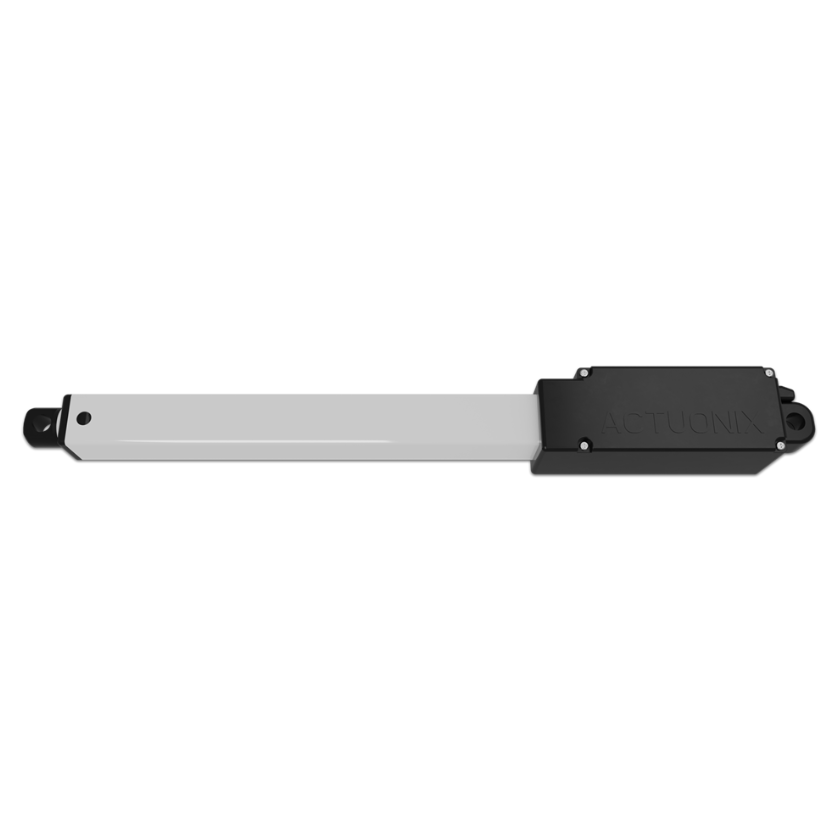
\includegraphics[width=0.75\linewidth]{actuonix.png}
    \caption{Actuonix Aktuator}
    \label{fig:actuator}
\end{figure}

Die Aktuatoren verfügen über kein digitales Positionsfeedback, das heisst, dass nicht abgefragt werden kann, an welcher Position sich das Ende der ausfahrbaren Welle befindet. Es können jedoch konkrete Distanzen angesteuert werden. 

Über eine einzige Datenleitung können kurze Impulse zwischen 1ms-2ms gesendet werden, wobei 1ms den Aktuator in die Startposition führt und der Aktuator bei 2ms voll ausgefahren wird. Um Einstellungen dazwischen zu erhalten, wird ein Wert zwischen 1ms und 2ms gesendet. 

Die Steuerleitung des Aktuators kann nicht direkt mit dem ESP32 verbunden werden, da dieser an seinen Pins nur 3,3 V Steuersignale ausgibt, der Aktuator aber ein 5 V Steuersignal erwartet. Aus diesem Grund muss zwischen den beiden Aktuatoren und dem ESP32 ein einfacher Pegelumsetzer (lever shifter) geschaltet werden. 
\begin{figure}[H]
    \centering
    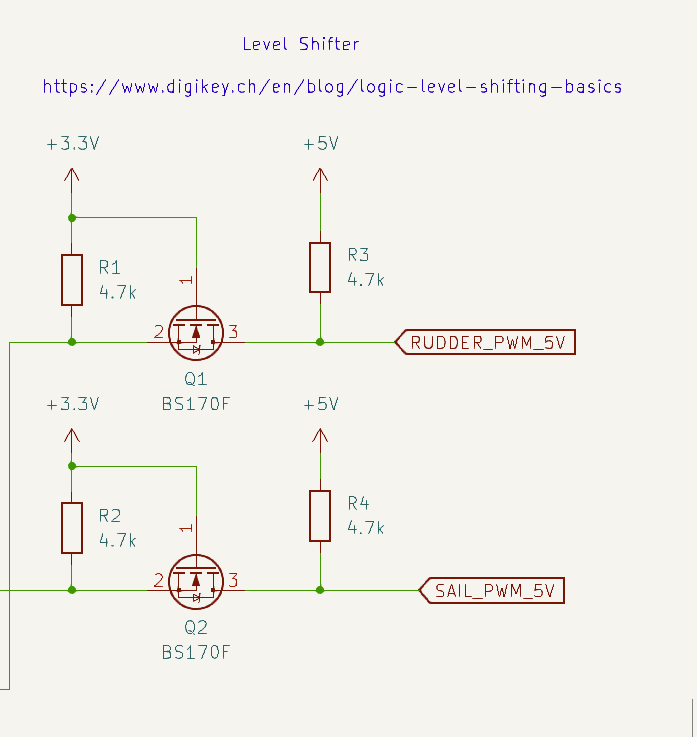
\includegraphics[width=0.5\linewidth]{assets/lvelshift.png}
    \caption{Schaltung Level Shifter von Sparkfun}
    \label{fig:enter-label}
\end{figure}

\subsection{Schleifring (Slip Ring)}
Der Aktuator zur Bewegung der Sailflaps muss an der Platine verkabelt sein. Da das Segel frei rotiert und sich um die eigene Achse drehen kann, besteht die Gefahr, dass die Verbindungskabel um den Mast gewickelt werden und reissen.

Dieser Gefahr kann mit dem Einsatz eines sogenannten Schleifrings begegnet werden.  Ein Schliefring ist ein elektromechanisches Bauteil, das eine elektrische Leistungs- oder Signalübertragung zwischen gegeneinander rotierenden Bauteilen ermöglicht. Er besteht aus einem stromleitenden Ring und Bürsten, die in Kontakt mit diesem Ring stehen. Die Bürsten bestehen aus einem leitfähigen Material und sind mit der stationären Struktur des Systems verbunden. 

Der Schleifring wird am Fuss des Segelmastes montiert und mit dem Schiffskörper verschraubt. Durch den hohlen Mast werden dann die drei Leistungen hinauf zum Segel gezogen und durch ein in den Mast gebohrtes Loch zum Aktuator geführt und mit diesem verbunden.


















\chapter{Software und Navigation}
\label{chap:navigation}
\section{Kurze Einführung ins Segeln}
Bevor man sich mit der autonomen Operation von Segelbooten beschäftigt, muss man zumindest in groben Zügen verstehen, wie und warum diese sich fortbewegen.
\subsection{Segelstellungen}
Grundsätzlich werden 5 Kurse bzw. Segelstellungen unterschieden.
\begin{itemize}
    \item Vorwind: Der Wind weht von hinten. (\textbf{U})
    \item Im Wind: Der Wind weht von Vorne.
    \item Halbwind: Der Wind trifft mit  $\pm$ 90$^{\circ}$ auf das Boot. (\textbf{U})
    \item Raumschot: Der Wind weht schräg von hinten. (\textbf{S})
    \item Amwind: Der Wind weht schräg von vorne. (\textbf{S})
\end{itemize}
Alle Kurse ausser der \textit{Im Wind} Kurs sind besegelbar. Dies liegt daran, dass dann, wenn der Wind von vorne auf das Boot trifft, dieser nicht vom Segel aufgefangen wird. Dieser Bereich wird als \textit{No Go Zone} bezeichnet und ist je nach Boot $\approx 90^{\circ}$. Auf den übrigen Kursen wird das Boot entweder durch das Stossprinzip (\textbf{S}), oder durch Umströmung (\textbf{U}) angetrieben. Bei der Umströmung wird derselbe Effekt genutzt wie bei den Flügeln von Flugzeugen. 
\subsection{Wahrer und scheinbarer Wind}
Es ist wichtig, zwischen dem wahren Wind und dem scheinbaren Wind zu unterscheiden. Der wahre Wind kommt aus der echten Richtung. Wer auf die Messdaten eines stationären Windsensors schaut, liest den wahren Wind ab. Der scheinbare Wind hingegen ist eine Zusammensetzung aus dem wahren Wind und dem Fahrtwind. Wenn im Segeln von der Windrichtung gesprochen wird, meint man in der Regel den scheinbaren Wind, da meist nur dieser von Bedeutung ist.
\begin{figure}
    \centering
    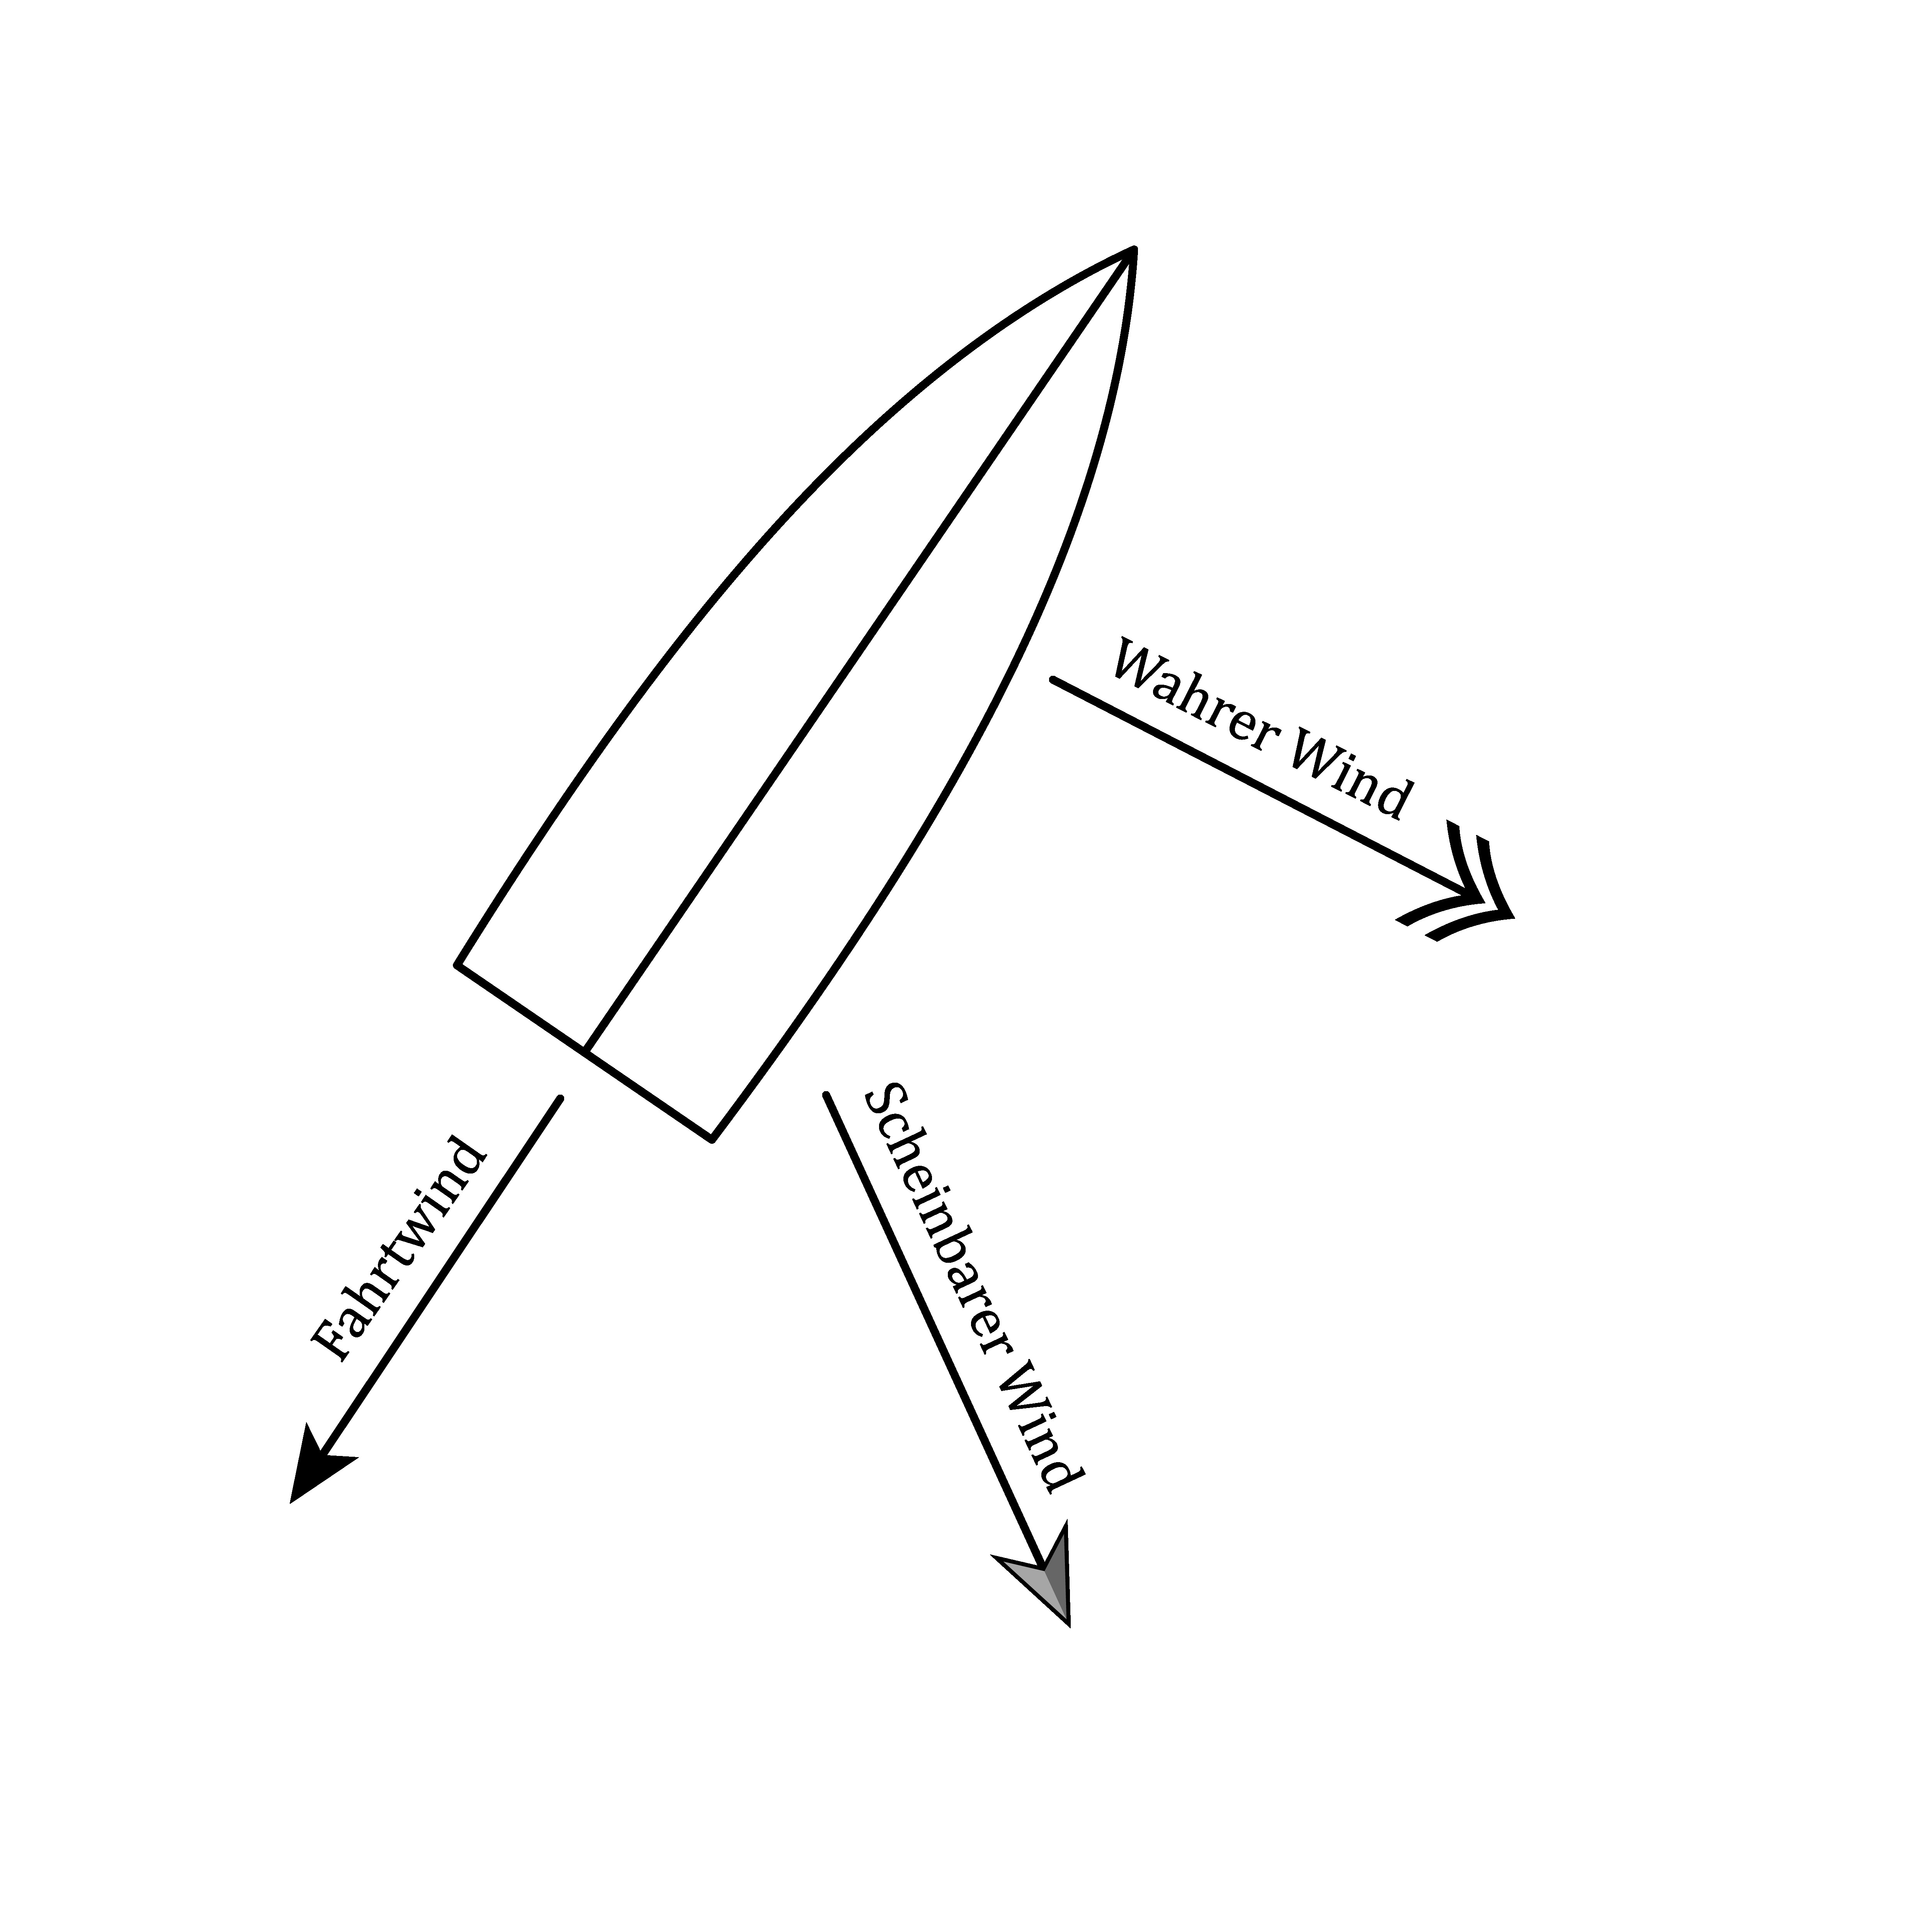
\includegraphics[width=0.75\linewidth]{assets/scheinbarerwind.png}
    \caption{Vektordarstellung des Windes}
    
\end{figure}

\section{Software}
\subsection{Programmiersprache}
Aufgrund der Anwendung auf einem ESP32 wurde das Program mit C++ entwickelt. In einer ersten Iteration ist Pyton auf einem Raspberry Pi gewählt worden. Aufgrund der mangelhaften Typisierung und der damit deutlich höheren Gefahr für Laufzeitfehler ist eine kompilierte Sprache hier angebracht. Ein Programmabsturz darf in einer solchen Anwendung nicht passieren weshalb die zuverlässigere Methode gewählt wird. 

Alternative Programmiersprachen wie Rust welche sich durch ihre Zuverlässigkeit auszeichnen haben eine deutlich kleinere Verbreitung.

Das Programm ist mit dem Arduino Framework und PlatformIO ertsellt worden. Dies vereinfacht das handhaben von mehreren Dateien und externen Bibliotheken.



\subsection{Aufbau der Software}
Die Architektur dieses Programms ist modular aufgebaut und besteht aus mehreren Klassen, die jeweils spezifische Aufgaben übernehmen. Die Hauptkomponenten sind:

\begin{itemize}
    \item \textbf{IMU}: Diese Klasse verwaltet die Inertial Measurement Unit (IMU) und stellt Methoden zur Initialisierung und Aktualisierung der Sensordaten bereit. Sie bietet auch Zugriff auf die Beschleunigungs-, Gyroskop- und Magnetometerdaten.
    \item \textbf{Actuator}: Diese Klasse steuert die Aktuatoren des Systems, insbesondere das Ruder und die Klappe. Sie bietet Methoden zur Initialisierung und Steuerung der Servos.
    \item \textbf{GPSManager}: Diese Klasse verwaltet das GPS-Modul und stellt Methoden zur Initialisierung und Aktualisierung der GPS-Daten bereit. Sie bietet auch Zugriff auf die aktuellen Positionsdaten, Höhe, Geschwindigkeit und Kurs.
    \item \textbf{BLEManager}: Diese Klasse verwaltet die Bluetooth Low Energy (BLE) Kommunikation. Sie initialisiert den BLE-Server und bietet Methoden zur Aktualisierung und Benachrichtigung von BLE-Charakteristiken.
    \item \textbf{Navigation}: Diese Klasse implementiert die Navigationslogik des Systems. Sie berechnet den optimalen Kurs basierend auf den aktuellen Positions- und Winddaten und steuert die Aktuatoren entsprechend.
\end{itemize}

Die Hauptlogik des Programms befindet sich in der \texttt{setup()} und \texttt{loop()} Funktion in der \texttt{main.cpp} Datei. In der \texttt{setup()} Funktion werden die verschiedenen Komponenten initialisiert, während in der \texttt{loop()} Funktion die Sensordaten regelmässig aktualisiert und die Navigationslogik ausgeführt wird. Die Kommunikation zwischen den Komponenten erfolgt über Singleton-Instanzen, die den Zugriff auf die jeweiligen Klassenmethoden ermöglichen.
Singleton wird gewählt, da somit ein Objektorientierter Ansatz auch für konkrete "Objekte" genutzt werden kann. Es ist somit aus der Programmstruktur klar, dass es nur ein spezifisches GPS Modul gibt.


\section{Webinterface für die Steuerung und das Monitoring des Segelboots}

\begin{figure}[H]
    \centering
    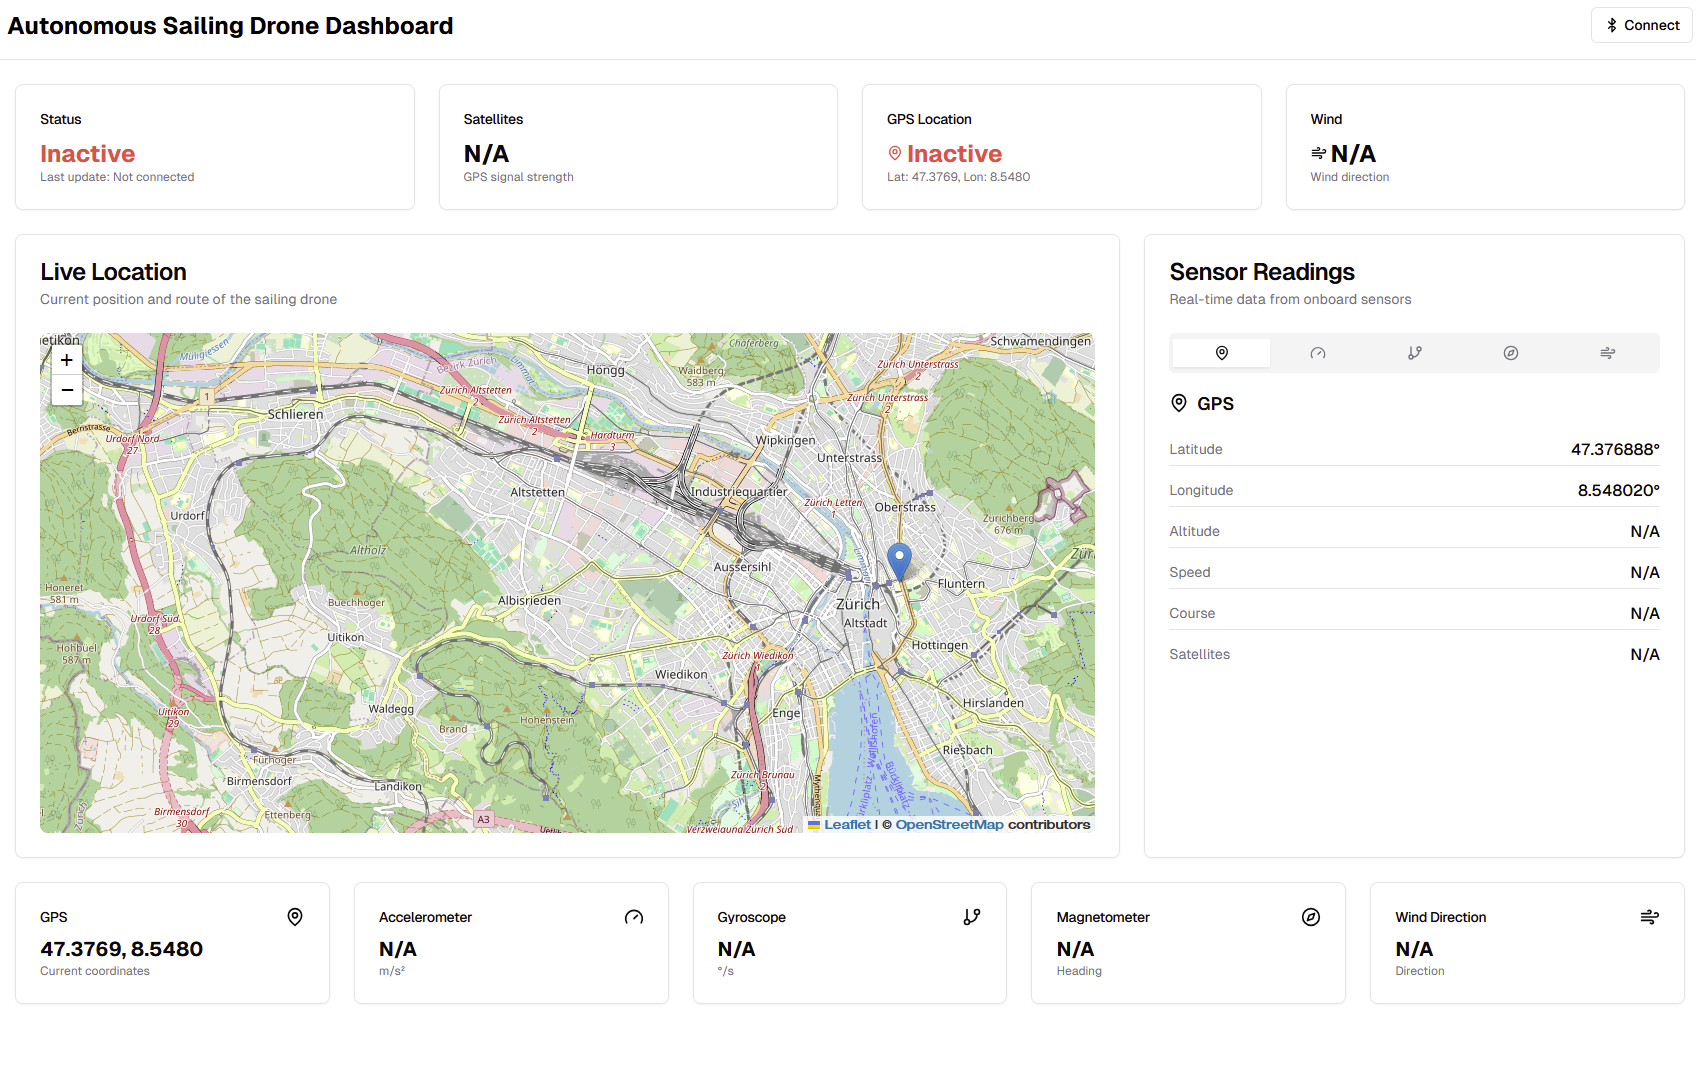
\includegraphics[width=1\linewidth]{assets/not cconnected interface.png}
    \caption{Dashboard (nicht aktiv)}
    \label{fig:enter-label}
\end{figure}

Um die Messwerte des Segelboots zu erhalten und dem Segelboot aus Distanz sein Ziel vorzugeben, wird ein Webinterface entwickelt. Diese macht sich die noch nicht weitverbreitete Implementierung der Web Bluetooth API zunutze. 

Das Segelboot verfügt über die Möglichkeit Daten über Bluetooth Low Energy (BLE) zu versenden. Dies ist, wie der Name bereits sagt eine Energiesparende Kommunikationsmethode die derzeit vor allem in Smarthome oder diversen Geräten wie Kopfhörer oder Tastaturen verwendet wird. Die Datenmenge die ausgetauscht werden kann ist relativ gering. Verwendet wird der Standard 4.2 der mit maximal 800 kbps keine grossen Datenmengen transferieren kann. 

Da dies für die Sensordaten nicht benötigt wird, kann auf viel Datentransfer verzichtet werden.


Die Möglichkeit über den Browser auf BLE Geräte zuzugreifen ist nicht weit verbreitet. laut mozilla.org wird dies derzeit nur von Chrome und Edge unterstützt. Aber auch bei diesen Browsern müssen zuerst die experimentellen Funktionen in den Einstellungen aktiviert werden.

Die Eigenschaft ohne Installation zusätzlicher Hardware am Computer, wie das bei den gängigen 433MHz Modulen der Fall wäre oder den erheblich höheren Energiebedarf der WLAN hätte, überwiegt die Einfachheit und Energieeffizienz von BLE. 

Aus dem Dashboard können folgende Werte Abgelesen werden.

\textbf{GPS-Navigationsdaten}
Die Positionsbestimmung erfolgt mittels eines satellitengestützten Navigationssystems mit folgenden Messgrössen:
\begin{itemize}
    \item \textbf{Breitengrad ($\varphi$):} Angabe in Dezimalgrad mit einer Präzision von $10^{-6}$ Grad
    \item \textbf{Längengrad ($\lambda$):} Angabe in Dezimalgrad mit einer Präzision von $10^{-6}$ Grad
    \item \textbf{Höhe ($h$):} Höhe über dem Meeresspiegel in Metern [m]
    \item \textbf{Geschwindigkeit ($v$):} Fortbewegungsgeschwindigkeit in Knoten [kn]
    \item \textbf{Kurs ($\alpha$):} Bewegungsrichtung in Grad [°] relativ zu geographisch Nord
    \item \textbf{Satellitenanzahl ($n_{\text{sat}}$):} Anzahl der empfangenen Satelliten zur Qualitätsbeurteilung des GPS-Signals
\end{itemize}

Die Signalqualität wird visuell durch Farbkodierung dargestellt: rot (inaktiv) bei $n_{\text{sat}} = 0$, gelb (eingeschränkt) bei $n_{\text{sat}} < 5$ und grün (aktiv) bei $n_{\text{sat}} \geq 5$.

\textbf{Beschleunigungssensor}
Der triaxiale Beschleunigungssensor erfasst die Beschleunigung in allen drei Raumrichtungen:
\begin{itemize}
    \item \textbf{X-Achse ($a_x$):} Beschleunigung in Längsrichtung in $\text{m}/\text{s}^2$
    \item \textbf{Y-Achse ($a_y$):} Beschleunigung in Querrichtung in $\text{m}/\text{s}^2$
    \item \textbf{Z-Achse ($a_z$):} Beschleunigung in Vertikalrichtung in $\text{m}/\text{s}^2$
\end{itemize}

\textbf{Gyroskop}
Das Gyroskop misst die Winkelgeschwindigkeit um die drei Raumachsen:
\begin{itemize}
    \item \textbf{X-Achse ($\omega_x$):} Rollrate in Grad pro Sekunde [°/s]
    \item \textbf{Y-Achse ($\omega_y$):} Nickrate in Grad pro Sekunde [°/s]
    \item \textbf{Z-Achse ($\omega_z$):} Gierrate in Grad pro Sekunde [°/s]
\end{itemize}

\textbf{Magnetometer}
Das Magnetometer dient zur Bestimmung der Ausrichtung relativ zum Erdmagnetfeld:
\begin{itemize}
    \item \textbf{Kurswinkel ($\psi$):} Ausrichtung in Grad [°] relativ zu magnetisch Nord
\end{itemize}

\textbf{Anemometer}
Der Windsensor liefert Daten zur Windcharakteristik:
\begin{itemize}
    \item \textbf{Windrichtung ($\theta_w$):} Richtung in Grad [°], aus der der Wind kommt
\end{itemize}

\textbf{Systemstatus}
Zusätzlich zu den Sensorwerten werden folgende Systemparameter überwacht:
\begin{itemize}
    \item \textbf{Verbindungsstatus:} Aktiv/Inaktiv je nach Bluetooth-Verbindungszustand
    \item \textbf{Letzte Aktualisierung:} Zeitstempel der letzten empfangenen Daten
\end{itemize}


Das Dashboard ist mit React und NextJs Entwickelt und verwendet die Ui Bibliothek von Vercel. Die Grundstruktur der Webseite wurde mit dem Ki Tool v0, welches ebenfalls von Vercel ist, generiert.





\section{Verbreitete Wegfindungsalgorithmen}
Für dieses Projekt wurden verschiedene Algorithmen auf ihre Eignung für dieses Projekt untersucht.

\subsection{Deep Reinforcement Learning Algorithm }
Deep Reinforcement learning ist ein Algorithmus aus der Familie des maschinellen Lernens. Seine Besonderheit ist, dass er im Gegensatz zum gewöhnlichen maschinellen Lernen keine Trainingsdaten benötigt. Hingegen wird ein \enquote{Agent} (vorliegend wäre das Segelboot der Agent) in eine virtuelle Umgebung gesetzt, in welcher er ein Ziel erreichen muss und dabei definierte Freiheitsgrade zur Bewegung hat. Wenn der Agent einen Fortschritt macht, wird dies belohnt. Macht er einen Fehler, wird er bestraft.

Der Nachteil dieses Algorithmus ist, dass er sich ausserhalb seiner trainierten Umgebung nicht zurechtfindet und dass die Bewegungen eines Segelboots sehr schwer in einer virtuellen Umgebung simuliert werden können. Eine auch nur ansatzweise akkurate Simulation würde den Rahmen dieser Arbeit eindeutig sprengen.
\subsection{Künstliche Potenzialfelder Algorithmus} 
Der Algorithmus der künstlichen Potenzialfelder ist eine Methode zur Pfadfindung, welche in der Robotik verbreitet ist. Der Algorithmus ermöglicht es, einen Weg zu finden, indem er auf anziehende und abstossende Felder reagiert, ähnlich wie dies in der Physik mit elektrischen Feldern geschieht.

Das Ziel des Algorithmus ist es, eine Richtung zu finden, in welche das Boot fahren soll, um vom Ausgangspunkt zu einem Zielpunkt zu gelangen. Dabei übt der Zielpunkt eine anziehende Kraft auf das Objekt aus, während Hindernisse eine abstossendend wirken entfalten. Mathematisch kann dies als Gradient dargestellt werden, bei dem die anziehende Kraft einen negativen Gradienten aufzeigt, der das Objekt zum Ziel zieht und die abstossende Kraft einen positiven Gradienten erzeugt, der das Objekt von Hindernissen abstösst.

Der gravierende Nachteil dieses Ansatzes ist, dass er in lokalen Minima stecken bleiben kann und tatsächlich auch stecken bleib. Überprüft wurde die Eignung des Ansatzes im Papier \enquote{Line following for an autonomous sailboat using potential fields method} \cite{inproceedings} . Dabei hat er sich auf offene Gewässer zwar als effizient erweisen, für engere Gewässer jedoch als ungünstig herausstellt.
\subsection{Vektor basierter Ansatz}


Die meisten der bekannten Algorithmen wurde mit Blick auf eine Überquerung
von Ozeanen oder die Navigation auf grossen Gewässern entwickelt. Dabei
spielen die Berücksichtigung von Wetterdaten etc. bei der Routenplanung
eine grosse Rolle. Für das vorliegende Projekt sind solche Thema aber nicht
relevant.
Es ist deshalb angezeigt, für das vorliegende Projekt einen eigenen Algorith-
mus zu entwickelt. Dieser basiert auf den Grundlagen der linearen Algebra
und lässt sich somit mit Gymnasialmathematik beschreiben. Ähnlich wie
beim Algorithmus der künstlichen Potenzialfelder wird bei jeder Berech-
nungsiteration der Kurs neu berechnet. Der Algorithmus hat eine gewisse
Ähnlichkeit zu demjenigen, welcher in A Simple Controller for Line Follo-
wing of Sailboats” beschrieben wird. \cite{sauze_simple_2013} Der Ansatz ist jedoch ganz anders
gewählt, daher ist die Ähnlichkeit vor allem in der Einfachheit. 


Der zentrale Algorithmus wird in der Methode \texttt{navigation\_step()} implementiert. Er wird in regelmässigen Abständen aufgerufen und entscheidet, wie das Boot seinen Kurs anpasst, um effizient zum nächsten Zielpunkt zu navigieren.

\subsubsection*{1. Vorbereitung der Daten}

Zunächst werden aktuelle Umgebungsdaten abgefragt:

\begin{itemize}
    \item \texttt{goal}: Zielposition als zweidimensionaler Vektor $(x, y)$, bestehend aus Längengrad und Breitengrad.
    \item \texttt{winddir}: Windrichtung in Grad, umgewandelt in Radiant.
    \item \texttt{currentHeading}: Kursrichtung des Bootes in Radiant.
\end{itemize}

Ausserdem wird die aktuelle Position des Bootes mit dem GPS abgefragt und als Vektor \texttt{currentPos} gespeichert.

\subsubsection*{2. Zielerreichung prüfen}

Das Boot überprüft, ob es sich bereits innerhalb eines Radius von 5 Metern um das Ziel befindet:
\[
\|\text{goal} - \text{currentPos}\| < 5
\]
Falls ja, werden Ruder und Flap auf neutral gesetzt.

\subsubsection*{3. Koordinatentransformation}

Die Windrichtung wird zunächst in ein lokales Koordinatensystem des Bootes transformiert. Dies erfolgt durch Anwendung einer Rotationsmatrix $R(\theta)$ mit dem Winkel des aktuellen Bootskurses:

\[
R(\theta) = 
\begin{bmatrix}
\cos(\theta) & -\sin(\theta) \\
\sin(\theta) & \cos(\theta)
\end{bmatrix}
\]

Die Transformation eines globalen Richtungsvektors (z. B. Windrichtung) in das Bootskoordinatensystem erfolgt durch:
\[
\vec{v}_{\text{lokal}} = R(\theta) \cdot \vec{v}_{\text{global}}
\]

So wird aus dem globalen Windvektor der relative Wind im Bootskoordinatensystem berechnet:
\[
\vec{v}_{\text{Wind,rel}} = R(\theta) \cdot \begin{bmatrix}\sin(\text{winddir}) \\ \cos(\text{winddir})\end{bmatrix}
\]

\subsubsection*{4. Prüfung auf Amwind}

Das Boot kann nicht direkt gegen den Wind segeln. Es prüft deshalb, ob der aktuelle Kurs in einem Bereich von ±45° zur Windrichtung liegt. Dies erfolgt durch das Skalarprodukt zweier normierter Vektoren:
\[
|\vec{v}_{\text{Boot}} \cdot \vec{v}_{\text{Wind,rel}}| < \cos(45^\circ) \approx 0{,}707
\]

Wenn diese Bedingung erfüllt ist, bedeutet das: Das Boot steht zu stark im Wind und muss einen Amwindkurs segeln.

\subsubsection*{5. Berechnung von Alternativkursen}

Zwei mögliche Amwindkurse werden generiert, indem zur Windrichtung jeweils ±45° addiert werden:
\[
\vec{v}_{\text{Option1}} = R(\theta) \cdot 
\begin{bmatrix}
\sin(\text{winddir} + 45^\circ) \\
\cos(\text{winddir} + 45^\circ)
\end{bmatrix}
\]
\[
\vec{v}_{\text{Option2}} = R(\theta) \cdot 
\begin{bmatrix}
\sin(\text{winddir} - 45^\circ) \\
\cos(\text{winddir} - 45^\circ)
\end{bmatrix}
\]

Diese Vektoren stellen mögliche Kurse dar, die den Wind in einem günstigen Winkel nutzen.

\subsubsection*{6. Auswahl des besseren Kurses}

Beide Kursoptionen werden mit dem Zielvektor verglichen, um zu bestimmen, welche Richtung effektiver ist. Hierfür wird wieder das Skalarprodukt verwendet:
\[
(\vec{v}_{\text{Ziel}} \cdot \vec{v}_{\text{Option1}}) 
\quad \text{vs.} \quad
(\vec{v}_{\text{Ziel}} \cdot \vec{v}_{\text{Option2}})
\]
Der Vektor mit dem höheren Wert zeigt stärker in Richtung des Zieles und wird daher gewählt.


\section{Kollisionsvermeidung}
Damit das Segelboot nicht auf Grund läuft, muss es über eine Funktion zur Kollisionsvermeidung verfügen. Diese funktioniert jedoch nur mit vorher einprogrammierten Hindernissen wie dem Ufer, Inseln, Sandbänken oder Naturschutzgebieten. 

Dabei wird dasselbe Prinzip angewendet wie dem Aufkreuzen (gegen den Wind fahren). Dabei wird bei jeder Iteration die Distanz zu den Hindernissen berechnet. Falls diese geringer als 40 m ist, erkennt das Boot diese als Gefahr und weicht ihnen aus.  

Hindernisse werden immer als Punkt behandelt. Grosse Hindernisse wie Inseln oder das Ufer müssen als eine Vielzahl von Punkten vorgegeben werden. Sobald Hindernisse in der unmittelbaren Nähe (40 m) des Bootes sind, erfährt die übliche Navigation die folgende Modifikation.

Als erstes werden die Vektoren zwischen den Hindernissen und dem Boot in einer Liste gespeichert. Beim Berechnen der neuen Richtung wird nun nicht mehr nur das Skalarprodukt zwischen dem Wind und dem Boot in Betracht gezogen, sondern ebenfalls das Skalarprodukt zwischen den einzelnen Hindernissen und dem Boot. So wird dann versucht, eine neue Richtung zu finden.

Die Nachteile dieses reaktiven Ansatzes sind offensichtlich. Das Boot könnte allenfalls in engen Buchten gefangen bleiben, weil es kein Weg aus diesen findet. Dies lässt sich aber dadurch vermeiden, dass dem Boot die Einfahrt in die Bucht durch ein entsprechendes Ziehen der Uferlinie grundsätzlich untersagt wird. 
\section{Motorsteuerung}
Wie im Kapitel Elektronik bereits ausgeführt, werden zwei Aktuatoren verwendet. Beide können mit einen einzigen 5 V Steuerimpuls in die eine gewünschte Position bewegt werden, wobei die genaue Position durch die Dauer des Impulses (zwischen 1 ms und 2 ms) bestimmt wird. 
\subsection{Ruder (PID Controller)}
Für das Ruder des Segelboots ist ein Regelungssystem notwendig, damit das Boot in die richtige Richtung gelenkt wird. Hierfür wird ein PD Controller verwendet. Der Name \enquote{PD} steht für Proportional (P) und Derivative (D). Diese Begriffe beschreiben die Hauptkomponenten des Regelungsalgorithmus. Der proportionale Teil des Reglers misst den Fehler zwischen der aktuellen Ausrichtung (des Bootes) und der gewünschten Ausrichtung. Dieser Fehler wird als Vektor dargestellt. Der P-Anteil multipliziert diesen Fehler mit dem Verstärkungsfaktor (Kp), um einen ersten Korrekturwert zu generieren. Demnach gilt, je grösser der Fehler ist, desto grösser muss die Korrektur sein. Mit diesem Teil des Reglers wird das Ruder erstmals in die richtige Richtung gelenkt. Der Derivativteil (D) des Reglers achtet darauf, wie sich die Änderung des Fehlers verhält. Wenn das Boot sich dem gewünschten Kurs nähert, kann der Fehler schnell abnehmen, was zu einem Überschwingen führen kann. Der D-Teil versucht, dieses Überschwingen möglichst zu reduzieren, indem er den Fehlergeschwindigkeitsvektor (sprich die Ableitung des Fehlers) berechnet. Dieser wird ebenfalls mit einem Verstärkungsfaktor multipliziert. Aus der Kombination von P- und D-Komponenten kann eine Ruderposition, die zwischen 0 und 1 liegt, berechnet werden. Ein Wert von 0.5 entspricht dem Ruder, welches sich, wenn alles stimmt, in der Mitte befinden sollte. Somit kann sich das Boot sanft an den gewünschten Kurs annähern, ohne dauernd zu übersteuern. 
\subsection{Segel}
Da das Segel kann wie im Abschnitt \ref{sec:sailflap} \nameref{sec:sailflap} bewegt werden. Da die Schnelligkeit des Bootes bei dieser Arbeit untergeordnet ist, wird das Sailflap immer in die Richtung des Windes gedreht. Dies sorgt dafür, dass das Segel in eine segelbare Position geführt wird. Diese wird in den meisten Fällen nicht optimal sein  jedoch ausreichend für diesen Anwendungsfall.
\begin{figure}
    \centering
    \includegraphics[width=0.75\linewidth]{sailflap_erklärung.png}
    \caption{Sailflap Visualisierung}
    \label{fig:enter-label}
\end{figure}


\chapter{Herstellung und Zusammenbau}
\label{chap:herstllung}

\section{Herstellungsprozess der Komponenten}
\subsection{Skelett und grundlegende Bootsform}
Da für dieses Projekt keine computergesteuerte \ac{cnc} Fräse zur Verfügung steht, werden die Spanten des Bootes mittels einer elektrischen Handstichsäge aus drei verleimten Tannenbrettern mit den Massen 240 mal 40 cm und einer Stärke von 18 mm ausgesägt. Dafür werden die Baupläne der zehn Elemente mithilfe eines Plotters im Massstab 1:1 ausgedruckt und  mit Hilfe von transparentem Backpapier mittels der Abpausmethode auf Tannenholzbretter übertragen, und anschliessend mit der Handstichsäge ausgesägt.

Die Erstellung der Spanten erfolgt in zwei Arbeitsschritten. Im ersten Schritt wird die äussere Form ausgesägt. In einem zweiten Schritt wird danach Material von innerhalb der Elementen entfernt. Dies wird aus Gewichtsgründen gemacht und schafft den für die spätere Montage der Elektronik und der Energieversorgung notwendigen Freiraum im Inneren des Bootes.

An den entsprechenden Stellen an der Oberseite der Elemente werden je zwei Löcher gebohrt und die Elemente werden dann mithilfe zweier Aluminiumstangen ineinander befestigt. Um eine Verschiebung der Elemente während des Herstellungsprozess zu vermeiden wird Heisskleber verwendet. 
\begin{figure}[H]
    \centering
    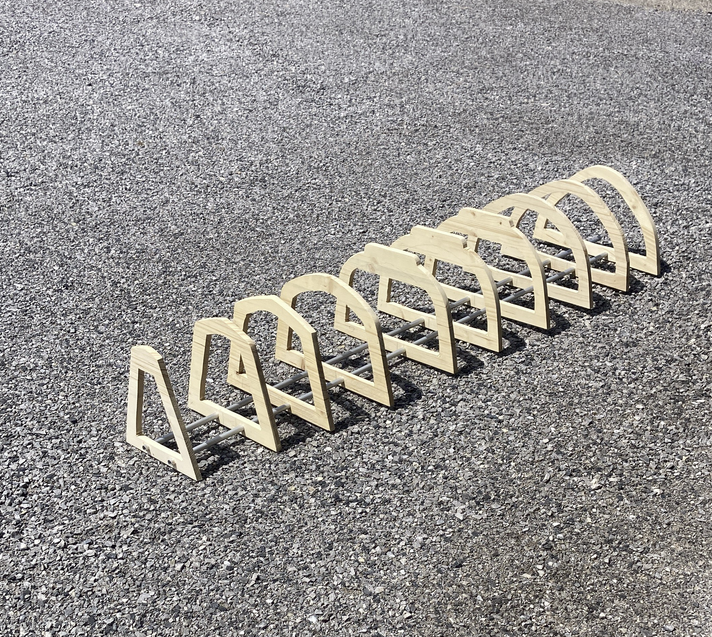
\includegraphics[width=1\linewidth]{rippe1.png}
    \caption{Rippen förmige Anordnung der Tragelemente}
    \label{fig:enter-label}
\end{figure}

Da die Spanten  mit einer Handstichsäge ausgesägte werden, lassen sich  Ungenauigkeiten nicht völlig vermeiden. Daher weichen die tatsächlichen Masse der Spanten bis zu 5 mm von den Planwerten ab. Obwohl dies eine relative Abweichung ist, kann der Fehler in den folgenden Arbeitsschritten ausgebessert werden. 

Da für die Elemente aus Kostengründen kein Massivholz genommen werden kann, muss auf Leimholz zurück gegriffen werden. Dies hat zum Nachteil, dass einzelne Elemente einen Bruch erleiden, wenn zu viel Druck auf die geleimten Stellen wirkt. Beschädigte Elemente werden nicht verwendet sondern durch neu  erstellt Kopien ersetzt. 
\begin{figure}[H]
    \centering
    \includegraphics[width=0.25\linewidth]{bruch.png}
    \caption{Bruch eines Elements}
    \label{fig:bruch}
\end{figure}

Im Anschluss wird eine Schicht Balsaholz über die Rippen gelegt. Die verwendeten Balsaholzbrettchen haben eine Stärke von 1mm und sind 100 cm lang. Zur Befestigung an den Spanten wird eine Tackerpistole verwendet. Durch Verspannungen im Holz ergeben sich unglücklicherweise kleinere Verformungen, welche sich negative auf die endgültige Bootsform auswirken können.

\subsection{Glasfaserbeschichtung}
Um eine robuste  Aussejnhülle für das Boot zu schaffen, wird eine glasfaserverstärlte Epoxidharzschicht  aufgetragen. Die Verbndung von Glasfasermatten mit Epoxidharzergibt eine äusserst harte und stabile Schicht.  Dafür  werden die Glasfasermatten auf die Balsaholzplanken gelegt und mit Epoxidharz bestrichen. Dies führt dazu, dass die Epoxidschicht die Form des Bootes animmt. Das unterliegende Balsaholz bildet also  die formgebende, und die Glasfaser-Epoxidschicht die  strukturgebende Komponente. 

Dieses Vorgehen führt jedoch auch zu Problemen, da der Auftrag der Glasfaser-Epoxidschicht zu Verspannungen in der Balsaholzschicht führt. Auch die Schwankungen des Feuchtigkeit in der Werkstatt bewirken Verspannungen, welche sich dann ebenfalls auf die Balsaholzschicht auswirken.  Um diese Dellen in der Auseenhülle auszugleichen, muss sehr viel Expoxidspachtemasse aufgetragen wird. Dafür wird eine Mischung von Expoixid und entsprechendem Härtungsmittel verwendet.  Um das folgende Planschliefen der Oberfläche zu vereinfachen, werden diesem Gemisch Microballons beigemischt und ein Tixotropiermittel wird zugegeben, um das Gemisch einzudicken. Der Prozess des Auftragens und Abschliefens muss  viele Male wiederholt werden. Das ist sehr zeitaufwändig, da immer gewartet werden muss, bis die neu aufgeragenene Schicht vollständig ausgetroknet ist.  Dabei wird  versucht wird einen möglichst glatten, stromlinienförmigen Körper zu formen.

Um eine Asymetrie beim Bug zu vermeiden, wird sehr viel Expoxid-Spachtelmasse augetragen. Kleine Glasfaserschnippsel, welche zu Spachtelmasse dazugerührt werden, geben dieser weitere Stabilität, damit der Bug gut geschützt ist.
\subsection{Ruder}
Das Ruder wird aus einer Tannen-Leimholz Platte ausgesägt. Dabei wird daselbe Verfahren wie bei den Spanten angewendet. Anschliessend wird das Werkstück mit der Schliefmaschine bearbeitet und in Form gebracht. 

Nach der Lackierung mit roter Farbe wird das Ruder am Heck des Schiffskörpers befestigt und mit der Welle des Aktuators verbunden.
\subsection{Kiel}
In einem ersten Schritt werden die 5 Bretter ausgesägt, mit einander verleimt und verschraubt. Anschliessend werden in die Löcher für die Gewindestangen in die beiden äusseren Kielbretter gebohrt. 

Im nächsten Schritt wird ein Loch in die beiden 2 Kg Gewichte gebohrt. So können die Gewichte mit dem Kielhauptbrett verschraubt werden. Nach dem Druck der beiden Schutzgehäuse werden diese über die Gewichte gestülpt und mit dem Kielhauptbrett verleimt.    
\begin{figure} [H]
    \centering
    \includegraphics[width=0.3\linewidth]{assets/Kiel_lakiert.png}
    \caption{Fertiger Kiel}
    \label{fig:enter-label}
\end{figure}

\subsection{Segel}
Das Segel besteht aus EPS und setzt sich aus vier identischen Teilen zusammen, die aus EPS-Platten ausgeschnitten werden. Je zwei Platten bilden die rechte und die linke Seite des Segels, das eine aerodynamisch günstige Form aufweist. Dazu werden die beiden Segelhälften verklebt.  
\subsubsection*{EPS Schneidgerät}
Mit speziellen Schneideräten können Formen aus EPS Platten geschnitten werden. Konventionelle EPS Schneidgeräte sind allerdings nicht genügend gross, um dien vier Teile auszuschneiden, weshalb ein eigenes Schneidgerät gebaut werden muss. Alle EPS Schneidegeräte funktionieren nach demselben Prinzip. Dabei wird ein Metalldraht  auf  60$^\circ$ C - 100$^\circ$ C) erhitzt und ins EPS gefahren, wo dieses lokal zum Schmelzen gebracht wird. Indem der Draht durch den EPS Körper gezogen wird, entsteht damit ein sauberer Schnitt. Der Draht wird dadurch erhitzt, dass an ihn eine elektrische Spannung gelegt wird. Der Draht bildet einen Widerstand und wird hiess.. Der Draht ist so ausgelegt, dass er einen möglichst hohen Wiederstand aufweisst. 

Damit die  vier grossen Segelteile als ganzes aus EPS Blöcken geschnitten werden können, wird ein eigenes einfaches Schneidegerät mit entsprechenden Dimensionen gebaut.  Dazu wird ein sogenannter \enquote{Wiederstandsdraht} mit einem Durchmesser von $\varnothing$ 0.2mm gekauft. Dieser wird dreifach Verdrillt und daraus ein Schneidedraht mit einer Länge von 1.5 m erstellt. Die beiden Enden werden in einen U-förmigen Rahmen aus Tannenholzlatten gespannt. Als Stromquelle dient zunächst ein Labornetzteil, das 3A bei 12V liefert. 

Die ersten Versuche, zunächst noch mit einem einfache, und anschliessend mit einem zweifachen Draht verlaufen erfolglos. Erst als eine dreifach verdrillter Draht und ein stärkeres Labornetzteil, das 5A bei 12 V liefert, verwendet werden, wird der Draht soweit aufgeheizt, dass damit EPS geschnitten werden kann.     


\begin{figure}[H]
    \centering
    \includegraphics[width=0.5\linewidth]{foamcutter1.png}
    \caption{Foamcutter}
    \label{fig:enter-label}
\end{figure}

\subsubsection*{Grosssegel}
Um die geplante Form aus den \ac{eps} Platten schneiden zu können, wird zuerst mithilfe eines Lasercutters eine Halbprofilform aus Sperrholz erstellt. Je eine solche Halbprofilform wird mit zwei  Schraube an den beiden kürzeren Seiten einer EPS Platte  befestigt . Der heisse Schneidedraht kann damit entlang der Kante der Halbprofilschablone durch den EPS Block gezogen werden. So entsteht ein halbes Segel mit der Form der Halbprofilschablonen . \\


\begin{figure}[H]
    \centering
    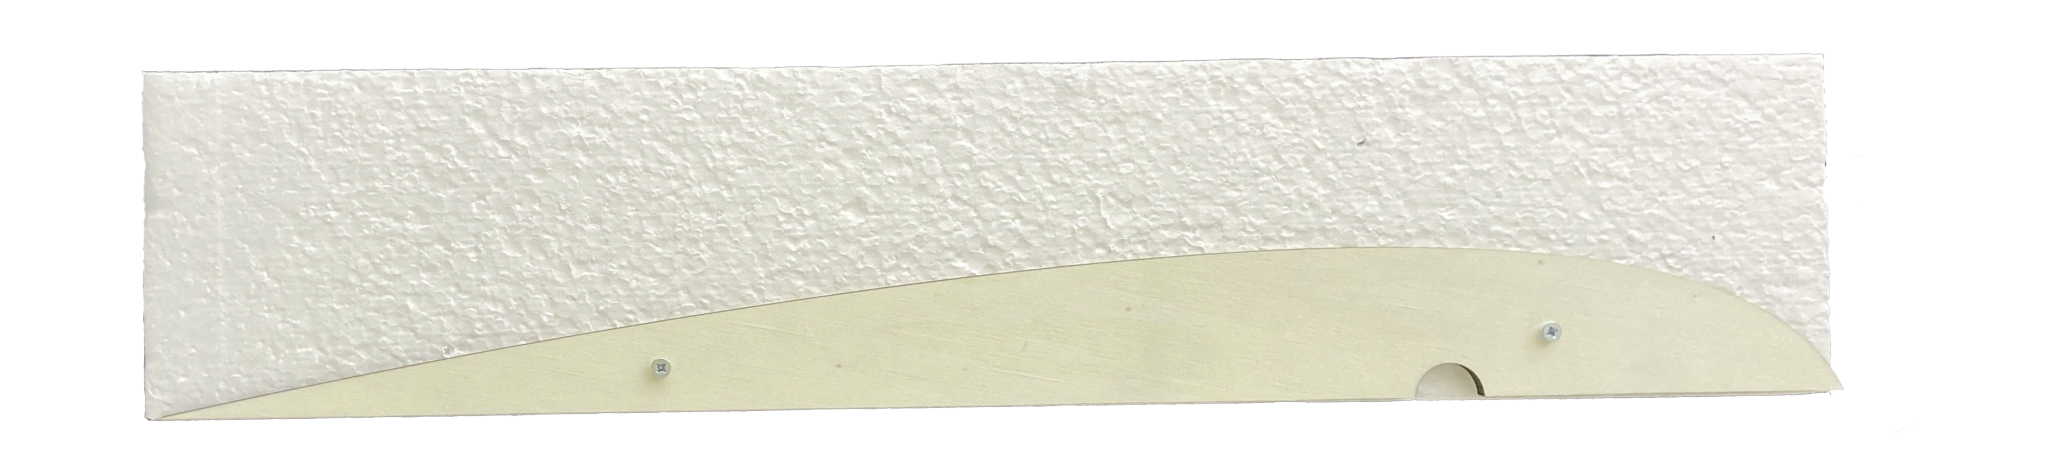
\includegraphics[width=1\linewidth]{assets/template_on_foam.png}
    \caption{Seitenansicht eines Elements mit der Schablone}
    \label{fig:enter-label}
\end{figure}

Anschliessed muss auf der planen Seite des Halbsegelteils noch eine halbrunde Kerbe ausgeschnitten werden. In ihr findet bei der Verleimung der Platten der Aluminiummast platz. Nicht jeder Schneidversuch verläuft erfolgreich. Wenn die beiden Enden des Schneiddrahtes nicht synchron über die Halbprofilform geführt werden, oder wenn dieser nicht präzis gefolgt wird, weist der ausgeschnittene Körper erhebliche Formfehler auf. Auch bei einem an sich erfolgreichen Schnitt ergeben sich aber kleine Ungenauigkeiten, die aber mit einem Schliff des Bauteils korrigiert werden können. 

Nachdem erfolgreich vier Profile ausgeschnitten worden sind, wird der Mast in die ausgesparte Kerbe gelegt und fixiert. Danach werden die vier Profile in Paaren verklebt.      

\subsection{Saailflap}
Das Sailflap wird mit der selben Technik wie das Grosssegel hergestellt. Es wird mit zwei Carbonstäben am Grossselgel fixiert. In einem letzten Schritt wird der Aktuator ins Grosssegtel einbebaut und mit dem Sailflap verbunden.   
\section{Bemalung}
Da das autonome Segelboot gut sichtbar sein soll, wird es in roter Signalfarbe bemalt. Dazu wird seidenmatter Acryllack verwendet, der mithilfe einer Farbwalze auf den Bootskörper aufgetragen wird. Es wurde bewusst  eine matte Farbe  gewählt, da diese kleine Ungenauigkeiten und Dellen in der Bootsform besser kachiert als glänzende Farben. 

Da das Rudern, der Kiel und das Deck keine Schützhülle aus glasfaserverstärktem Epoxidharz verfügen, dient hat die Farmlackierung bei diesen Bauteilen auch eine Schutzfunktion.
\section{Einbau der Elektronik}
Als erstes wird ein digitaler Schaltplan mit allen Sensoren und Aktuatoren und Sensoren erstellt. Dieser dientals Bauanleitung für den Bau. Die für die Erstellung des Schaltplan notwendigen Informationen werden den Datenblättern der Geräte und  Sensoren entnommen, in denen ihre Funktionsweise beschrieben und die Betriebsweise erläutert werden.
\subsection{Raspberry Pi}
Der Raspberry Pi Zero W 1.1 wird direkt über seinen 5V Pin angesteuert. Zwischen den Energiespeicher und dem Rapberry Pi iZero W 1.1 wird ein Spannungswandler geschaltet, der die ca. 7V Ausgangsspannung des Energiespeichers auf 5V reduziert.

Diese Vorgehensweise hat den Nachteil, dass dass der Raspberry die gesamte Schutzelektronik, welche beim USB Port angebracht ist, überspringt. Der bedeutende Vorteil ist jedoch, dass verlötete Verbindungen  permanent sind und diese sich ohne erhbeliche Gewalt bei Normaltemperaturen nicht lösen. Bei einem sich durchgehend bewegten System ist dies notwenig. 

Ein Ausfall der Bordelektronik würde für das Boot katastrophal enden. 
\subsection{Aktuatoren}
Wie im Kapitel \enquote{Elektronik} bereits erläutert, verfügen die verwendetet Aktuatoren über 3 pins. V+, GND und einen Datapin. 

Da der Raspberry Pi Zero W 1.1 über seine 5V output pins nicht genügend Leistung für das Ansteuern eines, und schon gar nicht von den mehrerer Aktuatoren verfügt, werden diese direkt mit dem Stromversorgung verbunden. Da die Geräte über eine gemeinsamen Groundleitung \enquote{common Ground} verfügen, kann der Raspberry Pi Zero W 1.1 den Aktuator dennoch ansteuern. 

Ein weiteres Problem ergibt sich daraus, dass an den Datenpins des Raspberry Pi Zero W 1.1 nur Steuersignale von 3.3V ausgegeben werden, der Aktuator aber ein 5V Steuersignal benötigt. Der Aktuator kann damit nicht direkt vom Raspberry Pi Zero W 1.1 ansteuert werden. Dieses Problem lässt sich aber einfach  ösen, indem ein Pegelumsetzer zwischengeschaltet werden. 


\chapter{Tests und Leistungsbewertung}
\label{chap:tests}


\section{Prüfung der mechanischen Eigenschaften}
Nach ausreich

\section{Funktionalität der Sailflap-Technologie}

\section{Autonome Navigationstests}



\chapter{Ergebnisse und Diskussion }
\label{chap:diskussion}
Test 123

\section{Zusammenfassung der Ergebnisse}
\section{Bewertung des autonomen Segelschiffs}
\section{Diskussion von Herausforderungen und Verbesserungspotenzial}


\chapter{Fazit}
\label{chap:fazit}


\section{Bewertung des autonomen Segelschiffs}




\section{Diskussion des Verbesserungspotenzials}
\subsection{Rumpf}
Bei einer Wiederholung des Bootsbaus würde die Konstruktion und der Bau des Rumpfes anders erfolgen. Die Verwenden von 3D- gedruckten Elementen hat sich beim Spitz als sehr erfolgreich herausgestellt. Daher würde bei einem zweiten Bau auf die Balsaholzbeplankung verzichtet werden und dafür möglichst lange und breite 3D-gedruckte Elemente verwendet. Diese würden mit der CAD Software entworfen und in der idealen Form gedruckt. Damit  würden Verspannungen im Holz und die daraus resultierenden Ungenauigkeiten  vermieden werden, die im daran anschliessenden Arbeitsschritt, der Beschichtung mit glasfaserverstärktem Epoxiharz sehr viel und zeitaufwendige Arbeit verursacht hat.

Sodann würden Spanten von geringerer Stärke, dafür in grösserer Zahl vorgesehen. Diese Spanten könnten dann mit dem Lasercutter erstellt werden.  
\subsection{Elektronik}
Bei einer Wiederholung des Bootsbaus sollte für die Verkabelung der elektronischen Bauteile eine Platine individuell entworfen und bei einem Auftragsfertiger in Auftrag gegeben werden. Der Aufbau und die Fehlersuche würde damit enorm erleichtert. Auch könnte der Aufbau damit sehr viel ordentlicher vorgenommen werden.

Sodann sollte ein wasserdichtes Gehäuse entworfen und gebaut werden, in dem der Raspberry Pi Zero W 1.1, die Platine, und der Pegelumsetzer Platz finden. Auch für den Energiespeicher und die Ladeelektronik sollte ein wasserdichtes Gehäuse entworfen und gebaut werden. Damit könnte die Gefahr eines Kurzschlusses bei einem Wassereinbruch, z.B. bei hohem Wellengang, stark reduziert werden.
\subsection{Segel}
Bei einer Wiederholung des Bootsbaus sollten im Mast zwei Löcher zur Verankerung der Carbonrohre vorgesehen werden, an welchen das Sailflap montiert wird. 

Die Oberfläche des Grosssegels und des Sailflaps würde mit einer dünnen Schicht glasfaserverstärktem Epoxidharz geschützt. 
\subsection{Kiel}
Bei einer Wiederholung des Bootsbaus sollte der Kiel aus Massivholzbrettern statt verleimten Platten aufgebaut werden, um die Gefahr eines Bruchs bei übermässigem Seitendruck oder einer Grundberührung weiter zu vermindern. Ausserdem sollte der Kiel mit einer dicken Schutzschicht aus glasfaserverstärktem Epoxidharz eingefasst und geschützt werden. 
\subsection{Ruder}
Bei einer Wiederholung des Bootsbaus würde das Ruder nicht am Ende des Bootskörpers vorgesehen, sondern vollständig unter Wasser am Heck des Bootskörpers befestigt und über eine Welle bewegt werden, die den Bootsboden verikal schneidet. Damit könnten für die Rudersteuerung ein einfacher und günstiger  Servomotor im Schiffskörper montiert und betrieben werden. Der zuverlässigen Abdichtung der Wellendurchführung müsste dabei grosse Aufmerksamkeit geschenkt werden. Ausserdem würde das Ruder im 3D-Druckverfahren hergestellt. 
\section{Ausblick auf zukünftige Entwicklungen im Bereich der autonomen Segelboote}
Autonome Segelboote werden nie dieselbe Aufmerksamkeit wie autonome Landfahrzeuge auf sich ziehen. 

Ihre Einsatzmöglichkeiten sind begrenzt. Dies finden sich vornehmlich in Nischen. Da Windstärke und Richtung auf absehbare Zeit nicht zuverlässig prognostiziert werden können, sind weder Reiserouten noch Reisezeiten autonomer Segelboote zuverlässig planbar oder auch nur annäherungsweise prognostizierbar. DAs setzt einem kommerziellen Einsatz enge Grenzen. Eine weite Verbreitung autonomer Segelboote darf daher nicht erwartet werden. 

Autonome Segelboote könnten aber beispielsweise im Monitoring von Gewässern ein wichtiges Instrument werden, um grosse Räume über längere Zeiträume kostengünstig zu überwachen. Dabei ist zwischen dem maritimen Einsatz und dem Einsatz auf Binnengewässern zu unterscheiden. 

Für den maritimen Einsatz werden sich deutlich grössere Boote als das in diesem Projekt erstellte Boot durchsetzen. solche eigenen sich ideal für Monitorinaufgaben in abgelegenen Meeresgegenden wie dem Südpolarmeer oder Teilen des indischen und pazifischen Ozeans., da sie ohne weiteres mehrere Monate oder gar wenige Jahre im autonomen Einsatz stehen können. Damit könnten beispielsweise Erkenntnisse über die Entwicklung von Fischpopulationen, die Wasserqualität oder Wassertemperatur, die Vermüllung aber auch Wetterdaten gewonnen werden. 

Der Einsatz von autonomen Booten der Grössenordnung wie in der  vorliegenden Arbeit auf dengrossen Schweizer Seen ist wenig wahrscheinlich, da diese von einer Vielzahl von Freizeitbooten befahren werden, die eine Gefahr für das autonome Segelboot darstellen. Viel eher ist an einen Einsatz solcher Boote auf den zahllosen Seen in den nordischen Ländern zu denken, die in sehr dünn besiedelten Gegenden liegen, und bei denen kaum eine Infrastruktur vorhanden ist, die eine gleichwertige Überwachung auf andere Weise erlauben würde.


\chapter{Danksagung}
\label{chap:danksagung}
Das Projekt hätte ohne die wertvole Hilfe der vieler Personen nicht realisiert werden können. Ausdrücklich hervorheben möchte ich
\begin{itemize}
\item Thomas Zwick, mein Segellehrer, der mir als Fünjährigem meine ersten Segelstunden erteilt. Er hat mich nicht nur zum  Segeln gebracht, sondern hat mir für den Bau des Segelbootes in grosszügiger Weise seine Werkstatt zur Verfügung gestellt und mich zunächst in die Technik der Arbeit mit glasfaserverstärkten Kunststoffen eingeführt und danach bei diesen Arbeiten tatkräftig untersützt hat.
 \item Dr. Carola Ebenhoch, meine Betreuerin und ehemalige Physiklehrerin, welche mir bei dieser Arbeit sehr viel Freiraum eingeräumt, meine etwas waghalsige Idee ein komplettes Segelboot zu entwerfen, konstruieren und zu bauen gelassen hat.
  \item Raphael Barengo, ebenfalls Physiklehrer an der Kantonsschule Uetikon am See, der mir Zugang zu den 3D Druckern, dem Lasercutter und diveresen anderen Werkzeugen in der Makerhall der Schule ermöglicht hat.  
  \item Samuel Achermann, mein Mathematiklehrer an der Kantonsschule Uetikon am See, der sich in den Ferien Zeit genommen, mit mir Navigationsalgorithem durchzudenken und mir vor allem dabei geholfen hat, den Potential Fields Algorithmus zu verstehen.
  
  \item Gian-Andri Morf, mein Cousin und MSc ETH Masch. -Ing., von dem ich am Anfang des Projekts sehr viel zur Materialauswahl lernen konnte.
  \item Meine Mutter, welche mich während des ganzen Projektes geduldigst unzählige Male in die Werkstatt gefahren und von dort wieder abgeholt hat.
  \item  Mein Vater, den ich als Lektor missbrauchen durfte und der mich bei den rechtlichen Aspekten beraten hat.
   \item Samuel Hasenfratz, Mitarbeiter und Ingenieur bei Tribecraft AG, Zürich, der mir nicht nur das spannende Unternehmen vorgestellt, sondern sich auch viel Zeit genommen hat, einige Herausforderungen, vor allem bezüglich der Navigation die noch zu lösen waren, zu durchdenken oder gar eine Lösung zu finden. 
\item Distrelec Schweiz AG, Nänikon, die sich bereit erklärt haben, mein Projekt mit einer grosszügigen Sachspende in Form von elektronischen Bauteilen zu unterstützen. 
 
\end{itemize}


%\printglossary
%

\newacronym{cnc}{CNC}{Computerized Numerical Control}
\newacronym{cad}{CAD}{Computer Aided Design}



\newglossaryentry{luv}
{
    name=luv,
    description={Wind zugewandte Seite}
}

\newglossaryentry{lee}
{
    name=lee,
    description={Wind abgewandte Seite}
}
\newglossaryentry{backbord}
{
    name=backbord,
    description={Vom Boot nach vorne schauend Links}
}

\newglossaryentry{steuerbord}
{
    name=steuerbord,
    description={Vom Boot nach vorne schauend Rechts}
}

\printbibliography
\listoffigures

\appendix
\chapter{Schaltplan}
\label{appendix:schaltplan}
Im folgenden ist der Schaltplan aufgeführt. Er wird in "fritzing" erstellt. Wichtige Sen
\begin{figure}[H]
    \centering
    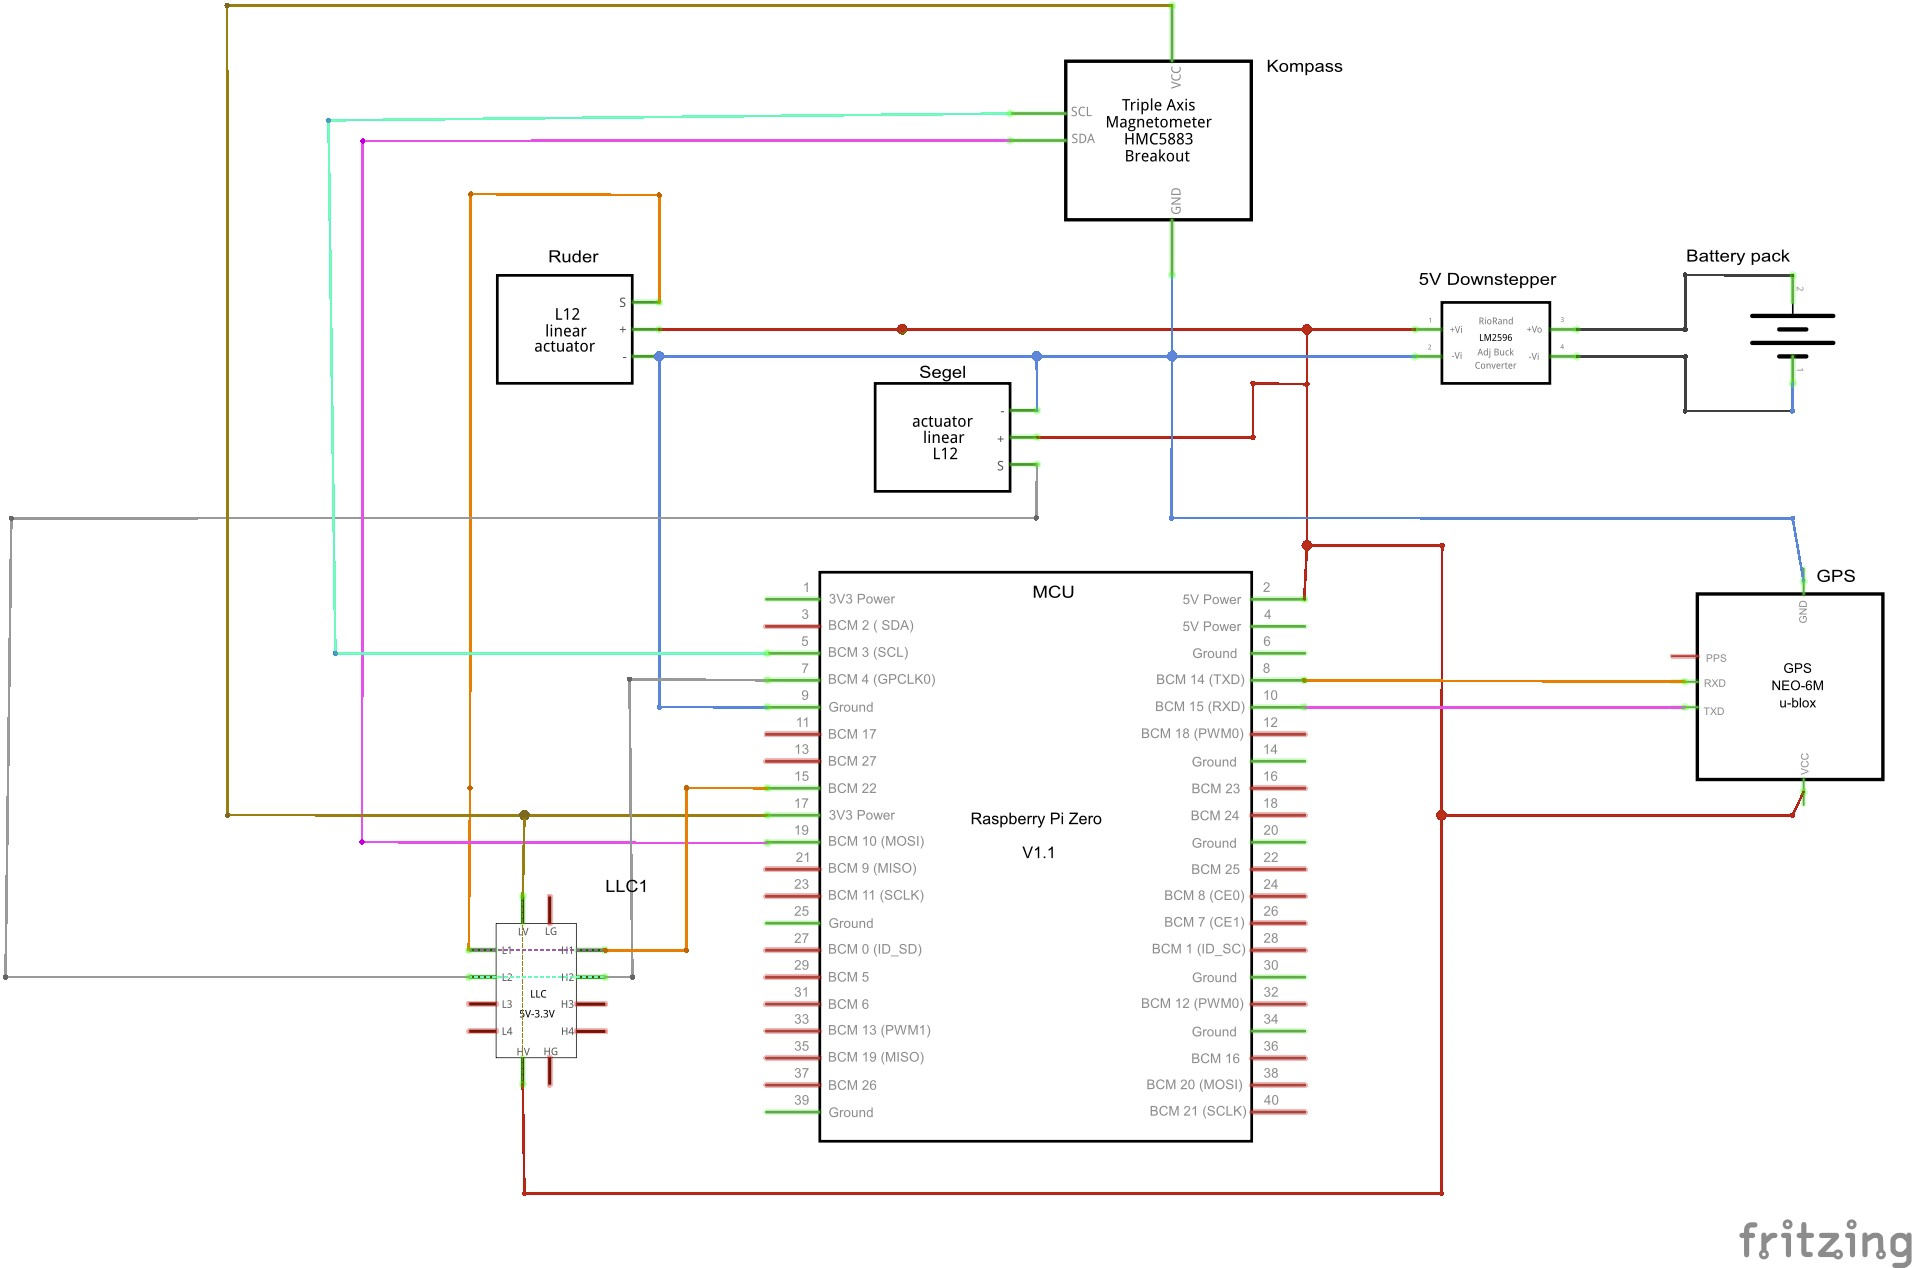
\includegraphics[angle=90,width=\textwidth,height=\textheight,keepaspectratio]{assets/schaltplan5.png}
    \caption{Schaltplan Bordelektronik}
\end{figure}

\includepdf[pages={2-4}]{assets/schematic.pdf}
\chapter{Algorithmus}
\label{appendix:algorythmus}







\begin{algorithm}
\caption{Berechne neuen Kurs}
\begin{algorithmic}[1]
\Function{BerechneNeuenKurs}{$\vec{v}_{\text{Boot}}, \vec{v}_{\text{Wind}}, \vec{v}_{\text{Ziel}}$}
    \State $\text{Skalarprodukt} \gets \vec{v}_{\text{Wind}} \cdot \vec{v}_{\text{Boot}}$
    
    \State $\vec{neuerKurs} \gets \vec{v}_{\text{Ziel}}$
    
    \If{$\text{Skalarprodukt} < -0.8$}
        \If{$\vec{v}_{\text{Wind}} \cdot \vec{v}_{\text{Ziel}} > -0.8$}
            \State $\vec{neuerKurs} \gets \vec{v}_{\text{Ziel}}$
            \State \Return \Call{Normalisiere}{$\vec{neuerKurs}$}
        \EndIf
        
        \State $n \gets 0$
        \While{$\vec{v}_{\text{Wind}} \cdot \vec{neuerKurs} < -0.8$ \textbf{und} $n < 1$}
            \State $n \gets n + 0.1$
            \State $\vec{neuerKurs1} \gets \vec{v}_{\text{Ziel}} + n \cdot \begin{bmatrix}0 & -1 \\ 1 & 0\end{bmatrix} \cdot \vec{v}_{\text{Ziel}}$
            \State $\vec{neuerKurs2} \gets \vec{v}_{\text{Ziel}} + n \cdot \begin{bmatrix}-1 & 0 \\ 0 & 1\end{bmatrix} \cdot \vec{v}_{\text{Ziel}}$
            
            \If{$\vec{neuerKurs1} \cdot \vec{v}_{\text{Ziel}} > \vec{neuerKurs2} \cdot \vec{v}_{\text{Ziel}}$}
                \State $\vec{neuerKurs} \gets \vec{neuerKurs1}$
            \Else
                \State $\vec{neuerKurs} \gets \vec{neuerKurs2}$
            \EndIf
        \EndWhile
        
        \State \Return \Call{Normalisiere}{$\vec{neuerKurs}$}
    \EndIf
\EndFunction
\end{algorithmic}
\end{algorithm}




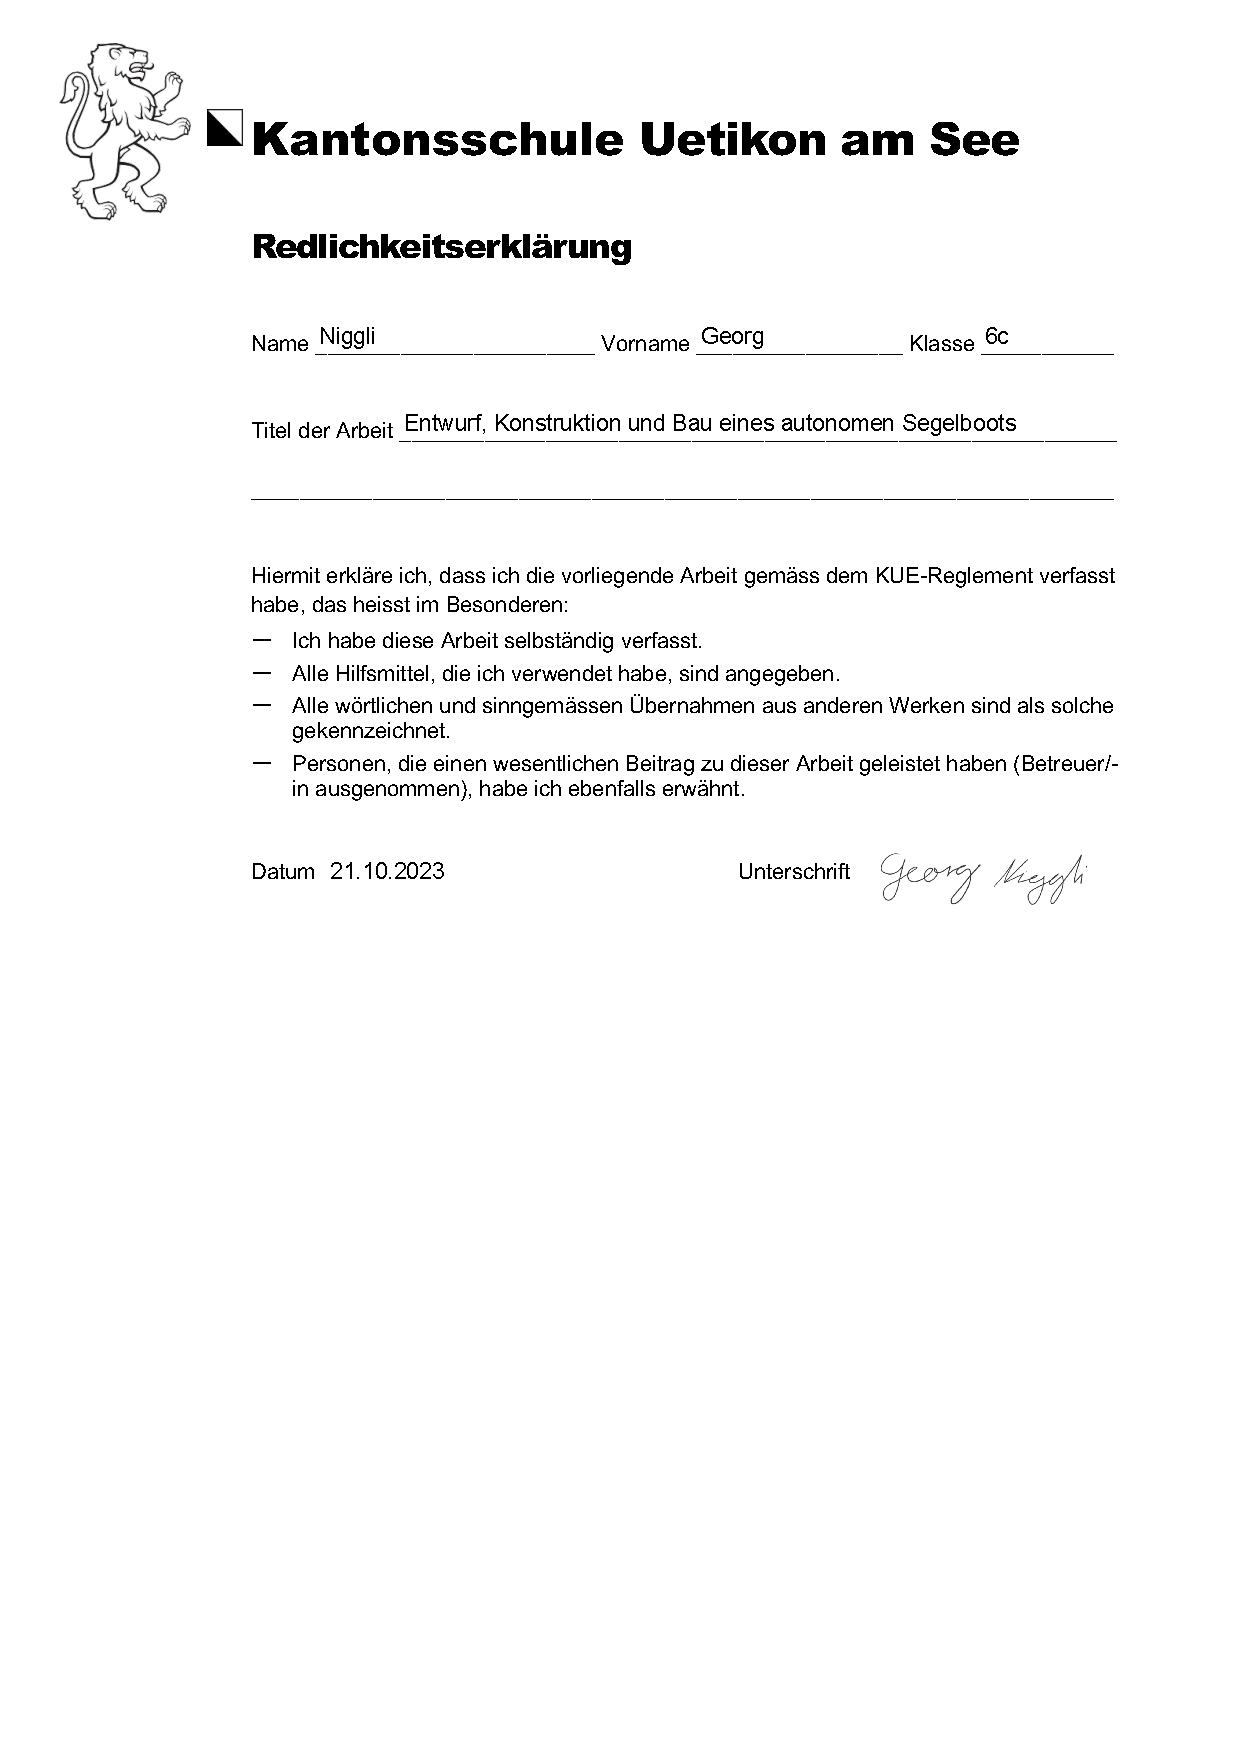
\includepdf[]{assets/redlichkeit.pdf}









\end{document}
